\documentclass[ 11pt
				,ngerman 
				,headsepline
				,headings=small
				,numbers=noenddot % Kein "." hinter der letzten Kapitelnummer --> 2.1 statt 2.1.
				,draft=false
				,BCOR=0mm % Wert für die Bindung 
				,DIV=12 % Wert für die größe des Textblocks
				,captions=tableheading
				,paper=a4
				,abstracton
				,twoside % Erlaubt beidseitigen Druck
                ]{scrreprt}
% Wählt den passenden Offset und Margin für das Deckblatt und wählt ein passenden Seitenlayout
\makeatletter
\newlength\offsetCoverPage
\newlength\marginCoverPage
\newcount\onesideprint
\if@twoside
\usepackage[a4paper, left=2.6cm, right=2.9cm, top=3.7cm, bottom=3.8cm]{geometry}
\offsetCoverPage=0.0cm
\marginCoverPage=0.25cm
\onesideprint=0
\else
\usepackage[a4paper, left=2.75cm, right=2.75cm, top=3.7cm, bottom=3.8cm]{geometry}
\offsetCoverPage=-0.10cm
\marginCoverPage=0cm
\onesideprint=1
\fi
\makeatother



%-----------------------------------------------------------------------------
% Größeninformationen:
% mit den gewählten Einstellungen beträgt die Textbreite (und damit auch die
% sinnvolle Bildbreite) ca. 158 mm
% Die Texthöhe beträgt etwa 215.0 mm, eine vollseitige Grafik sollte daher 
% maximal 200 mm hoch sein, halbseitige Grafiken entsprechend etwa 90 mm um
% genügend Raum für ein zweites Bild mit Bildunterschrift oder alternativ 
% Fließtext zu bieten
%-----------------------------------------------------------------------------

%-----------------------------------------------------------------------------
% Basispackete
%-----------------------------------------------------------------------------
\usepackage[utf8]{inputenc} 
%\usepackage[english]{babel} %Für einen englischen Text kommentiere die nächste Zeile und entferne den Kommentar dieser Zeile
\usepackage[ngerman]{babel} 
\usepackage{ifpdf} 
\usepackage{blindtext} % Um den lorem ipsum Text zu erzeugen
%\usepackage{svg}
\usepackage{epstopdf}
\usepackage[tableann,xcdraw]{xcolor}
%\usepackage{subfig} %für mehrere Bilder nebeneinander HACK#42


        
%-----------------------------------------------------------------------------
% Schrifteinstellungen
%-----------------------------------------------------------------------------
\usepackage{fourier} %PDF-compatible font "Utopia". There exists a free look-alike: Heuristica
\makeatletter % No warnings because of a replaced font
  \let\@font@info\@gobble
  \let\@font@warning\@gobble
\makeatother
\usepackage[official]{eurosym} % Eurosymbol
\DeclareUnicodeCharacter{20AC}{\euro} % The normale euro symbol via [Alt Gr][€] is replaced by a high quality one
\renewcommand{\caplabelfont}{\bfseries} % Fig. and Tab. are bold
\usepackage{color}
\definecolor{ercred}{RGB}{229,48,39}
\usepackage{setspace} % Change Linespread
\onehalfspacing % Linespread 1.5
\setlength\parskip{\medskipamount} % Small linespread between two paragraphs
\setlength\parindent{0pt} % No indentation in the first line of a new paragraph
\AtBeginDocument{
  \renewcommand{\labelitemi}{\(\triangleright\)} % re-definition of the bullet-points
  \renewcommand{\labelitemii}{\(\bullet\)}}

%\usepackage{watermark}
%\usepackage{color}
%\definecolor{light}{gray}{.50}

\usepackage{eso-pic}
%\usepackage{graphicx}
\usepackage{color}
\usepackage{type1cm}
\makeatletter
\AddToShipoutPicture{
	\setlength{\@tempdimb}{.5\paperwidth}
	\setlength{\@tempdimc}{.5\paperheight}
	\setlength{\unitlength}{1pt}
	\put(\strip@pt\@tempdimb,\strip@pt\@tempdimc){
		\makebox(0,0){
			\rotatebox{45}{
				\textcolor[gray]{0.9}{
					\fontsize{5cm}{5cm}
					\selectfont{
						Vertraulich
					}
				}
			}
		}
	}
}
\makeatother

%-----------------------------------------------------------------------------
% Seitenlayout
%-----------------------------------------------------------------------------

\usepackage[automark, autooneside=false]{scrlayer-scrpage}
% Für eine genauere Erklärung lies scrguide.pdf, ca. Seite 240
\automark[chapter]{chapter}
\automark*[section]{}
\interfootnotelinepenalty=10000 % Fußnoten nicht über zwei Seiten verteilen

%Kopfzeile einseitiger Druck
\ifnum\onesideprint=1
\pagestyle{scrheadings}
 \clearscrheadfoot
 \automark{chapter}
 \renewcommand\sectionmark[1]{\markright{\MakeMarkcase {\thesection\hskip .5em\relax#1}}} 
 \rohead{\ifnum\expandafter\pdfstrcmp\botmark=0 \rightmark\else\leftmark{} --- \rightmark\fi}
\ihead{\leftmark}
\ohead{\rightmark}
\cfoot{\pagemark}
\fi
%-----------------------------------------------------------------------------
% Tabellen
%-----------------------------------------------------------------------------
\usepackage{longtable}
\usepackage{multirow}
\usepackage{booktabs} % Erstelle besser aussehende Tabellen, nutze \toprule, \midrule, \bottomrule für horizontale Linien
\usepackage[point]{rccol} % Werte werden über das Kommata ausgerichtet
\usepackage{tabularx}
\newcolumntype{L}[1]{>{\raggedright\arraybackslash}p{#1}}
\newcolumntype{C}[1]{>{\centering\arraybackslash}p{#1}}
\newcolumntype{R}[1]{>{\raggedleft\arraybackslash}p{#1}}
%-----------------------------------------------------------------------------
% Abbildungen
%-----------------------------------------------------------------------------
\usepackage{subfigure}
\usepackage{float}
% Reduzierung der Anzahl von "Float-Only"-Seiten
\renewcommand{\topfraction}{0.85}
\renewcommand{\textfraction}{0.1}
\renewcommand{\floatpagefraction}{0.75}

%-----------------------------------------------------------------------------
% Mathematik
%-----------------------------------------------------------------------------
\usepackage{amsmath}
\usepackage{amssymb}
\usepackage{array}
\usepackage[cdot,thickqspace,squaren,textstyle]{SIunits} % SI-Einheiten können mit Namen eingegeben werden

 
%-----------------------------------------------------------------------------
% Verweise und Zitate
%-----------------------------------------------------------------------------
\usepackage{varioref}
\usepackage{natbib}    %[square]{natbib}
\usepackage{bibunits}

%-----------------------------------------------------------------------------
% PDF-Setup
%-----------------------------------------------------------------------------
\ifpdf
	%wir benutzen PDFLaTeX
	\usepackage[pdftex]{graphicx} 
	\pdfimageresolution=100
	\pdfminorversion=7
	\pdfcompresslevel=9
	\usepackage[pdftex,
		urlcolor=blue,
		linktoc=all,
		colorlinks=true,
		linkcolor=black,
		citecolor=black,
		pdfview=FitH,
		pdfstartview=FitH,
		plainpages=false]{hyperref}
	\hypersetup{
		pdfauthor={Your Name here},
        pdftitle={Name of your thesis},
        pdfsubject={},
        pdfkeywords={several helpful keywords},
        pdfproducer={LaTeX with hyperref},
        pdfcreator={pdflatex}}
    \usepackage[figure,figure*]{hypcap}
\else
	%DVI oder PS Ausgabe
	\usepackage{graphicx} 

\fi


%-----------------------------------------------------------------------------
% JETZT GEHTS LOS!
%-----------------------------------------------------------------------------
\begin{document}
\pagestyle{empty}
\newcounter{Hilfszaehler}

%-----------------------------------------------------------------------------
% Deckblatt
%-----------------------------------------------------------------------------
\begin{titlepage}
\begin{addmargin}{\offsetCoverPage} 
%TODO Um das RWTH-Logo zu benutzen, musst du das Formblatt RWTH-Logo Deutsch aus der Datei Formulare.txt
%TODO ausfüllen und es dem ZPA schicken!

%-----------------------------------------------------------------------------
% Platzierung der Kopfzeile(Nummer und Logo)
%-----------------------------------------------------------------------------
\setlength{\unitlength}{1cm}
\begin{picture}(0,0)
\put(5,0.68){
\includegraphics[width =0.15\textwidth]{Pictures/Emerson-Logo}}
\put(7.977,0.68){
\includegraphics[width = 0.5\textwidth]{Pictures/rwth_eerc_rgb_ohne_Schutzraum}}
%TODO Ändere die Nummer deiner Arbeit, und wenn noetig die Bezeichnung(BA, MA, PA)
%TODO Die Abkürzungen sind Deutsch, auch wenn die Arbeit in Englisch verfasst wird
\put(0,1.32){\fontfamily{phv}\selectfont\huge{BA 000}}
\end{picture}
\end{addmargin}
%-----------------------------------------------------------------------------
% Titel deiner Arbeit
%-----------------------------------------------------------------------------
\addvspace{2.6cm}
%TODO Formaenderung des Titels
\begin{addmargin}[\marginCoverPage]{0cm}
\begin{center}
{\fontfamily{phv}\selectfont\huge Bachelorarbeit} 
\end{center}

{\Large \par}
\addvspace{1.5cm}
\begin{center}
%TODO Wenn du ein "Sperrvermerk" für deine Arbeit brauchst, entferne den Kommentar in der naechsten Zeile
\textbf{{\color{ercred}\fontfamily{phv}\selectfont{\huge Sperrvermerk}}}\\

%TODO  Der Englische Titel deiner Arbeit wird nach dem "\huge" in der naechsten Zeile geaendert
\textbf{\fontfamily{phv}\selectfont{\huge Modellgestützte Untersuchung und experimentelle Validierung von Verdampferverschaltungen zur thermischen Leistungssteigerung für den Einsatz in Kühlmöbeln}}
\end{center}

\addvspace{1.5cm}
\begin{center}
%TODO Falls der deutsche Name noch noetig ist, kommt er in die naechste Zeile
{\fontfamily{phv}\selectfont Model-based investigation and experimental validation of evaporator interconnections for thermal performance enhancement for use in refrigerated display cabinets}
\end{center}

%-----------------------------------------------------------------------------
% Namen, Daten
%-----------------------------------------------------------------------------
\vfill
\begin{center}
\begingroup
\fontfamily{phv}\selectfont
%TODO Bitte aendere das Datum deiner Abgabe
Aachen, April 2018 \\
\addvspace{0.5cm}
%TODO Bitte aendere deinen Namen und Matrikelnummer in den naechsten beiden Zeilen
\textbf{Tim Klebig} \\
Matrikelnummer: 335421 \\
\addvspace{0.5cm}
%TODO Deine Betreuer. Achte auf die richtige Schreibweise des Titels.
Betreuer:\\
Christian Vering, M. Sc. \\
Dr.-Ing. Andreas Bühring \\
Univ.-Prof. Dr.-Ing. Dirk Müller \\
\addvspace{0.5cm}
%TODO  Eingabe der richtigen Anschrift des Instituts.
Diese Arbeit wurde vorgelegt am:\\
E.ON Energy Research Center | ERC \\
Institute for Energy Efficient Buildings and Indoor Climate | EBC\\
(Lehrstuhl für Gebäude- und Raumklimatechnik)\\
Mathieustraße 10, 52074 Aachen\\
\endgroup
\end{center}
\end{addmargin}
\end{titlepage}



%-----------------------------------------------------------------------------
% Setup von speziellen Seiten(Abbildungsverzeichnis, Nomenklatur etc.
%-----------------------------------------------------------------------------
\cleardoublepage
\pagenumbering{Roman} % Romanische Nummerierung
%-----------------------------------------------------------------------------
% Englische und Deutsche Kurzfassung. Beide notwendig
%-----------------------------------------------------------------------------
\clearpage
\refstepcounter{Hilfszaehler}
\renewcommand\abstractname{Kurzfassung}
\begin{abstract}
Überall dieselbe alte Leier. Das Layout ist fertig, der Text lässt auf sich warten. Damit das Layout nun nicht nackt im Raume steht und sich klein und leer vorkommt, springe ich ein: der Blindtext. Genau zu diesem Zwecke erschaffen, immer im Schatten meines großen Bruders »Lorem Ipsum«, freue ich mich jedes Mal, wenn Sie ein paar Zeilen lesen. Denn esse est percipi - Sein ist wahrgenommen werden.

Und weil Sie nun schon die Güte haben, mich ein paar weitere Sätze lang zu begleiten, möchte ich diese Gelegenheit nutzen, Ihnen nicht nur als Lückenfüller zu dienen, sondern auf etwas hinzuweisen, das es ebenso verdient wahrgenommen zu werden: Webstandards nämlich. Sehen Sie, Webstandards sind das Regelwerk, auf dem Webseiten aufbauen. So gibt es Regeln für HTML, CSS, JavaScript oder auch XML; Worte, die Sie vielleicht schon einmal von Ihrem Entwickler gehört haben. Diese Standards sorgen dafür, dass alle Beteiligten aus einer Webseite den größten Nutzen ziehen.

Im Gegensatz zu früheren Webseiten müssen wir zum Beispiel nicht mehr zwei verschiedene Webseiten für den Internet Explorer und einen anderen Browser programmieren. Es reicht eine Seite, die - richtig angelegt - sowohl auf verschiedenen Browsern im Netz funktioniert, aber ebenso gut für den Ausdruck oder die Darstellung auf einem Handy geeignet ist. Wohlgemerkt: Eine Seite für alle Formate. Was für eine Erleichterung. Standards sparen Zeit bei den Entwicklungskosten und sorgen dafür, dass sich Webseiten später leichter pflegen lassen. Natürlich nur dann, wenn sich alle an diese Standards halten. Das gilt für Browser wie Firefox, Opera, Safari und den Internet Explorer ebenso wie für die Darstellung in Handys. Und was können Sie für Standards tun? Fordern Sie von Ihren Designern und Programmieren einfach standardkonforme Webseiten. Ihr Budget wird es Ihnen auf Dauer danken. Ebenso möchte ich Ihnen dafür danken, dass Sie mich bin zum Ende gelesen

This abstract has 300 words

\end{abstract}
\renewcommand{\abstractname}{Abstract}
\begin{abstract}

 
\end{abstract}

\cleardoublepage

%-----------------------------------------------------------------------------
% Inhaltsverzeichnis
%-----------------------------------------------------------------------------
\pagestyle{plain.scrheadings}
\setcounter{secnumdepth}{2}
\setcounter{tocdepth}{2}
\tableofcontents



%-----------------------------------------------------------------------------
% Abbildungsverzeichnis
%-----------------------------------------------------------------------------
\clearpage
\refstepcounter{Hilfszaehler}
\addcontentsline{toc}{chapter}{Abbildungsverzeichnis}
\listoffigures

%-----------------------------------------------------------------------------
% Tabellenverzeichnis
%-----------------------------------------------------------------------------
\clearpage
\refstepcounter{Hilfszaehler}
\addcontentsline{toc}{chapter}{Tabellenverzeichnis}
\listoftables


%-----------------------------------------------------------------------------
% Nomenklatur
%-----------------------------------------------------------------------------
\clearpage
\refstepcounter{Hilfszaehler}
\addcontentsline{toc}{chapter}{Nomenklatur}
\chapter*{Nomenklatur}
\begin{onehalfspacing}
\begin{longtable}[h]{p{0.15\textwidth} p{0.65\textwidth} p{0.1\textwidth}}
		\caption*{\textbf{Formelzeichen und Einheiten}} \\
		\\
		\textbf{Symbol} & \textbf{Bedeutung} & \textbf{Einheit} \\ %\hline 
		\endhead
		\\
		\multicolumn{3}{c}{Fortsetzung auf der nächsten Seite} \\
		\endfoot
		\multicolumn{3}{c}{ } \\
		\endlastfoot
		
		$A$ & Fläche & \squaremetre\\
		$a$&Koeffizient&---\\
		$c$ & Schallgeschwindigkeit & \metre\per\second\\
		$c_{p}$&spezifische Wärmekapazität bei konstantem Druck&\joule\per(\kilogram\usk\kelvin)\\
		$C$&Wärmekapazität&\watt\per\kilogram\\		
		$\dot{C}$&Wärmekapazitätsstrom&\watt\per(\kilogram\usk\second)\\
		$C$&Koeffizient&---\\
		$d$ & Durchmesser & \metre\\
		$E$ & Verteilfaktor & ---\\
		$EER$ & Energy Efficiency Ratio & ---\\
		$Fr$&Froudezahl& ---\\
		$h $ & Enthalpie & \joule\\	
		$K$&Hilfsgröße&---\\
		$l$ & Länge & \metre\\
		$\dot{M}$ & Massenstrom & \kilogram\per\second\\	
		$\dot{m}$ & spezifischer Massenstrom & \kilogram\per(\second\usk\metre)\\
		$NTU$ &Anzahl der Übertragungseinheiten (\emph{engl.: Number of transfer units}) & ---\\
		$P$ & Leistung & \watt\\		
		$p$ & Druck & \pascal\\
		$p$ & Druck & \bbar\\
		$\dot{Q}$ & Wärmestrom & \watt\\
		$Re$ & Reynoldszahl & ---\\
		$T$ & Temperatur & \kelvin\\
		$t$ & Zeit & \second\\
		$k$ & Wärmedurchgangskoeffizient & \watt\per(\squaremetre\usk\kelvin)\\		
		$V$ & Volumen & \cubic\meter\\
		$W$ & Wärmeleitwiderstand & \kelvin\per\watt\\
		$\dot{V}$&Volumenstrom&\cubic\meter\per\second\\
		$x$ & Dampfanteil & \%\\
		$Y$ & Wasserbeladung der Luft & \gram\per\kilogram\\
		
		
\end{longtable}

\begin{longtable}[h]{p{0.15\textwidth} p{0.65\textwidth} p{0.1\textwidth}}
		\caption*{\textbf{Griechische Formelzeichen}} \\
		\\
		\textbf{Symbol} & \textbf{Bedeutung} & \textbf{Einheit} \\ %\hline 
		\endhead
		\\
		\multicolumn{3}{c}{Fortsetzung auf der nächsten Seite} \\
		\endfoot
		\multicolumn{3}{c}{ } \\
		\endlastfoot


		$\alpha$ & Wärmeübergangskoeffizient & \watt\per(\squaremetre\usk\kelvin)\\
		$\beta$ & Volumenstromverhältnis von flüssiger und gasförmiger Phase & \pascal\\
		$\gamma$ & Versperrungsfaktor & \pascal\\
		$\epsilon$ & Hilfsgröße & \watt\\
		$\epsilon$ & Effektivität & ---\\
		$\eta$ & dynamische Viskosität & \kilogram\per(\metre\usk\second)\\
		$\lambda$ & Wärmeleitwert & \watt\per(\metre\usk\kelvin)\\
		$\nu$&kinematische Viskosität&cSt\\
		$\omega$&Löslichkeit& (\gram KM)\per(\gram Öl)\\
		$\Phi$ & thermische Leistung & \watt\\
		$\psi$ & Hilfsgröße & ---\\
		$\varrho$& Massendichte&\kilogrampercubicmetre\\
			$\sigma$&Temperaturspreizung&\kelvin\\
		$\vartheta $ & Temperatur  & \degreecelsius\\
		$\Delta\vartheta $ & Temperaturdifferenz  &\kelvin\\
		$\xi$ & Reibungsbeiwert & ---\\
		
\end{longtable}
\clearpage

\begin{longtable}[h]{p{0.15\textwidth} p{0.75\textwidth}}
		\caption*{\textbf{Indizes und Abkürzungen}} \\
		\\
		\textbf{Symbol} & \textbf{Bedeutung} \\ %\hline 
		\endhead
		\\
		\multicolumn{2}{c}{Fortsetzung auf der nächsten Seite} \\
		\endfoot
		\multicolumn{2}{c}{ } \\
		\endlastfoot
		
		A & Fluid A \\
		B & Fluid B \\
		Al & Aluminium\\ 
		aus & Ausgang\\		
		Cu & Kupfer \\
		cd & Verflüssiger (\emph{engl.: condensor})\\
		cp & Verdichter (\emph{engl.: compressor})\\ 
		E & ebene Strömung \\   
		EES & Engineering Equation Solver \\
		ein & Eingang \\
		el & elektrisch \\
		ev & Verdampfer (\emph{engl.: evaporator})\\
		F & Flüssigkeit\\	
		G & Gas \\
		i & innen \\
		K & (Kälte-)Kreis\\
		KM & Kältemittel\\
		NI-LabView & Programmiersprache und Entwicklungsumgebung für die Messdatenerfassung der Firma National Instruments\\
		L & Luft\\
		max & Maximum \\
		min & Minimum \\
		P & Durchgang (\emph{engl.: Pass})\\
		r & Verhältnis (\emph{engl.: ratio})\\
		sat & Sättigungszustand (\emph{engl.: saturated})\\
		SH & Überhitzung (\emph{engl.: Superheat})\\
		W & Wasser \\
		WÜ & Wärmeübertrager \\
		
\end{longtable}
\end{onehalfspacing}


%-----------------------------------------------------------------------------
% Vorwort, kommentiere die Zeile wenn nicht nötig
%-----------------------------------------------------------------------------
%\clearpage
%\refstepcounter{Hilfszaehler}
%\addcontentsline{toc}{chapter}{Vorwort}
%%\newpage\thispagestyle{empty}~
\chapter*{Vorwort}

patata Lorem ipsum dolor sit amet, consectetuer adipiscing elit, sed diam nonummy nibh euismod tincidunt ut laoreet dolore magna aliquam erat volutpat. Ut wisi enim ad minim veniam, quis nostrud exerci tation ullamcorper suscipit lobortis nisl ut aliquip ex ea commodo consequat. Duis autem vel eum iriure dolor in hendrerit in vulputate velit esse molestie consequat, vel illum dolore eu feugiat nulla facilisis at vero et accumsan et iusto odio dignissim qui blandit praesent luptatum zzril delenit augue duis dolore te feugait nulla facilisi (Tabelle\,\ref{tab:Table}). Lorem ipsum dolor sit amet, consectetuer adipiscing elit, sed diam nonummy nibh euismod tincidunt ut laoreet dolore magna aliquam erat volutpat.Ut wisi enim ad minim veniam, quis nostrud exerci tation ullamcorper suscipit lobortis nisl ut aliquip ex ea commodo consequat. Duis autem vel eum iriure dolor in hendrerit in vulputate velit esse molestie consequat, vel illum dolore eu feugiat nulla facilisis at vero et accumsan et iusto odio dignissim qui blandit praesent luptatum zzril delenit augue duis dolore te feugait nulla facilisi. Nam liber tempor cum soluta nobis eleifend option congue nihil imperdiet doming id quod mazim placerat facer possim assum. Ut wisi enim ad minim veniam, quis nostrud exerci tation ullamcorper suscipit lobortis nisl ut aliquip ex ea commodo consequat. Duis autem vel eum iriure dolor in hendrerit in vulputate velit esse molestie consequat, vel illum dolore eu feugiat nulla facilisis at vero et accumsan et iusto odio dignissim qui blandit praesent luptatum zzril delenit augue duis dolore te feugait nulla facilisi. Nam liber tempor cum soluta nobis eleifend option congue nihil imperdiet doming id quod mazim placerat facer possim assum.


%-----------------------------------------------------------------------------
% Setup Normale Seiten(Neue Nummerierung)
%-----------------------------------------------------------------------------
\cleardoublepage
\clearpage
\pagenumbering{arabic}
\pagestyle{scrheadings}%\ihead{\leftmark}\chead{}\ohead{\rightmark}
\automark[chapter]{chapter}
\automark*[section]{}

%-----------------------------------------------------------------------------
% Füge hier deine Kapitel hinzu
%-----------------------------------------------------------------------------
%\watermark{\fontsize{30pt}{70pt}\selectfont\textcolor{light}{Vertraulich}}

\chapter{Motivation}
\label{cha:Motivation}

Im Fokus der Arbeit steht ein vertikales Supermarktkühlmöbel für Normalkühlung, welches mit Propan (R290) betrieben wird \cite{DINDeutschesInstitutfurNormunge.V..b}. Propan findet vor dem Hintergrund der F-Gas-Verordnung und aufgrund der hohen volumetrischen Kälteleistung immer häufiger in Kälteanlagen Verwendung \cite{EUParlamentRat.2006},\cite{Huber.2016},\cite{Moons.2013}. Sicherheitsnormen beschränken die maximale Füllmenge eines Kältekreises mit Propan auf \unit{150}{\gram} \cite{DINDeutschesInstitutfurNormunge.V..2014b}. Das AHT-Kühlmöbel, für dessen Produktion die Firma Emerson Scrollverdichter liefert, ist nicht in der Lage die Zieltemperatur, die zwischen \unit{-1}{\celsius} und \unit{5}{\celsius} liegt, über die gesamte Warenausstellfläche gleichmäßig zu erreichen. Es werden Untersuchungen in einer Klimakammer durchgeführt, um Gründe für die unzureichende Produktkühlung zu finden und um die Kälteleistung der Kältekreise zu erhöhen. Das Ziel dieser Untersuchungen ist die Identifikation eines optimalen Betriebspunkts durch Zusammenstellung geeigneter Komponenten und Maßnahmen. Diese werden im Rahmen der Untersuchungen hinsichtlich der erzielten Kälteleistung und der Anlageneffizienz bewertet. 
Vorausgehende Arbeiten umfassen die Installation von Temperatur- und Drucksensoren am Kältekreis und an den Produktdummys, um das Verhalten des Systems zu erfassen und analysieren zu können sowie den Einbau kleinerer Plattenwärmeübertrager als Kondensatoren. Letzteres zielt auf eine Reduzierung des internen Volumens der Kältekreise, um den Mangel an Kältemittel zu kompensieren. Zudem wurden zur genaueren Regelung der Überhitzung thermische durch elektronische Expansionsventile ersetzt. Eine weitere durchgeführte Veränderung ist der Wechsel eines Glykol-Wasser-Gemischs zu Wasser als Wärmetransportmedium für die Kondensation.
Dabei werden folgende experimentelle Untersuchungen durchgeführt:

\begin{itemize} 
\item Betrieb mit dem Verdichter ZB09KAU-TFD als Standard- und als Hybridausführung
\item Betrieb mit den Esterölen 3MAF und HATCOL~4467
\item Anpassung der Länge der Abtauintervalle
\item Änderung der Verschaltung der Verdampferpässe
\end{itemize}

Mithilfe einer geeigneten Software wird ein Simulationsmodell entwickelt, um die Leistung des Verdampfers in einer anderen Verschaltung versuchsunabhängig vorauszusagen. Anschließend wird dieses anhand der durchgeführten Untersuchungen validiert. 


\chapter{Stand der Forschung}
\label{cha:Technik}

Dieses Kapitel bietet eine Übersicht über den Prüfstand, die Messdatenerfassung und das Simulationsmodell. Es werden, die für das Verständnis notwendigen Grundlagen von Kältekompressionsmaschinen sowie die Berechungsgleichungen des Modells erläutert.

\section{Kompressionskältemaschinen}
\label{sec:Stand der Technik}

Kältekompressionsmaschinen

\subsection{Komponenten einer Kältekompressionsmaschine}
\label{subsec:Komponenten einer Kältekompressionsmaschine}

\subsubsection{Verdichter}
\label{subsubsec:Verdichter}

Mithilfe des Verdichters wird gasförmiges Kältemittel auf ein hohes Druck- und Temperaturniveau verdichtet. Im Anwendungsgebiet der Normalkühlung werden vor allem Hubkolben- und Scrollverdichter eingesetzt. Scrollkompressoren zeichnen sich durch hohe Effizienz aus. Diese verfügen über eine sich auf einer kreisförmigen Bahn bewegenden Spirale. Diese Bahn wird durch eine stationäre Spirale vorgegeben. Durch das bei Rotation zur Spiralmitte kleiner werdende Volumen findet die Verdichtung statt. Scrollkompressoren dissipieren wegen der aneinander reibenden Spiralen viel Hitze und können sehr heiß werden. Damit der Verdichter keinen Schaden nimmt muss eine ausreichende Ölschmierung jederzeit gewährleistet sein. 


\subsubsection{Kondensator}
\label{subsubsec:Kondensator}

Im Kondensator wird gasförmiges, überhitztes Kältemittel durch Wärmeabgabe an ein anderes Fluid enthitzt, kondensiert und idealerweise unterkühlt. Neben den klassischen Luft-Kältemittel-Wärmeübertragern finden oft Wasser-Kältemittel-Wärmeübertrager Anwendung. Diese werden als Plattenwärmeübertrager ausgeführt und ermöglichen aufgrund der höheren Wärmekapazität von Wasser bzw. Sole gegenüber Luft kleineren Bauraum bei gleicher Leistung. Der Verflüssigungsdruck ergibt sich aus der Wassereintritts- und –austrittstemperatur, der wärmeübertragenden Fläche sowie der Massenstöme von Wasser und Kältemittel \cite{Kulterer.2007}.

\subsubsection{Expansionsventil}
\label{subsubsec:Expansionsventil}


Im Expansionsventil wird der Druck des Kältemittels nach dem Kondensator auf ein niedriges Druckniveau gedrosselt. Dies hat ein Absinken der Sättigungstemperatur zur Folge. Die Enthalpie des Kältemittels bleibt dabei konstant. Durch die bei sinkendem Druck größer werdende Verdampfungsenthalpie hat das Kältemittel nach der Drosselung einen größeren Dampfanteil als vor dem Ventil. Zum Schutz des Expansionsventiles vor Beschädigung durch Gasblasen und um ein fehlerfreies Regelverhalten zu garantieren ist es nötig das Kältemittel vor dem Ventil vollständig zu kondensieren und zu unterkühlen. Gleichzeitig hat das Expansionsventil die Aufgabe die Überhitzung des Kältemittels auf einen vorgegebenen Wert zu regeln und konstant zu halten. Die Überhitzung ist die Differenz zwischen der Sättigungstemperatur des Kältemittels und dessen tatsächlicher Temperatur. Die Temperatur am Austritt des Verdampfers wird durch einen Temperatursensor an der Saugleitung erfasst. Um das Regelverhalten zu verbessern haben diverse Ventile einen zusätzlichen Drucksensor in der Saugleitung. Dadurch wird eine Verfälschung der Überhitzungsregelung durch Druckabfall über den Verdampfer eliminiert. Elektronische Expansionsventile ermöglichen gegenüber thermostatischen Ventilen ein sehr präzises und schnelles Regelverhalten. 

\subsubsection{Verdampfer}
\label{subsubsec:Verdampfer}

Im Verdampfer nimmt das Kältemittel bei niedrigem Druck und entsprechend niedriger Sättigungstemperatur die Wärme des zu kühlenden Fluids auf und verdampft dabei. Die Verdampfungstemperatur soll dabei etwa \unit{10}{\kelvin} unter der Zielprodukttemperatur liegen. In steckerfertigen Kühlmöbeln finden ausschließlich Luft-Kältemittel-Wärmeübertrager Anwendung. Um die wärmeübertragende Fläche zu vergrößern sind die Verdampferrohre mit Lamellen aus Aluminium bestückt. Diese haben für den Einsatzbereich der Normalkühlung Abstände von \unit{4}{\milli\metre} bis \unit{5}{\milli\metre}. Damit verhindert wird, dass flüssiges Kältemittel den Verdichter schädigt, wird das Kältemittel um etwa \unit{8}{\kelvin} überhitzt.


\subsection{Propan in Kälteanlagen}
\label{subsec:Propan in Kälteanlagen}

Der Kohlenwasserstoff Propan (R290) bietet eine umweltfreundliche Alternative zu Kältemitteln wie R22 oder R407c. Propan ist ein natürliches Kältemittel und besitzt eine sehr hohe Verdampfungsenthalpie. Bei gleicher Kälteleistung sind viel geringere Massenströme nötig. Dies resultiert in einem geringeren Energieverbrauch und damit einer höheren Anlageneffizienz.
Es ist mit einem GWP von 0 weder ozonschädlich noch gesundheitsschädlich. Die Verwendung von Propan benötigt aber wegen hoher Entflammbarkeit ein umfassendes Sicherheitkonzept für den Fall von Leckagen \cite{BitzerKuhlmaschinenGmbH.2014},\cite{Huber.2011}.
Um steckerfertige Kühlmöbel ohne spezielle Sicherheitsvorkehrungen betreiben zu können ist die maximale Füllmenge auf \unit{150}{\gram} pro Kältekreis beschränkt.





\subsection{Kältemittelöle}
\label{subsec:Kältemittelöle}

Öl in Kälteanlagen hat mehrere Aufgaben. Zur Sicherstellung der Funktionalität des Verdichters ist eine Ölmindestfüllmenge erforderlich. Die Hauptaufgabe des Öles ist eine ausreichende Schmierung des Verdichters, damit der Verschleiß der sich bewegenden Komponenten auf ein Minimum reduziert wird.  Während des Betriebs dissipiert aufgrund von Reibung Wärme, welche an Kältemittel, Öl und über das Gehäuse an die Umgebung abgegeben wird. \newline
Die zweite Aufgabe des Öles ist die Motorkühlung. Das Öl wird damit nur im Verdichter einer Kälteanlage benötigt. Es ist bedingt durch die Bauform des Verdichters nicht möglich den Mittransport eines Teils des Öles in den Kältekreis zu verhindern. Öl erfüllt nur im Verdichter den Zweck seiner Verwendung. In den Wärmeübertragern herrschen andere Drücke und Temperaturen als im Verdichter, was sich auf die physikalischen Eigenschaften des Öles auswirkt. Dort ist die Löslichkeit des Kältemittels im Öl höher, d.h. das Öl ist in der Lage mehr Kältemittel aufzunehmen und dadurch die nutzbare Kältemittelfüllmenge zu reduzieren. \newline
In Kälteanlagen eingesetzte Öle sind Mineralöle und Esteröle. Die im Rahmen der Arbeit untersuchten Öle HATCOL~4467 und 3MAF sind Esteröle, d.h. sie wurden eigens für die Anwendung in einer Kälteanlage synthetisiert \cite{ChemturaCorporation.2017},\cite{LubrizolCorporation.2015}. 
Die in diesem Abschnitt vorgestellten Gleichungen erlauben, unter Berücksichtigung der  Temperaturen und Drücke in den untersuchten Komponenten des Kältekreises, eine Berechnung der Öldichte, der kinematischen Viskosität und der Löslichkeit des Kältemittels im jeweiligen Öl \cite{EmersonClimateTechnologies.b}. Die Berechnungen dienen dem Vergleich beider Öle hinsichtlich der Erhöhung der Kälteleistung. In den folgenden Gleichungen bezeichnet $T$ die Temperatur des Öles in $\kelvin$ und $p$ den Druck in der jeweiligen Komponente in $\bbar$. Die Koeffizienten $a_1$ bis $a_9$ sind je nach Öl und Gleichung verschieden.

Die Öldichte $\rho$ in $\frac{\kilo\gram}{\cubic\metre}$ ergibt sich gemäß Gleichung~\ref{eq:1}: 

\begin{equation}
\label{eq:1}
\rho = a_{1} + a_{2}T + a_{3}T^2 + \omega(a_{4}+ a_{5}T + a_{6}T^2) + \omega^2(a_{7}+ a_{8}T + a_{9}T^2)
\end{equation}

Die Berechnung der kinematische Viskosität $\nu$ in $cSt$ erfolgt gemäß Gleichung~\ref{eq:3}:

\begin{align}
\label{eq:3}
	\begin{split}
		\ln(\ln(\nu + 0.7 + e^{-\nu} K_{0} (\nu + 1.244068))) =~ 
		&a_{1} + a_{2}\ln{T} + 	a_{3}\ln^2{T} \\
		&+ \omega(a_{4} + a_{5}\ln{T} + a_{6}\ln^2{T}) \\
		&+ \omega^2(a_{7} + a_{8}\ln{T} + a_{9}\ln^2{T}) 
	\end{split}
\end{align}

mit der Hilfsgröße $K_0$ gemäß Gleichung~\ref{eq:3_1}:

\begin{equation}
\label{eq:3_1}
K_0 = BesselK(\nu + 1.244068 , 0)
\end{equation}

Gleichung~\ref{eq:2} ermöglicht eine Berechnung der Löslichkeit $\omega$ des Kältemittels in $\frac{\gram KM}{\gram Öl}$. 

\begin{equation}
\label{eq:2}
\log(p) = a_{1} + \frac{a_{2}}{T} + \frac{a_{3}}{T^2} + \log(\omega)( a_{4} + \frac{a_{5}}{T} + \frac{a_{6}}{T^2}) + \log^2(\omega)( a_{7} + \frac{a_{8}}{T} + \frac{a_{9}}{T^2})
\end{equation}

Eine iterative Berechnung liefert eine Lösung für das Gleichungssystem.

\subsection{Abtauung}
\label{subsec:Abtauung}

Die Abtauregelung eines Kühlmöbels erfüllt den Zweck, dessen Verdampfer in regelmäßigen Abständen zu enteisen. Es wird zwischen elektrischer Abtauung, Heißgasabtauung und Umluftabtauung unterschieden. Bei einer elektrischen Abtauung wird das Eis mithilfe von Heizwiderständen im Verdampferpaket abgetaut. Eine Heißgasabtauung erfolgt mittels einer Systemumkehr des Kältekreises. Hierbei wird überhitztes Kältemittel in den Verdampfer geleitet und taut das Eis effektiv vom Entstehungspunkt ab. Die Umluftabtauung bezeichnet die einfachste Abtauregelung. Hierbei werden die Verdichter ausgeschaltet während die Verdampferlüfter weiterlaufen. Durch die wärmer werdende Luft wird das Eis langsam entfernt. Mittels einer Kondensatpumpe wird das aufgetaute Eis aus dem Kühlmöbel entfernt. \newline
Der Abtauung wird entweder in einem vorgegebenen Zeitintervall oder mittels einer Bedarfsdetektion eingeleitet. Bei einer bedarfsgerechten Abtauung wird die Temperaturdifferenz der Luft über den Verdampfer erfasst. Sinkt diese innerhalb des vorgegebenen Abtauintervalls unter einen bestimmten Wert, wird die Abtauung zu diesem Zeitpunkt eingeleitet.


\section{Das Kühlregal}
\label{sec:Das Kühlregal}

Der Mittelpunkt der durchgeführten Untersuchungen ist ein vertikales Verkaufskühlmöbel der Firma AHT.
Es umfasst auf einer Länge von \unit{3,75}{\metre} vier Regalböden um Produkte zu kühlen und auszustellen. Ein von oben herabfallender Luftschleier ermöglicht ein türloses Design des Regals. Ein Nachtbetrieb mit geschlossener Jalousie ist möglich. Abbildung~\ref{fig:IDC150} zeigt die Kältekreise des Kühlmöbels und die Positionen der Sensoren \cite{DINDeutschesInstitutfurNormunge.V..1998}. Die Kälteerzeugung wird durch drei seperate Kältekreisläufe gewährleistet. Das verwendete Kältemittel ist Propan (R290). Jeder Kreis besitzt eine Kältemittelfüllmenge von \unit{150}{\gram} und eine Ölfüllmenge von \unit{470}{\gram}. Um die Kältemittelfüllmenge zu reduzieren wurden bereits vor Beginn der Untersuchungen kältetechnische Komponenten mit geringerem internen Volumen eingebaut. Die Verdichter sind Scrollkompressoren der Firma Emerson.  Im Rahmen der Untersuchungen finden zwei Ausführungen desselben Verdichtermodells Anwendung. Das von Emerson gefertigte Modell ZB09KAU-TFD in Hybridausführung besitzt eine Motorwicklung aus Aluminium. Dasselbe Modell in Standardausführung besitzt eine Kupferwicklung. Drei Plattenwärmeübertrager der Firma SWEP dienen als Kondensatoren. Sie besitzen je 20 Platten und eine Nennleistung von je \unit{2,7}{\kilo\watt}. Die Expansionsventile der Firma Alco sind elektronisch regelbar und besitzen einen Temperatur- sowie Drucksensor in der Saugleitung. Die drei Kreisläufe durchlaufen mit je sechs Durchgängen einen gemeinsamen Verdampfer, dessen Lamellenabstand \unit{5}{\milli\metre} beträgt. Sechs Lüftermotoren der Firma EBM Pabst befördern die Luft mit einer konstanten Drehzahl von \unit{1400}{U\per\min} durch den Verdampfer.

\begin{figure} %[!htb]
\centering
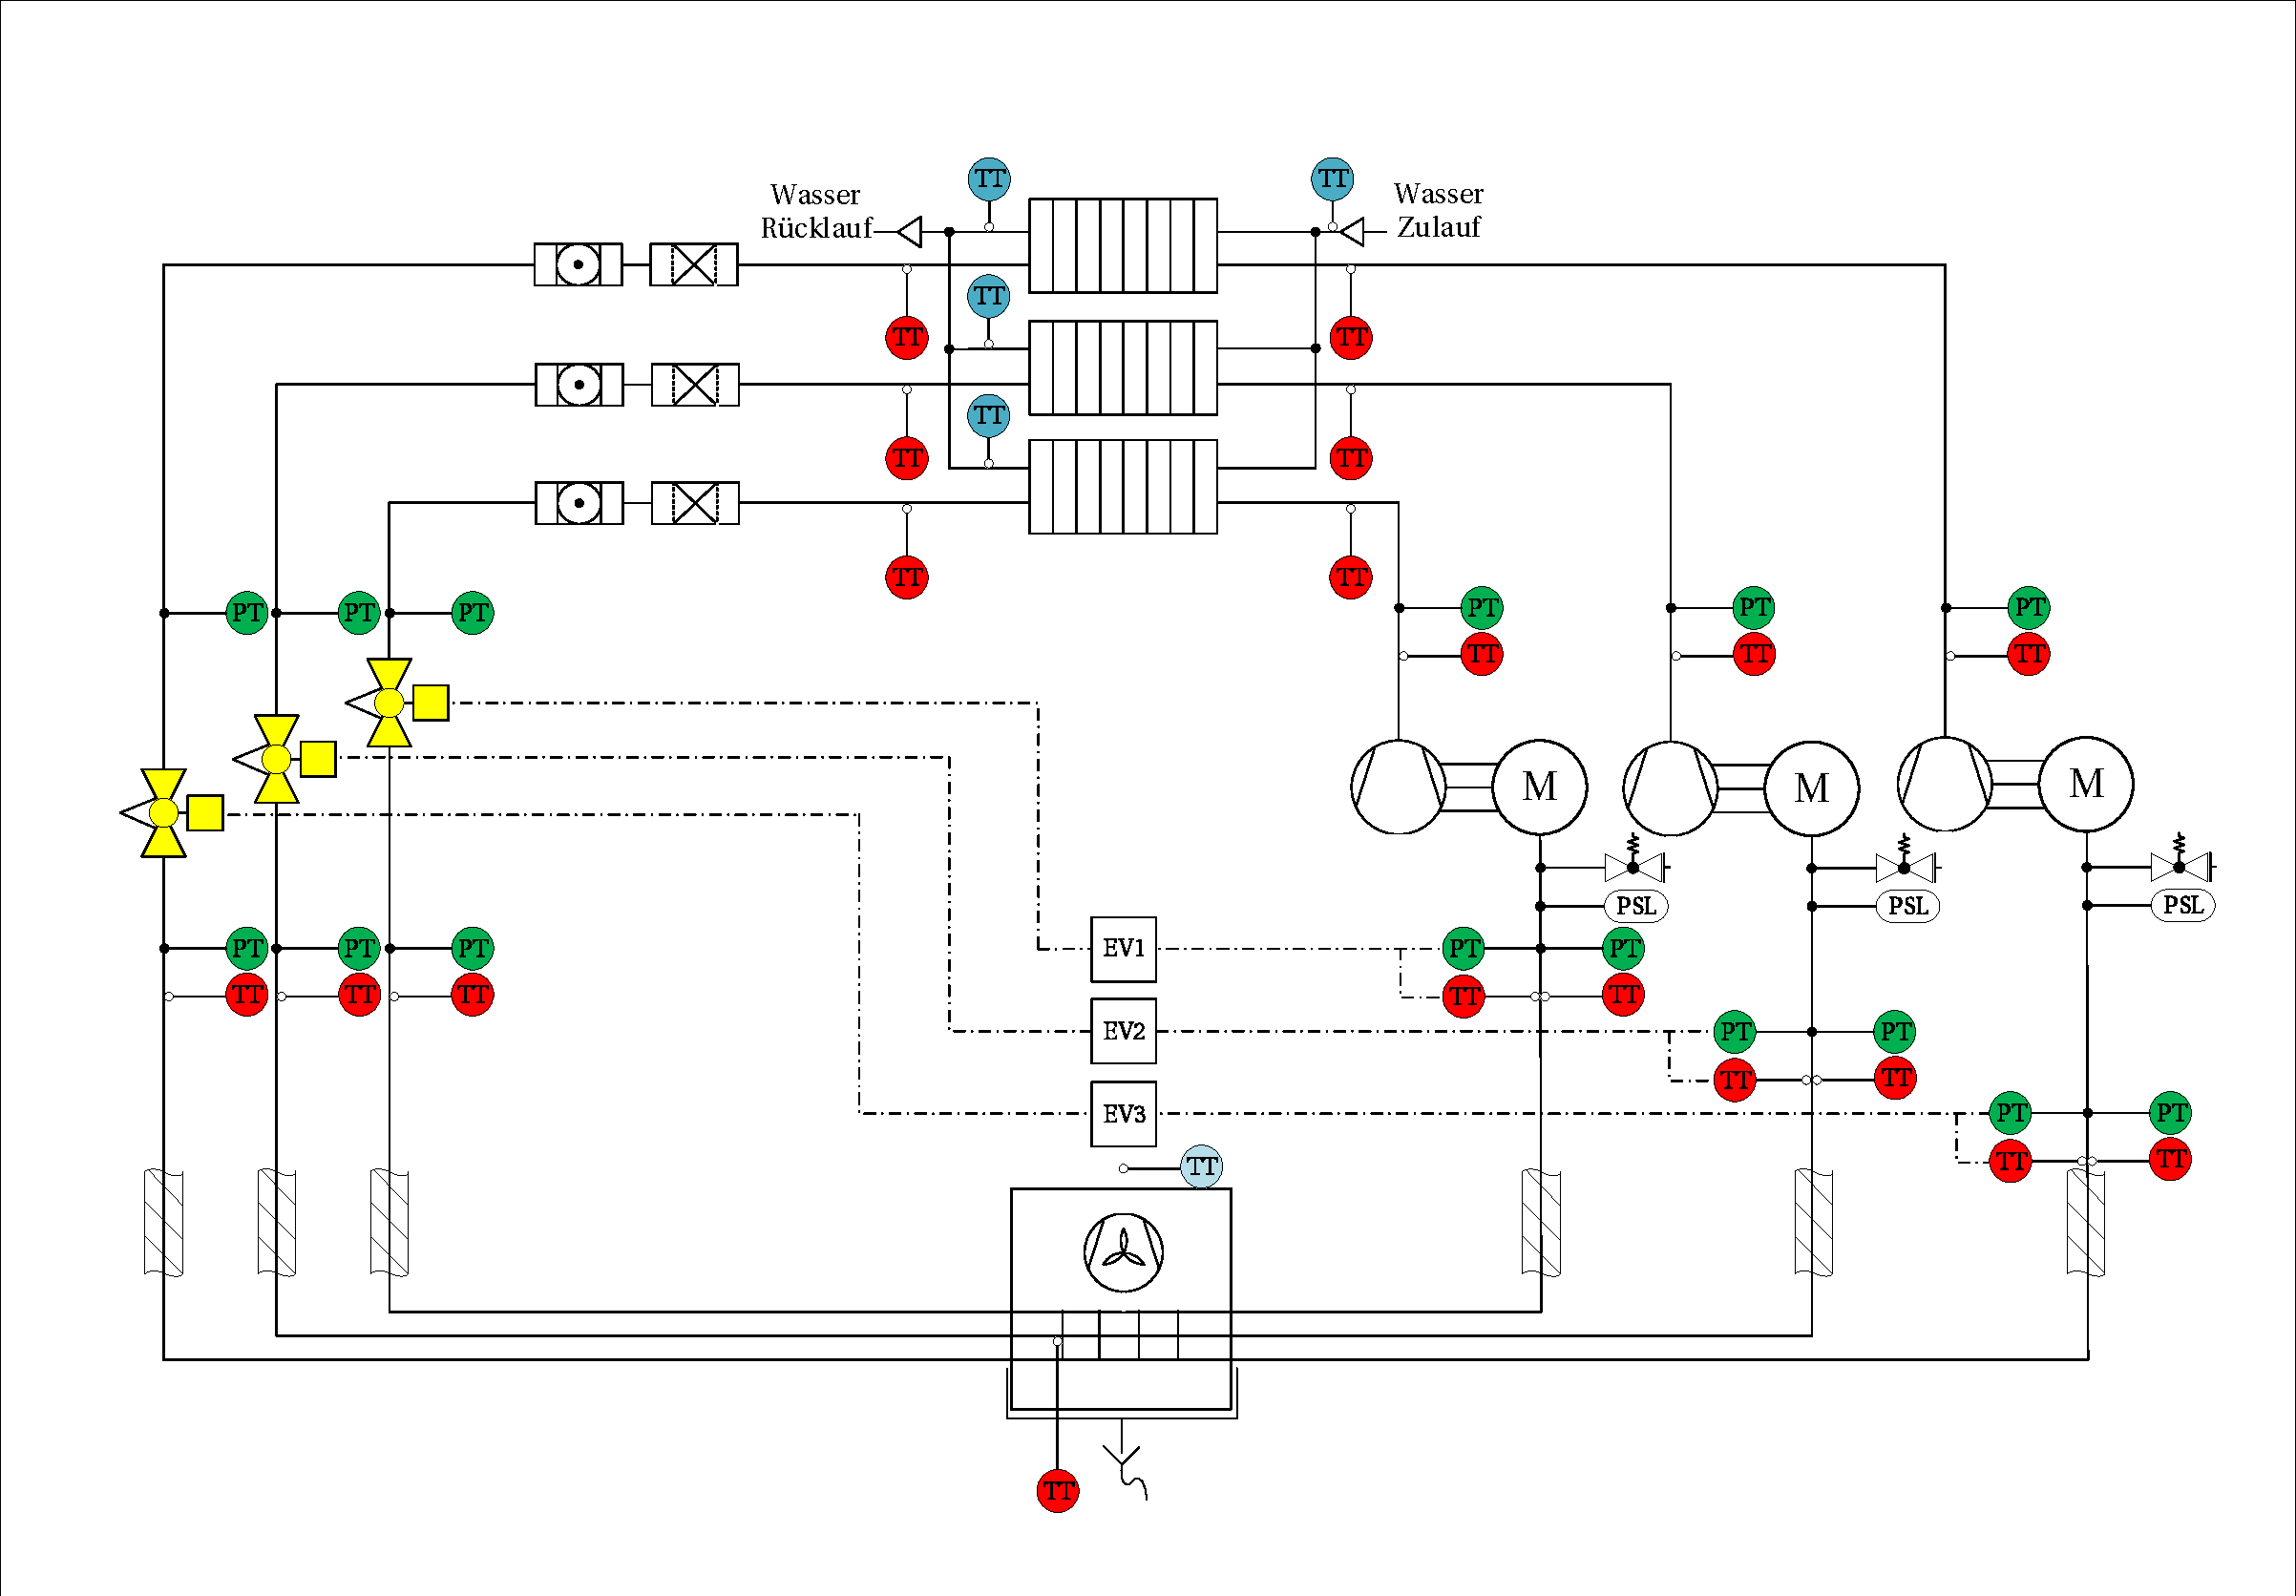
\includegraphics[scale=.56,angle=90]{Pictures/IDC150.pdf}
\caption{Kältekreise des Kühlmöbels.}
\label{fig:IDC150}
\end{figure}


\section{Die Klimakammer}
\label{sec:Die Klimakammer}

In diesem Abschnitt wird der Aufbau und die Funktion der Klimakammer erklärt.
Das Kühlmöbel wird in einer Klimakammer betrieben, um während den Untersuchungen gleichbleibende Umgebungsbedingungen zu generieren und reproduzierbare Ergebnisse zu erzielen.
Abbildung~\ref{fig:Klimakammer} zeigt den Aufbau der Klimakammer und die Position des Kühlmöbels in dieser.
Die Klimakammer besteht aus zwei kleineren Kammern mit eigenständigen Klimaregelungen. Aufgrund der Größe des Regals wurde die Trennwand zwischen den Kammern entfernt. Die Klimatisierung der Raumluft übernimmt dabei die Klimaanlage der Kammer B. Damit die aufbereitete Luft den Raum über dessen gesamte Länge durchströmt, wurde die Ansaugöffnung von Kammer B mit einer Decke, die bis zum Ende des Raums reicht, abgedeckt. Vor den Luftauslassgittern besitzen die Kammern Umlenkbleche. Diese sollen eine gleichmäßige Verteilung des Luftmassenstroms über den Austrittquerschnitt erzielen. Die Klimaanlagen sind in der Lage die angesaugte Raumluft zu kühlen, aufzuheizen sowie zu be- und entfeuchten. Die Regelung findet dabei über einen Computer statt. Mithilfe des Programms LabView, welches eine intuitive Benutzeroberfläche bietet, lässt sich Einfluss auf die Soll-Werte, die Dauer der jeweiligen Untersuchung und die Einstellung der Regelparameter nehmen. 
Jede Kammer besitzt zudem einen Wasseranschluss, dessen Vorlauftemperatur regulierbar ist.
Die Kondensatoren des Kühlregals werden mit temperiertem Wasser der Regelung von Kammer A beaufschlagt. Die Regelung der Kondensationstemperatur wird mittels zwei Pumpen in einem primären und einem sekundären Wasserkreislauf realisiert. Die Pumpe im primären Wasserkreislauf beaufschlagt die Kondensatoren mit Wasser und hält eine Temperaturdifferenz von \unit{5}{\kelvin} über diesen konstant. Die Pumpe des sekundären Wasserkreislaufs regelt über einen Wärmeübertrager zwischen den beiden Kreisen die Temperatur des Wassers am Eintritt des Kondensators auf \unit{35}{\celsius}.


\begin{figure}[htb]
\centering
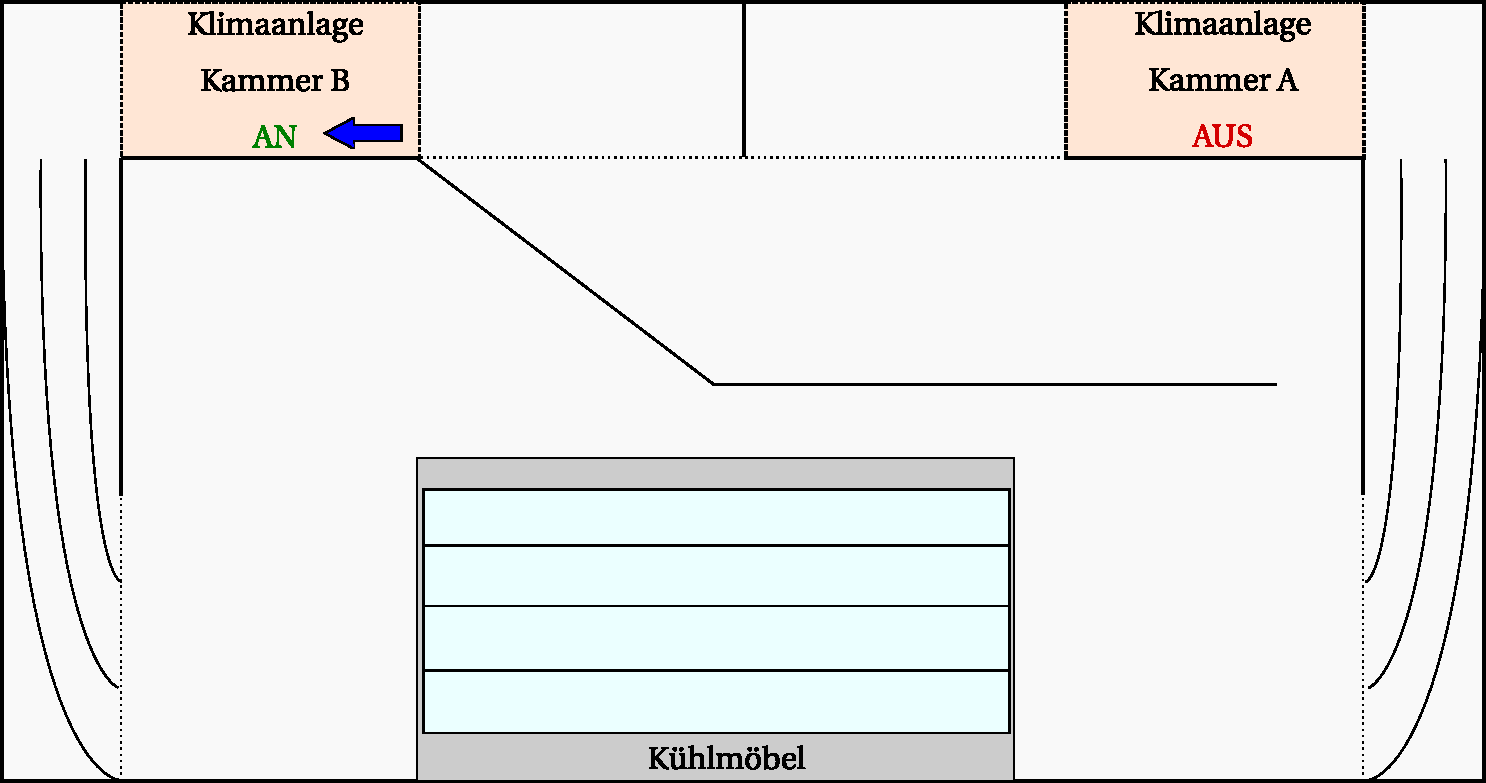
\includegraphics[scale=.6]{Pictures/ClimateChamber.pdf}
\caption{Klimakammer.}
\label{fig:Klimakammer}
\end{figure}

\section{Messdatenerfassung und Berechnungsgrößen}
\label{sec:Erfassung von Messdaten}

Es werden Geräte und Programme verwendet um alle physikalischen Größen während des Betriebs möglichst genau zu erfassen und zu speichern. Insgesamt finden drei Systeme Anwendung um sensorbasiert Daten zu erfassen, umzuwandeln und in Tabellenform zu speichern. Alle erfassten sowie berechneten Messdaten werden über die letzten \unit{75}{\%} des letzten Kühlzyklus in einem Untersuchungszeitraum von \unit{24}{\hour} gemittelt. Dies dient der Vergleichbarkeit.


\subsection{Messdaten des Kühlregals}
\label{subsec:Messdaten der Klimakammer}

Mithilfe des Programms NI SignalExpress werden die Messdaten des Kühlregals und der Kältekreisläufe via Modbus erfasst. Um die Temperaturen zu messen werden Thermoelemente  und um die Drücke zu messen Hochgenauigkeitsdruckaufnehmer verwendet. Die erfassten Messwerte sind die Produkttemperaturen sowie Ein- und Austrittstemperatur der Luft am Verdampfer des Kühlregals, die Temperaturen an verschiedenen Positionen der Kältekreisläufe und die Relativdrücke des Kältemittels im System in Heißgasleitung, Flüssigkeitsleitung, Einspritzleitung und Saugleitung. Die Positionen der Sensoren an den Kältekreisläufen sind aus Abbildung~\ref{fig:IDC150} ersichtlich. Zudem wurde noch die Temperatur des Kältemittels nach jedem einzelnen Durchgang durch den Verdampfer erfasst.
In einem Intervall von \unit{5}{\second} werden die erfassten Daten in eine Exceltabelle geschrieben. SignalExpress erstellt in Echtzeit Graphen der Messwerte. Somit lässt sich das Verhalten des Systems jederzeit beobachten.

\subsection{Messdaten der Klimakammer}
\label{subsec:Messdaten der Klimakammer}

Die in Abschnitt~\ref{sec:Die Klimakammer} vorgestellte Klimakammer wird über LabView gesteuert. Die erfassten Messdaten sind raumluftseitig Ist- und Mittelwerte der Temperaturen sowie die relative Luftfeuchtigkeit. Wasserseitig werden Wassermassenstrom sowie Vor- und Rücklauftemperatur gemessen. 
Die Sensoren, welche die Regelgrößen Temperatur und relative Luftfeuchtigkeit aufnehmen, sind zuluftseitig in der Nähe des Auslassgitters positioniert. Alle Temperatursensoren besitzen eine Messungenauigkeit von $\pm$~\unit{1}{\kelvin}. Die Regelgröße der Temperatur entspricht dem Mittelwert von drei, über die Höhe des Luftauslassgitters verteilten Temperatursensoren. Wird der Betrieb der Klimakammer über das Programm gestartet so wird eine Exceldatei erstellt, in die in einem Intervall von \unit{1}{\second} die erfassten Daten geschrieben werden.



\subsection{Messdaten des Leistungsanalysators}
\label{subsec:Messdaten des Leistungsanalysators}

Um den Zustand des Systems auch elektroseitig zu erfassen wird ein Yokogawa WT3000 Leistungsanalysator verwendet. Dieser ist in der Lage Spannungen und Ströme mit einer Genauigkeit von \unit{0,02}{\%} zu erfassen und daraus Blind-, Wirk- und Scheinleistungen zu berechnen. Die abgenommenen Komponenten sind die einzelnen Verdichter, die Ventilatoren und die restlichen Verbraucher des Kühlregals, wie Licht und Relays.
Das Gerät speichert die erfassten und berechneten Messwerte in Tabellenform auf einem externen Datenspeicher. Die Intevalllänge beträgt hierbei \unit{5}{\second}.


\subsection{Berechnungsgrößen am Kältekreis}
\label{subsec:Berechnungsgrössen}

Auf Basis der mithilfe der Messtechnik erfassten Größen werden Leistungen und Bewertungsgrößen berechnet. Diese ermöglichen es, das Verhalten des Systems zu visualisieren und bewerten zu können.
Der an einem Wärmeübertrager übertragene Wärmestrom lässt sich mit Gleichung~\ref{eq:4} allgemein formulieren.

\begin{equation}
\label{eq:4}
\dot{Q}= kA(T_A - T_B) = \dot{M}_{A}(h_{WÜ,aus} - h_{WÜ,ein})
\end{equation}

Die am Kondensator übertragene Leistung berechnet sich auf Basis der Temperaturen und des Massenstroms des Wassers nach Gleichung~\ref{eq:5}.

\begin{equation}
\label{eq:5}
\dot{Q}_{cd}= \frac{\dot{M}_{W}}{3} c_{p,W} (T_{W,aus} - T_{W,ein})
\end{equation}

Da unter den Testbedingungen nicht immer eine Unterkühlung des Kältemittels und damit ein Verlassen des Zweiphasengebietes stattfindet, wird die Enthalpie am Kondensatoraustritt bzw. am Verdampfereintritt mithilfe der erfassten Messdaten am Kondensatoreintritt und der zuvor berechneten Kondensatorleistung nach Gleichung~\ref{eq:6} berechnet.

\begin{equation}
\label{eq:6}
h_{cd,aus} = h_{cd,ein} - \frac{\dot{Q}_{cd}}{\dot{M}_{KM}}
\end{equation}

Der Kältemittelmassenstrom wird auf Basis der Verdampfungs- und der Verlüssigungstemperatur, sowie vom Hersteller ermittelten Koeffizienten anhand von Gleichung~\ref{eq:7} berechnet.

\begin{align}
\label{eq:7}
	\begin{split}
	\dot{M}_{KM} = &C_0 + C_1*T_{ev,sat} + C_2*T_{cd,sat} + C_3*T_{ev,sat}^2 \\
	&+C_4*T_{ev,sat}*T_{cd,sat} + C_5*T_{cd,sat}^2 + C_6*T_{ev,sat}^3 \\
	&+ C_7*T_{cd,sat}*T_{ev,sat}^2 +C_8*T_{ev,sat}*T_{cd,sat}^2 + C_9*T_{cd,sat}^3
	\end{split}
\end{align}

Somit lässt sich mit Gleichung~\ref{eq:8} die Verdampferleistung bestimmen.

\begin{equation}
\label{eq:8}
\dot{Q}_{ev}= \dot{M}_{KM}(h_{ev,aus} - h_{ev,ein})
\end{equation}

Mit Gleichung~\ref{eq:9} wird die EER-Kennzahl berechnet. Diese setzt den am Verdampfer übertragenen Wärmestrom ins Verhältnis zur aufgenommenen elektrischen Leistung. Dies dient der Bewertung der Effizienz des Systems in einem Betriebspunkt \cite{Muller.2016}.


\begin{equation}
\label{eq:9}
EER = \frac{\dot{Q}_{ev}}{P_{el}}
\end{equation}



\section{Testbedingungen nach Norm}
\label{sec:Testbedingungen nach Norm}

In diesem Abschnitt wird die Herleitung konstanter Prüfbedingung nach Norm erläutert.
Die Norm DIN EN ISO 23953-2 liefert Vorgaben zum Aufbau des Prüfstandes, zur Position der Messtechnik und zu Berechnungsmethoden. Bei allen Tätigkeiten wird sich an dieser orientiert um reproduzierbare sowie vergleichbare Ergebnisse zu erzielen.
Tabelle~\ref{tab:Klimaklassen} zeigt die genormten Klimaklassen mit deren Klassifikation nach Trockenkugeltemperatur, relativer Luftfeuchtigkeit, Taupunkt und dem Wasserdampfgehalt der Luft. Tabelle~\ref{tab:Temperaturklassen} zeigt die Temperaturklassen der M-Pakete mit der jeweils niedrigsten und höchsten erlaubten Temperatur. Rahmenbedingung ist, dass alle Untersuchungen bei Klimaklasse 3 durchgeführt werden. Die erzielten Produkttemperaturen des Kühlmöbels müssen dabei zwischen \unit{5}{\celsius} und \unit{-1}{\celsius} liegen. \newline
Um Kühlgut möglichst genau zu simulieren, werden je \unit{1}{\kilogram} schwere M-Pakete aus Silikon verwendet. Abbildung~\ref{fig:Anordnung der M-Pakete} zeigt die vorgeschriebene Anordnung dieser M-Pakete in den Regalreihen des Kühlmöbels. Die mit einem X gekennzeichneten Pakete werden mit Temperatursensoren versehen.
Der Messpunkt für die Temperatur und die relative Luftfeuchte muss mittig der Länge des Kühlmöbels und \unit{300}{\milli\metre} vor dessen Oberkante liegen. \newline
Voraussetzung für eine normgerechte Messung ist zudem, dass eine Bewegung der Luft vorhanden ist. Abbildung~\ref{fig:Messpunkte} zeigt die vorgeschriebenen Messpunkte für die Erfassung der Luftgeschwindigkeit. Diese muss an den drei Messpunkten auf der Linie A-A in Abbildung~\ref{fig:Messpunkte} zwischen \unit{0,1}{\meter\per\second} und \unit{0,2}{\meter\per\second} liegen \cite{DINDeutschesInstitutfurNormunge.V..}. \newline
Die erfassten Messwerte und die auf deren Basis berechneten Leistungen sowie Bewertungsgrößen werden über die letzten \unit{75}{\%} des letzten Kühlzyklus in einem Untersuchungszeitraum von \unit{24}{\hour} gemittelt.





% Please add the following required packages to your document preamble:
% \usepackage[table,xcdraw]{xcolor}
% If you use beamer only pass "xcolor=table" option, i.e. \documentclass[xcolor=table]{beamer}
\begin{table}[h!]
\centering
\caption{Klimaklassen.}
\label{tab:Klimaklassen}
\begin{tabular}{|c|c|c|c|c|}
\hline
\textbf{\begin{tabular}[c]{@{}c@{}}Klimaklasse des \\ Prüfraums\end{tabular}} & \textbf{\begin{tabular}[c]{@{}c@{}}Trockenkugel-\\ temperatur\end{tabular}} & \textbf{\begin{tabular}[c]{@{}c@{}}Relative \\ Luftfeuchte\end{tabular}} & \textbf{Taupunkt} & \textbf{\begin{tabular}[c]{@{}c@{}}Wasserdampf-\\ gehalt \\ in trockener Luft\end{tabular}} \\
                                                                           & °C                                                                       & \%                                                                       & °C                & g/kg                                                                                        \\ \hline
0                                                                             & 20                                                                          & 50                                                                       & 9,3               & 7,3                                                                                         \\ \hline
1                                                                             & 16                                                                          & 80                                                                       & 12,6              & 9,1                                                                                         \\ \hline
8                                                                             & 23,9                                                                        & 55                                                                       & 14,3              & 10,2                                                                                        \\ \hline
2                                                                             & 22                                                                          & 65                                                                       & 15,2              & 10,8                                                                                        \\ \hline
%\rowcolor[HTML]{FFFe65}
3                                                                             & 25                                                                          & 60                                                                       & 16,7              & 12                                                                                          
\\ \hline
4                                                                             & 30                                                                          & 55                                                                       & 20                & 14,8                                                                                        \\ \hline
5                                                                             & 27                                                                          & 70                                                                       & 21,1              & 15,8                                                                                        \\ \hline
6                                                                             & 40                                                                          & 40                                                                       & 23,9              & 18,8                                                                                        \\ \hline
7                                                                             & 35                                                                          & 75                                                                       & 30                & 27,3                                                                                        \\ \hline
\end{tabular}
\end{table}

\begin{figure}[h!tb]
\centering
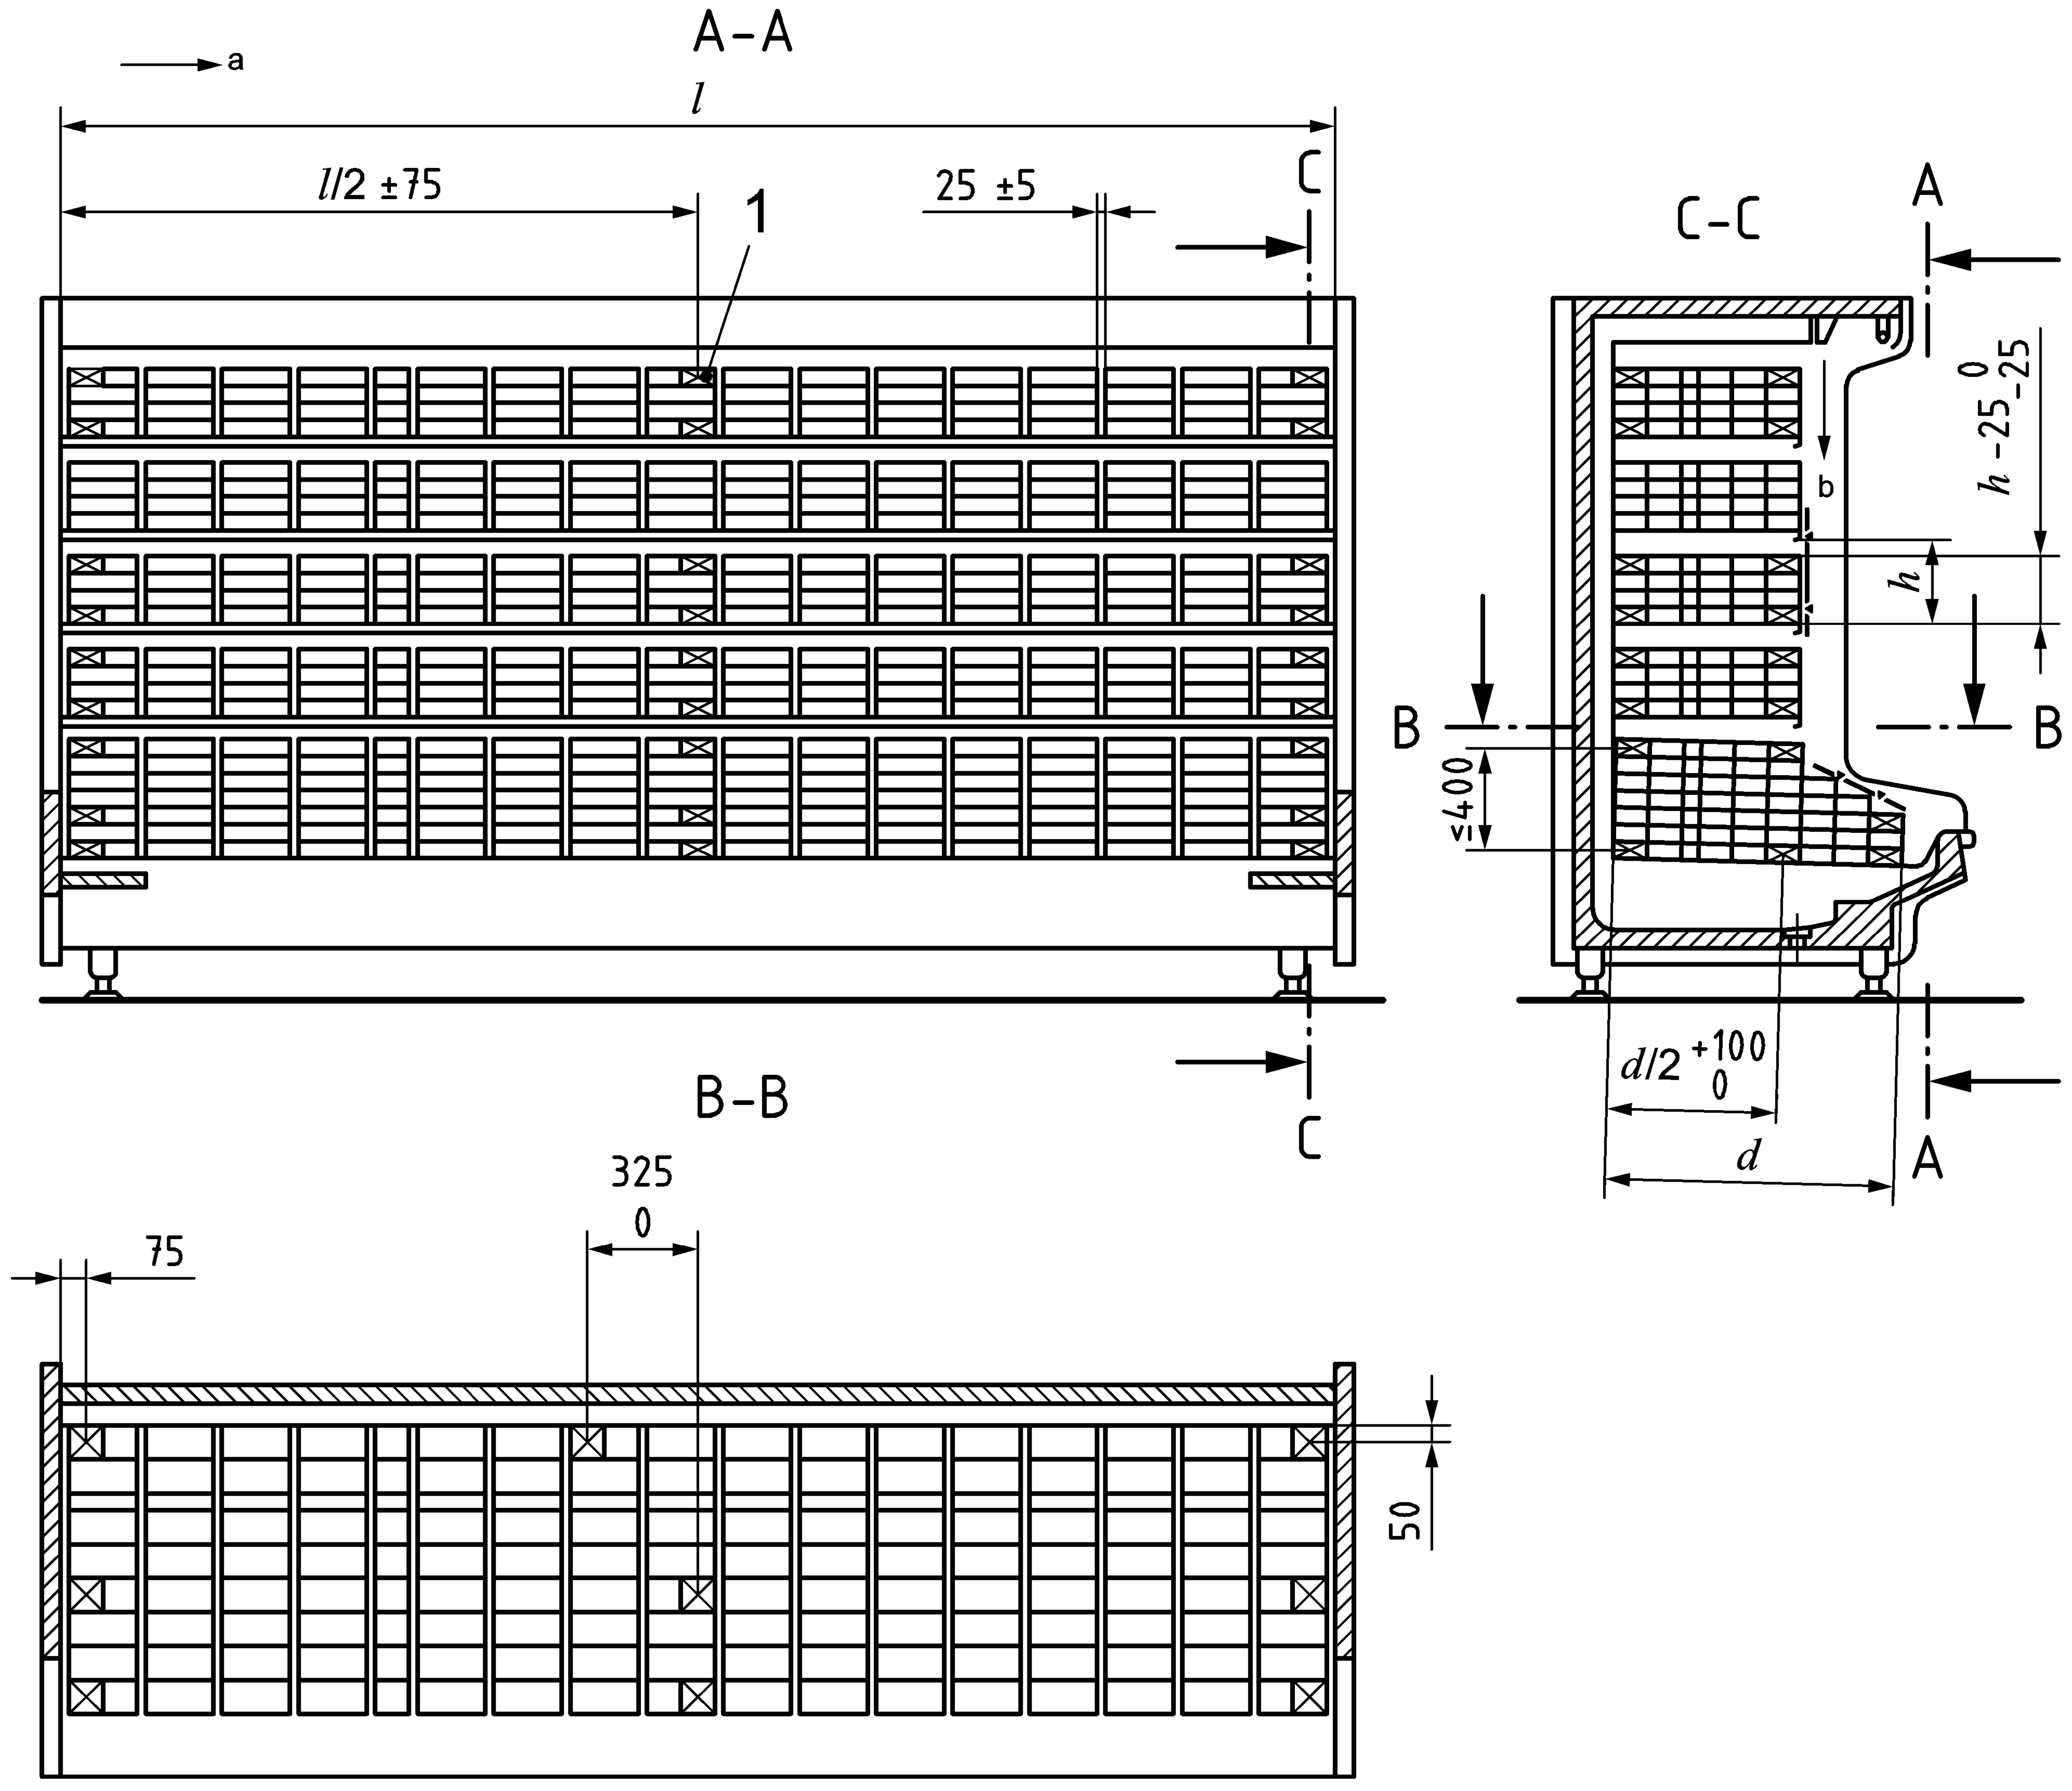
\includegraphics[scale=.12]{Pictures/multi-deck-chilled-cabinet.pdf}
\caption{Anordnung der M-Pakete und der Temperatursensoren.}
\label{fig:Anordnung der M-Pakete}
\end{figure}

% Please add the following required packages to your document preamble:
% \usepackage[table,xcdraw]{xcolor}
% If you use beamer only pass "xcolor=table" option, i.e. \documentclass[xcolor=table]{beamer}
\begin{table}[h!]
\centering
\caption{Temperaturklassen der M-Pakete.}
\label{tab:Temperaturklassen}
\begin{tabular}{|c|c|c|}
\hline
\textbf{Klasse} & \textbf{\begin{tabular}[c]{@{}c@{}}Höchste Temperatur,\\ des wärmsten\\ M-Pakets gleich oder\\ niedriger als\end{tabular}} & \textbf{\begin{tabular}[c]{@{}c@{}}Niedrigste Temperatur,\\ des kältesten\\ M-Pakets gleich oder\\ höher als\end{tabular}} \\ \cline{2-3} 
                & \multicolumn{2}{c|}{°C}                                                                                                                                                                                                                                 \\ \hline
L1              & -15                                                                                                                        & -                                                                                                                          \\ \hline
L2              & -12                                                                                                                        & -                                                                                                                          \\ \hline
L3              & -12                                                                                                                        & -                                                                                                                          \\ \hline
%\rowcolor[HTML]{FFFE65} 
M1              & +5                                                                                                                         & -1                                                                                                                         \\ \hline
M2              & +7                                                                                                                         & -1                                                                                                                         \\ \hline
H1              & +10                                                                                                                        & +1                                                                                                                         \\ \hline
H2              & +10                                                                                                                        & -1                                                                                                                         \\ \hline
S               & \multicolumn{2}{c|}{Sonderklasse}                                                                                                                                                                                                                       \\ \hline
\end{tabular}
\end{table}




\begin{figure}[h!tb]
\centering
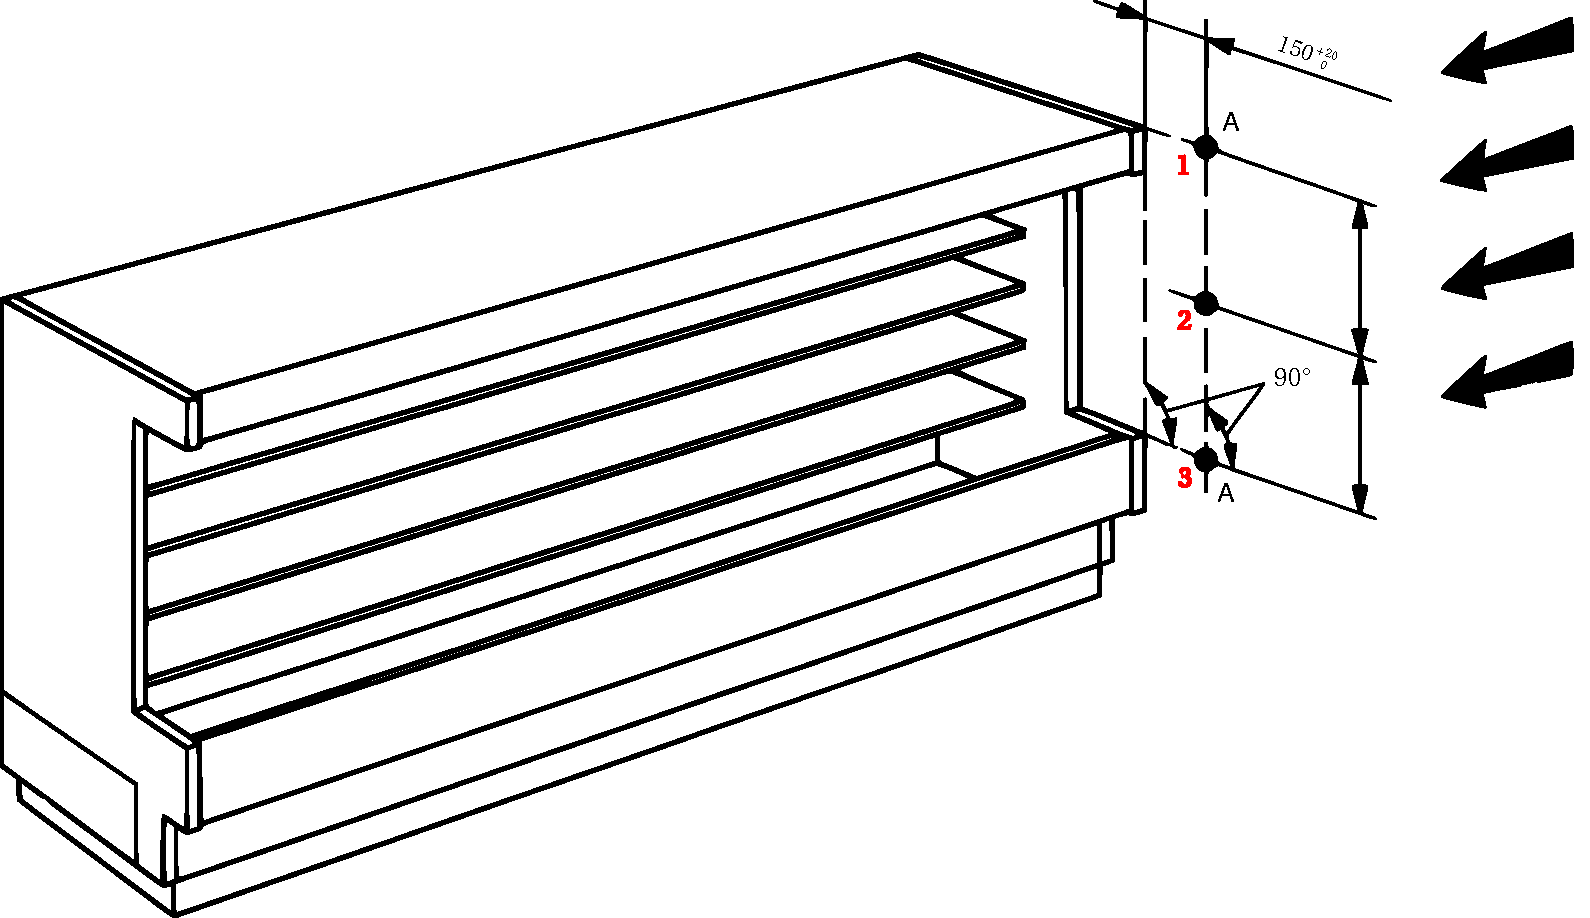
\includegraphics[scale=.5]{Pictures/idc_meas2.pdf}
\caption{Messpunkte.}
\label{fig:Messpunkte}
\end{figure}

\clearpage

\section{Simulationsmodell für Verschaltung der Verdampferrohre}
\label{sec:Simulationsmodell}

In diesem Abschnitt wird das Modellierungsprogramm EES und das zur Beurteilung der Verdampferschaltung erstellte Modell beschrieben und erklärt.
Mithilfe des Programms EES (Engineering Equation Solver) wurde im Rahmen der Untersuchungen ein Modell erstellt, welches es ermöglicht den Effekt einer anderen Verschaltung der kältemittelführenden Leitungen innerhalb des Verdampfers auf dessen Kälteleistung zu simulieren. Grundidee hinter dem Modell ist den, durch den hohen Kältemittelmassenstrom bei gleichzeitig geringem Durchmesser der Verdampferrohre bedingten, Druckabfall und das damit einhergehende Absinken der Sättigungstemperatur zur Erhöhung der Kälteleistung zu nutzen. Im Ausgangsmodell durchströmt das Kältemittel den Verdampfer im Gegenstromprinzip. Aufgrund des Druckabfalls verhält sich diese Anordung wie eine Kombination aus Gleich- und Gegenstrom. Wird nun die Anordnung der Rohre dahingehend geändert, dass das Kältemittel den Verdampfer von dessen Mitte aus im Gleichstrom mit der Luft nach oben durchströmt, die Luft jedoch wie zuvor bei den überhitzten Rohrreihen einströmt, so wird der gegenteilige Effekt erzielt. Der Wärmeübertrager bietet eine Kombination aus Gleich- und Gegenstrom, verhält sich aber wie ein reiner Gegenstromverdampfer. Hierbei ist am Verdampferaustritt der Luft eine höhere Temperaturdifferenz zum Kältemittel zu erwarten. Abbildung~\ref{fig:Vergleich der Verdampferschaltungen} zeigt schematisch für beide Verschaltungen die Reihenfolge, in der das Kältemittel durch den Verdampfer strömt. Die Graphen darunter zeigen die zu erwartenden Temperaturgradienten der Luft und des Kältemittels über die Höhe des Verdampfers. \newline
Das Modell soll zeigen ob diese Maßnahme einen bedeutenden Effekt erzielen kann und wird anschließend im Versuch validiert.


\begin{figure}[htb]
\centering
	\subfigure[Ausgangsschaltung]{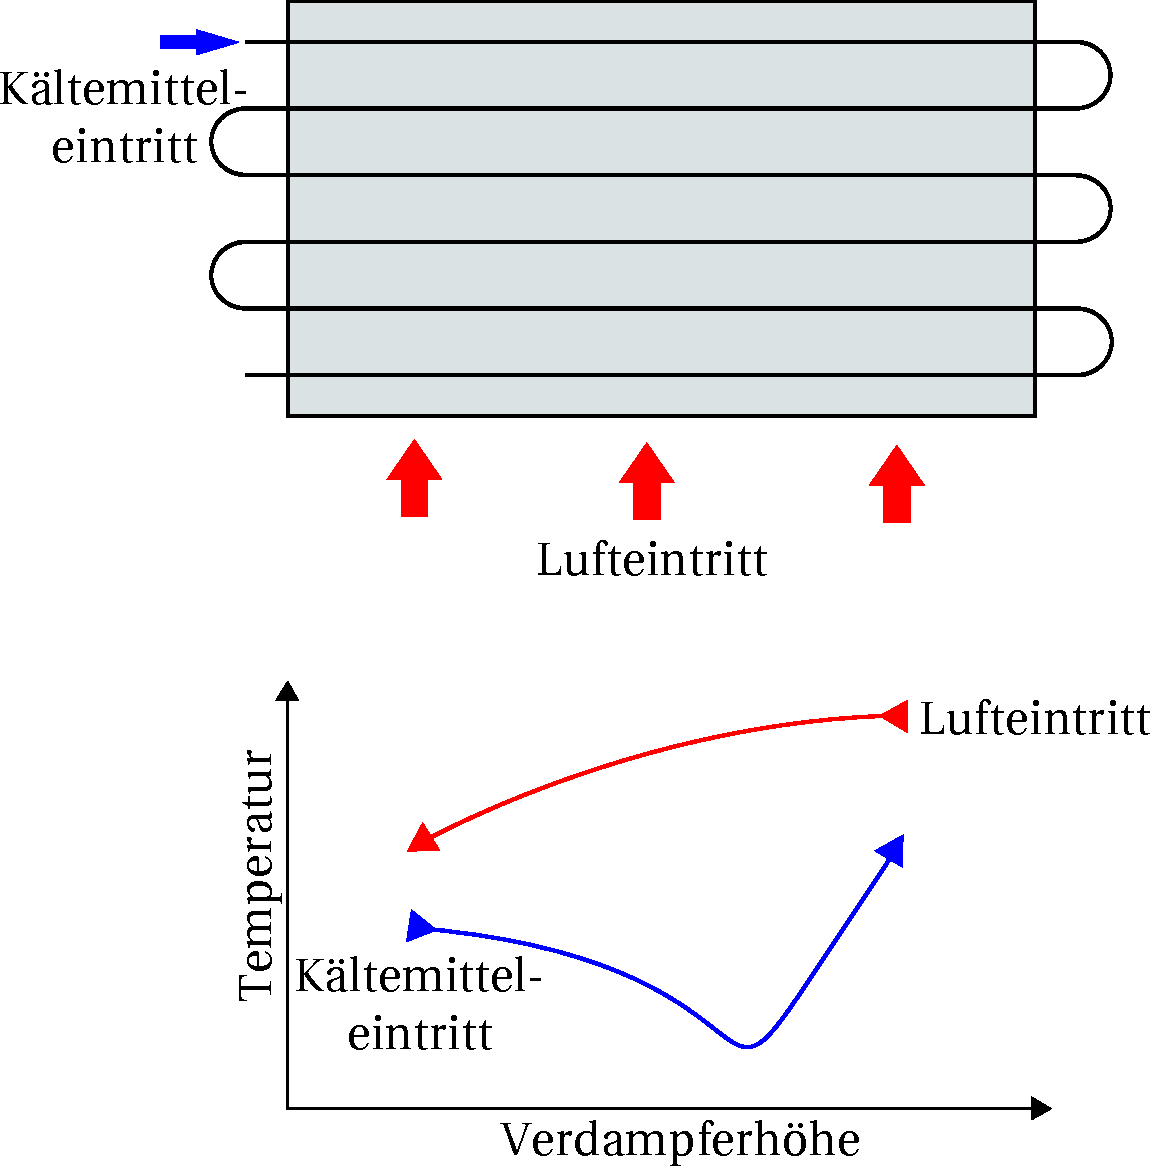
\includegraphics[scale=0.39]{Pictures/Verdampfer_Gegenstrom.pdf}}
	\subfigure[veränderte Schaltung]{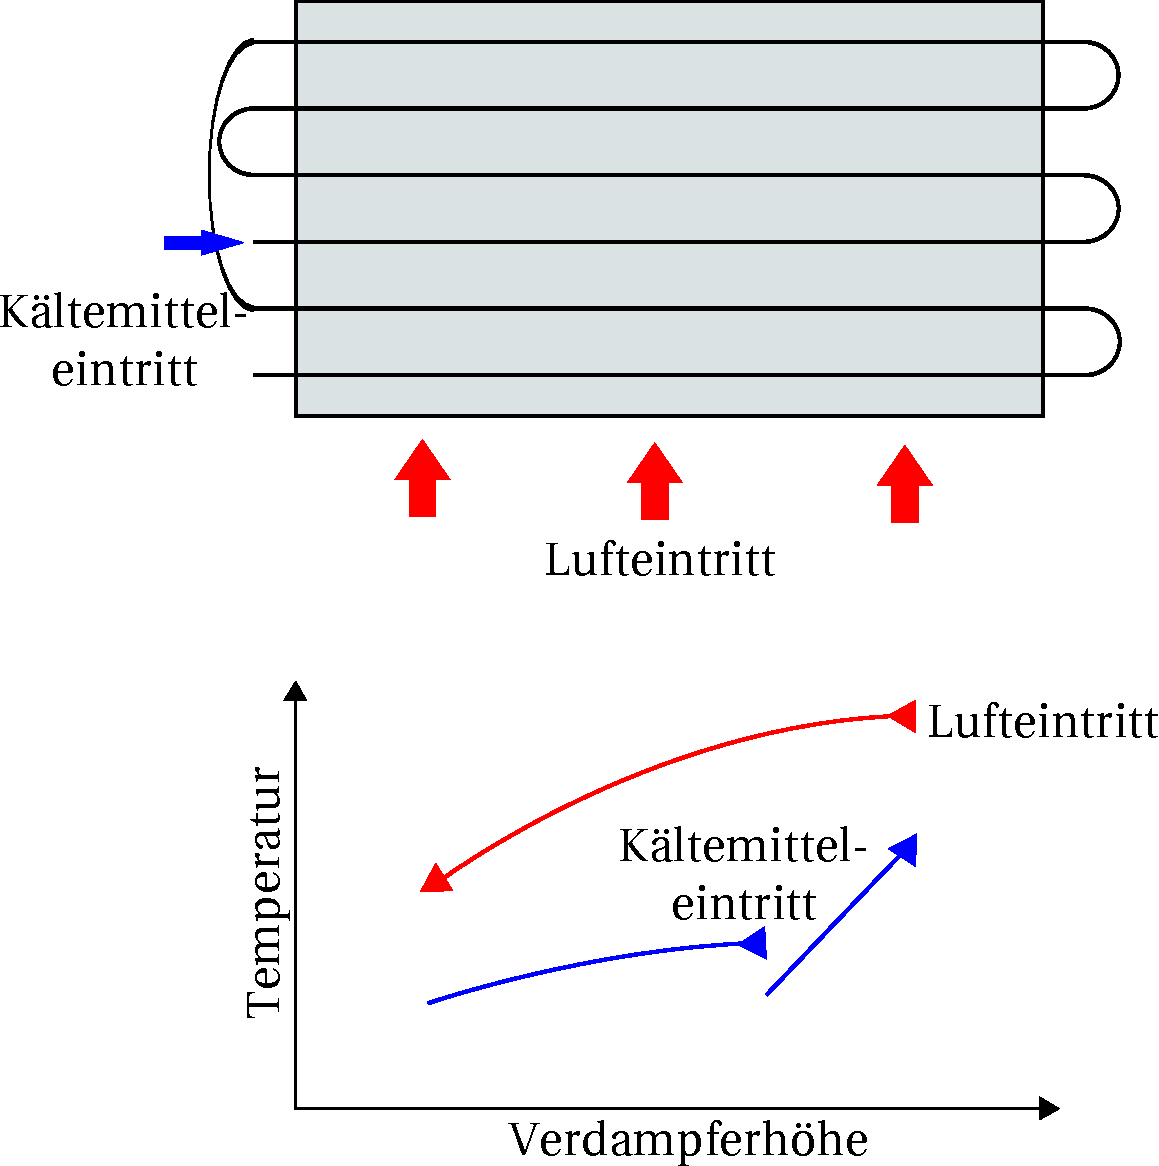
\includegraphics[scale=0.39]{Pictures/Verdampfer_Gleich-Gegenstrom.pdf}}
\caption{Vergleich der Verdampferschaltungen.}
\label{fig:Vergleich der Verdampferschaltungen}
\end{figure}


\subsection{Modellierung mit EES}
\label{subsec:Modellierung mit EES}

EES ist ein Gleichungslöser, der es erlaubt Gleichungen mit Unbekannten unabhängig ihrer Reihenfolge effizient zu lösen. Zudem besitzt EES eine Vielfalt integrierter mathematischer, sowie thermodynamischer und physikalischer Funktionen auf die sich bequem zugreifen lässt \cite{Klein.2000}. Ausschlaggebend für den Entscheid über die Nutzung des Programms ist vorallem die integrierte Stoffdatenbank, welche den Zugriff auf die Daten einer Vielzahl von idealen sowie realen Fluiden erlaubt. Eine objektorientierte Modellierung ist leider nicht ohne Weiteres möglich, wodurch der Entwicklungsaufwand stark erhöht wird. Damit das Programm genaue Ergebnisse liefert ist es nötig, physikalisch sinnvolle und möglichst genaue Begrenzungen der erstellten Variablen anzugeben. 
Weitere Programmfunktionen erlauben die Erstellung einer Benutzeroberfläche sowie die Erstellung von Tabellen und Graphen. Als sehr nützlich erweist sich dabei die Möglichkeit Stoff-Eigenschaftsdiagramme wie z.B. Mollier- oder log-p-h-Diagramme zu erstellen.



\subsection{Berechnung des Druckabfalls in der Zweiphasen-Strömung}
\label{subsec:Berechnung des Druckabfalls in der Zweiphasen-Strömung}

Die Ausgangsberechnung auf der alle weiteren Berechnung basieren, ist die des Druckabfalls innerhalb der Kältemittelströmung.
Nach Gleichung~\ref{eq:10} setzt sich der gesamte Druckabfall $\Delta p$ aus einem Reibungsanteil $\Delta p_{Reibung}$, einem Beschleunigungsanteil $\Delta p_{Beschleunigung}$ und einem statischen Anteil $\Delta p_{statisch}$ zusammen \cite{SpringerVerlagGmbH.2013},\cite{J.MichaelDoster.}:

\begin{equation}
\label{eq:10}
\Delta p =  \Delta p_{Reibung} \pm \Delta p_{statisch} \pm \Delta p_{Beschleunigung}
\end{equation}

Der statische Anteil, sowie der Beschleunigungsanteil sind sehr gering und deshalb vernachlässigbar. Um den durch Reibung bedingten Druckabfall in einem verdampfenden Fluid zu berechnen muss zunächst bestimmt werden ob die Gasphase dispers oder kontinuierlich ist, d.h. ob Gasblasen getrennt und verteilt in der Flüssigkeit transportiert werden oder zusammenhängend strömen \cite{Kesper.1976}. Nach Gleichung~\ref{eq:11} ist der Reibungsanteil des Druckverlustes das Integral der längenbezogenen Druckänderung über die Länge der Verdampferrohres.

\begin{equation}
\label{eq:11}
\Delta p_{Reibung} = \int_{l_1}^{l_2} \left( \frac{dp}{dl} \right)_{Reibung} dl
\end{equation}

\clearpage

Die Gasphase ist dispers, wenn Gleichung~\ref{eq:12} gilt. Hierbei bezeichnet $\beta$ das Verhältnis der Volumenströme der flüssigen Phase $\dot{V}_F$ und der Gasphase $\dot{V}_G$. $x$ ist der Dampfanteil des Kältemittels, $\rho_F$ die Dichte der flüssigen Phase, $\rho_G$ die Dichte der Gasphase und $Fr$ die Froudezahl.

\begin{equation}
\label{eq:12}
\frac{1}{\beta} = \frac{\dot{V}_G}{\dot{V}_F} = \frac{x\rho_F}{(1-x)\rho_G} \leq \frac{12\sqrt{Fr}}{1+\frac{\sqrt{Fr}}{7}}
\end{equation}

Sie wird als kontinuierlich bezeichnet, wenn wenn Gleichung~\ref{eq:13} gilt:

\begin{equation}
\label{eq:13}
\frac{1}{\beta} = \frac{\dot{V}_G}{\dot{V}_F} = \frac{x\rho_F}{(1-x)\rho_G} > \frac{12\sqrt{Fr}}{1+\frac{\sqrt{Fr}}{7}}
\end{equation}

In allen durchgeführten Berechnungen ist die Dampfphase als kontinuierlich zu betrachten, daher wird sich im Rahmen dieser Ausführungen auf die Gleichungen dieser Annahme beschränkt. Der Reibungsdruckabfall wird wesentlich durch einen intensiven Impulsaustausch zwischen den beiden Phasen beeinflusst \cite{Kesper.1976}. In Gleichung~\ref{eq:14} wird die Zweiphasenströmung wie eine Dampfströmung behandelt und der Einfluss der flüssigen Phase durch eine Korrekturgröße $\gamma$ berücksichtigt. Hierbei ist $\dot{m}$ der auf die Rohrquerschnittsfläche bezogene Massenstrom.

\begin{equation}
\label{eq:14}
\left( \frac{dp}{dl} \right)_{Reibung} = \xi_G \frac{\dot{m}^2 x^2}{4\rho_G} \left(\frac{1}{1-\gamma} \right)^2
\end{equation}

$\xi_G$ ist der Reibungsbeiwert und lässt sich mit Gleichung~\ref{eq:15} bestimmen.

\begin{equation}
\label{eq:15}
\frac{1}{\xi_G} = 2\log(Re_G \sqrt{\xi_G})-0.8
\end{equation}

Dafür muss mit Gleichung~\ref{eq:16} die Reynoldszahl der gasförmigen Phase berechnet werden. $\eta_G$ ist die dynamische Viskosität der Gasphase und $d_i$ der Innendurchmesser des Verdampferrohrs \cite{Awad.2012}.

\begin{equation}
\label{eq:16}
Re_G = \frac{\dot{m} x d_i}{\eta_G}
\end{equation}

Die Korrekturgröße $\gamma$ ist als effektive Querschnittsverengung für den Dampfstrom, verursacht durch die Flüssigkeit, zu interpretieren und kann als Versperrungsfaktor bezeichnet werden. Abhängig von den Geschwindigkeiten und den Dichteverhältnissen muss abschnittsweise zwischen verschiedenen Strömungsformen unterschieden werden. Bei kleinen Massenstromdichten ist die Strömung eben und geschichtet. Bei gesteigertem Durchsatz wird sie wellig und es treten Schwalle auf, durch die der Rohrumfang vollständig von Flüssigkeit benetzt ist. Bei noch höheren Durchsätzen wird die Flüssigkeit tropfenförmig im Gaskern mitgerissen. Durch erhebliche Expansionseffekte bei hohen Geschwindigkeiten findet eine Beschleunigung der Gasphase statt und es stellt sich ein Schlupf zwischen den beiden Phasen ein \cite{Kesper.1976}.
Gleichung~\ref{eq:17} ermöglicht die Berechnung der Korrekturgröße $\gamma$.

\begin{equation}
\label{eq:17}
\gamma = \gamma_F(1-E) + \gamma_E E
\end{equation}

Dabei ist der Verperrungsfaktor für ebene Strömung $\gamma_E$. Dieser lässt sich mithilfe von Gleichung~\ref{eq:18} bestimmen.

\begin{equation}
\label{eq:18}
\gamma_E = 1 - \left( 1+0.15 \left( \frac{1-x}{x} \right)^{0.45} \left( \frac{\eta_F}{\eta_G}-1 \right)^{0.25} (1 + 3x^4)\right)^{-1}
\end{equation}


Der Versperrungsfaktor für Ringströmung mit Schwallen $\gamma_F$ lässt sich mit Gleichung~\ref{eq:19} berechnen. $\eta_F$ ist die dynamische Viskosität der flüssigen Phase.

\begin{equation}
\label{eq:19}
\gamma_F = 1 - \left(1+\frac{(1-x)\rho_G}{x \epsilon \rho_F}\right)^{-1.19}
\end{equation}


Gleichung~\ref{eq:20} erlaubt die Berechnung des Verteilparameters $E$. $c_G$ bezeichnet die Schallgeschwindigkeit in der Gasphase.

\begin{equation}
\label{eq:20}
E = 1.857 + 0.815 \log\left[\left(\frac{\dot{m} x}{\rho_G c_G}\right)^2 \left( 1+ \frac{4575 \rho_G^2}{\rho_F^2} \right)\right]
\end{equation}

$E$ darf immer nur Werte zwischen 0 und 1 annehmen. Liegt ein Ergebnis außerhalb dieses Bereichs wird E mithilfe einer Bedingung auf 0 bzw. 1 gesetzt. Bei $E=0$ ist die Strömungsform Ringschwallströmung, bei $E=1$ beschleunigte Strömung.
Für die Berechnung von $\gamma_F$ ist zudem die Berechnung der Hilfsgrößen $\epsilon$ und $\psi$ mithilfe der Gleichungen~\ref{eq:21} bis \ref{eq:24} nötig. $Re_F$ und $Fr_F$ bezeichnen die Reynoldszahl bzw. die Froudezahl der flüssigen Phase.

\begin{equation}
\label{eq:21}
\epsilon^{-3} = \epsilon_1^{-3} + \epsilon_2^{-3}
\end{equation}

mit

\begin{equation}
\label{eq:22}
\epsilon_1 = 1.71 \psi^{0.2} \left( \frac{1-x}{x} \right)^{0.15} \left( \frac{\rho_G}{\rho_F} \right)^{0.5} \left( \frac{\eta_G}{\eta_F} \right)^{0.1}
\end{equation}

und

\begin{equation}
\label{eq:23}
\epsilon_2 = 9.1 \psi
\end{equation}

\clearpage

sowie

\begin{equation}
\label{eq:24}
\psi = (Re_F Fr_F)^{-\frac{1}{6}} \left( \frac{1-x}{x} \right) \left(\frac{\rho_F}{\rho_G} \right)^{-0.9} \left(\frac{\eta_F}{\eta_G} \right)^{-0.5}
\end{equation}

\subsection{Berechnung des Wärmeübergangs}
\label{subsec:Berechnung des Wärmeübergangs}

Die Ausgangsgröße der Temperatur von Luft und Kältemittel nach jeder Zelle wurde mittels der $\epsilon-NTU$-Methode berechnet \cite{SpringerVerlagGmbH.2013},\cite{Bergman.2011},\cite{Nellis.2009}. $NTU$ (dt. Anzahl der Übertragungseinheiten) und $\epsilon$ bezeichnen dimensionslose Kennzahlen. Diese Methode ist ein Verfahren, das oft bei der Auslegung von Wärmetauschern verwendet wird, da es teils schwierige Berechnungsschritte erspart. Zunächst ist es erforderlich den minimalen und maximalen Wärmekapazitätsstrom $\dot{C}_{min}$ und $\dot{C}_{max}$ der beiden Fluide zu bestimmen.
Für den Wärmekapazitätsstrom der Luft gilt Gleichung~\ref{eq:25}.

\begin{equation}
\label{eq:25}
\dot{C}_{min} = \dot{m}_h c_{p,h}
\end{equation} 

Für den Wärmekapazitätsstrom des Kältemittels gilt Gleichung~\ref{eq:26}.

\begin{equation}
\label{eq:26}
\dot{C}_{max} = \dot{m}_k c_{p,k}
\end{equation}
 

Das Wärmekapazitätsverhältnis $C_r$ ist damit nach Gleichung~\ref{eq:27}.
 
\begin{equation}
\label{eq:27}
C_r = \frac{\dot{C}_{min}}{\dot{C}_{max}}
\end{equation}

Zudem ist es notwendig den Wärmedurchgangskoeffizienten $k$ zu berechnen \cite{LehrstuhlfurWarmeundStoffubertragung.}. Dieser setzt sich aus den Wärmeleitwiderständen $W$ der einzelnen Rohrschichten und Übergängen zusammen. Um flexibel bei der Anpassung der Parameter des Modells an die Realität zu sein wurde hierbei auf eine Analogie zu Widerständen in Reihenschaltung aus der Elektrotechnik zurückgegriffen und die wärmeübertragende Fläche $A$ direkt mit einbezogen. Somit gilt nach Gleichung~\ref{eq:UA}:

\begin{equation}
\label{eq:UA}
kA = \frac{1}{W_{L} + W_{Al} + W_{Cu} + W_{KM}}
\end{equation}
 
Die einzelnen Wärmeleitwiderstände lassen sich mithilfe der Gleichungen~\ref{eq:28} bis \ref{eq:31} berechnen.

\begin{equation}
\label{eq:28}
W_L = \frac{1}{\alpha_{L} d_{Al} \pi l}
\end{equation}

\begin{equation}
\label{eq:29}
W_{Al} = \frac{t_{Al}}{\lambda_{Al} d_{Al} \pi l}
\end{equation}

\begin{equation}
\label{eq:30}
W_{Cu} = \frac{t_{Cu}}{\lambda_{Cu} d_{Cu} \pi l}
\end{equation}

\begin{equation}
\label{eq:31}
W_{KM} = \frac{1}{\alpha_{KM} d_{i} \pi l}
\end{equation}

Die Rohrgeometrie ist dabei wie in Abbildung~\ref{fig:Geometrie} dargestellt.
Die Wärmeübergangszahlen werden mit Orientierung am realen Modell bestimmt.

\begin{figure}[h]
\centering
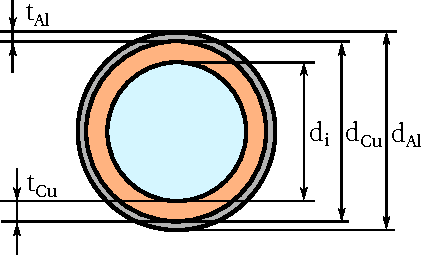
\includegraphics[scale=1]{Pictures/Rohrgeometrie.pdf}
\caption{Geometrie des Verdampferrohres.}
\label{fig:Geometrie}
\end{figure}



Mit diesen Größen lässt sich gemäß Gleichung~\ref{eq:32} der $NTU$-Wert berechnen \cite{McDonald.2012}.

\begin{equation}
\label{eq:32}
NTU = \frac{kA}{\dot{C}_{min}}
\end{equation}

Damit lässt sich die Effektivität des Wärmeübertragers $\epsilon$ bestimmen.
Dabei muss zwischen sensibler und latenter Wärmeaufnahme des Fluids unterschieden werden.
Findet ein Verdampfungsprozess statt so gilt $C_{max}\longrightarrow\infty$ und damit $C_r =0$. Für diesen Fall gilt Gleichung~\ref{eq:33}.

\begin{equation}
\label{eq:33}
\epsilon = 1- \exp{(-NTU)}
\end{equation}

Für den Fall überhitzenden Kältemittels und reinem Kreuzstrom gilt Gleichung~\ref{eq:34}.

\begin{equation}
\label{eq:34}
\epsilon = 1- exp{\left[\left(\frac{1}{C_r}\right)(NTU)^{0.22}(exp{[-C_r(NTU)^{0.78}]}-1)\right]}
\end{equation}

\clearpage

Im Anschluss ist es  möglich den übertragenen Wärmestrom $\dot{Q}$ gemäß Gleichung~\ref{eq:35} zu berechnen. $T_{L,ein}$ bezeichnet die Eintrittstemperatur der Luft in und $T_{KM,ein}$ die Eintrittstemperatur des Kältemittels in die berechnete Zelle.

\begin{equation}
\label{eq:35}
\dot{Q} = \epsilon \dot{C}_{min} (T_{L,ein} - T_{KM,ein})
\end{equation}

Die Eintrittstemperatur des Kältemittels ist die Sättigungstemperatur bei Eingangsdruck. Aus der Energiebilanz in Gleichung~\ref{eq:36} lassen sich dann Kältemittelaustrittsenthalpie $h_{KM,aus}$ sowie Luftaustrittstemperatur $T_{L,aus}$ bestimmen. $\dot{M}$ bezeichnet den Massenstrom des jeweiligen Fluids. Die Eintrittsenthalpie des Kältemittels $h_{KM,ein}$ ist durch Eingangsdruck und Dampfanteil gegeben.

\begin{equation}
\label{eq:36}
\dot{Q} = \dot{M}_{KM} (h_{KM,ein} - h_{KM,aus}) = \dot{M}_{L} c_{p,L}(T_{L,ein} - T_{L,aus})
\end{equation}




\subsection{Das Modell}
\label{subsec:Das Modell}

Mithilfe der Gleichungssysteme aus Abschnitt~\ref{subsec:Berechnung des Druckabfalls in der Zweiphasen-Strömung} und \ref{subsec:Berechnung des Wärmeübergangs} lassen sich, durch Angabe der Eingangswerte Druck, Dampfanteil, Temperatur und Massenstrom des Kältemittels sowie Temperatur und Massenstrom der Luft, Ausgangswerte nach einer definierten Rohrlänge berechnen. Da die Ergebnisse einer Zelle allein von den Eingangswerten abhängig sind, bietet eine Unterteilung in mehrere kleine Zellen eine höhere Genauigkeit. Um Rechenaufwand und Genauigkeit in der Waage zu halten und mit Orientierung am realen Verdampfer wird das Modell entsprechend der Anzahl der Verdampferrohre eines Kältekreises in sechs Berechnungszellen unterteilt \cite{LehrstuhlfurWarmeundStoffubertragung.b}. Jeder einzelnen Zelle wird eine möglichst realistische individuelle Stromführung zugeordnet. Auf diese Weise ergibt sich aus dem Gesamtapparat ein System zusammengeschalteter Einzelapparate \cite{SpringerVerlagGmbH.2013}.
Über die Benutzeroberfläche lässt sich der Zustand beider Fluide nach jeder einzelnen Zelle ablesen und somit mit den Daten des realen Verdampfers vergleichen.
Das Modell ist nur gültig für die Annahme trockener Luft. Da auch in einer Klimakammer \unit{0}{\%} relative Feuchtigkeit schwierig zu erreichen sind, ist eine Abweichung der Ergebnisse zu erwarten. \newline
Bei der Zellenmethode wird die Austauschfläche in Teilbereiche unterteilt, die nacheinander in gleicher oder unterschiedlicher Reihenfolge von beiden Fluidströmen oder Anteilen davon überströmt werden. Jede Teilfläche wird als Fläche eines Einzelapparates aufgefasst mit individuellen Ein- und Austrittstemperaturen beider Fluide. Abbildung~\ref{fig:Zellenmethode} stellt die Modellbildung beider Verschaltungsarten gegenüber. In Verschaltung~V1 sind die Anfangswerte der Luft und des Kältemittels in der ersten und der letzten Zelle vorgegeben, deshalb erfolgt die Berechnung komplett iterativ. In Verschaltung-V2 ist der Rechenaufwand geringer, da die Berechnung der Zellen~2 bis 4 nicht iterativ erfolgt.

\begin{figure}[htb]
\centering
	\subfigure[Verschaltung V1]{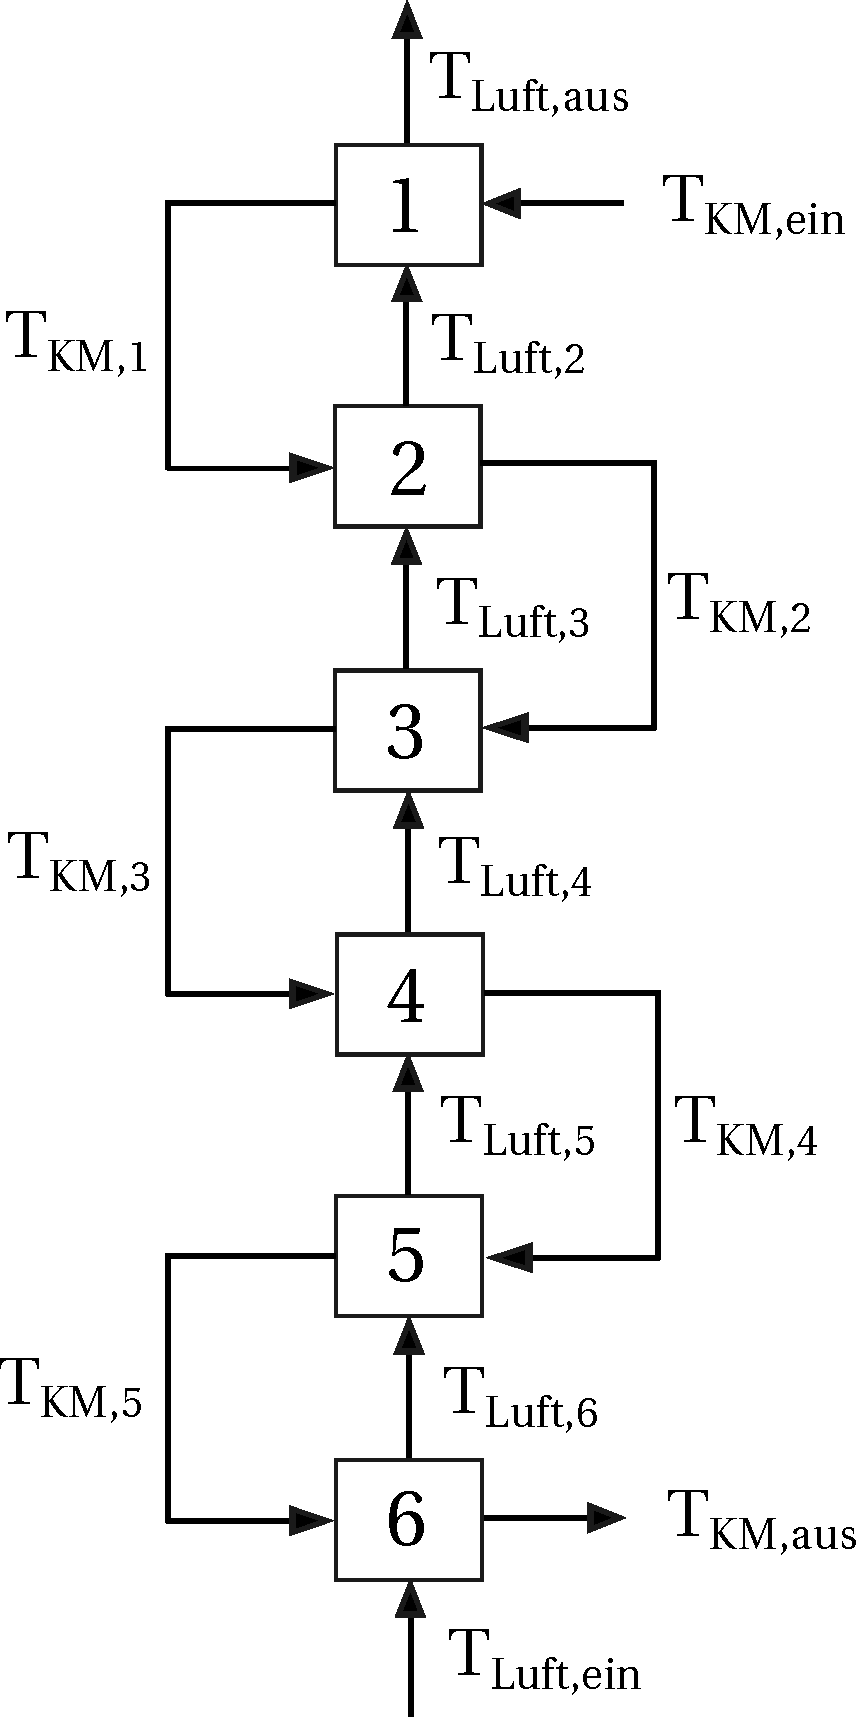
\includegraphics[scale=.5]{Pictures/Verdampfer_V1.pdf}}
	\subfigure[Verschaltung V2]{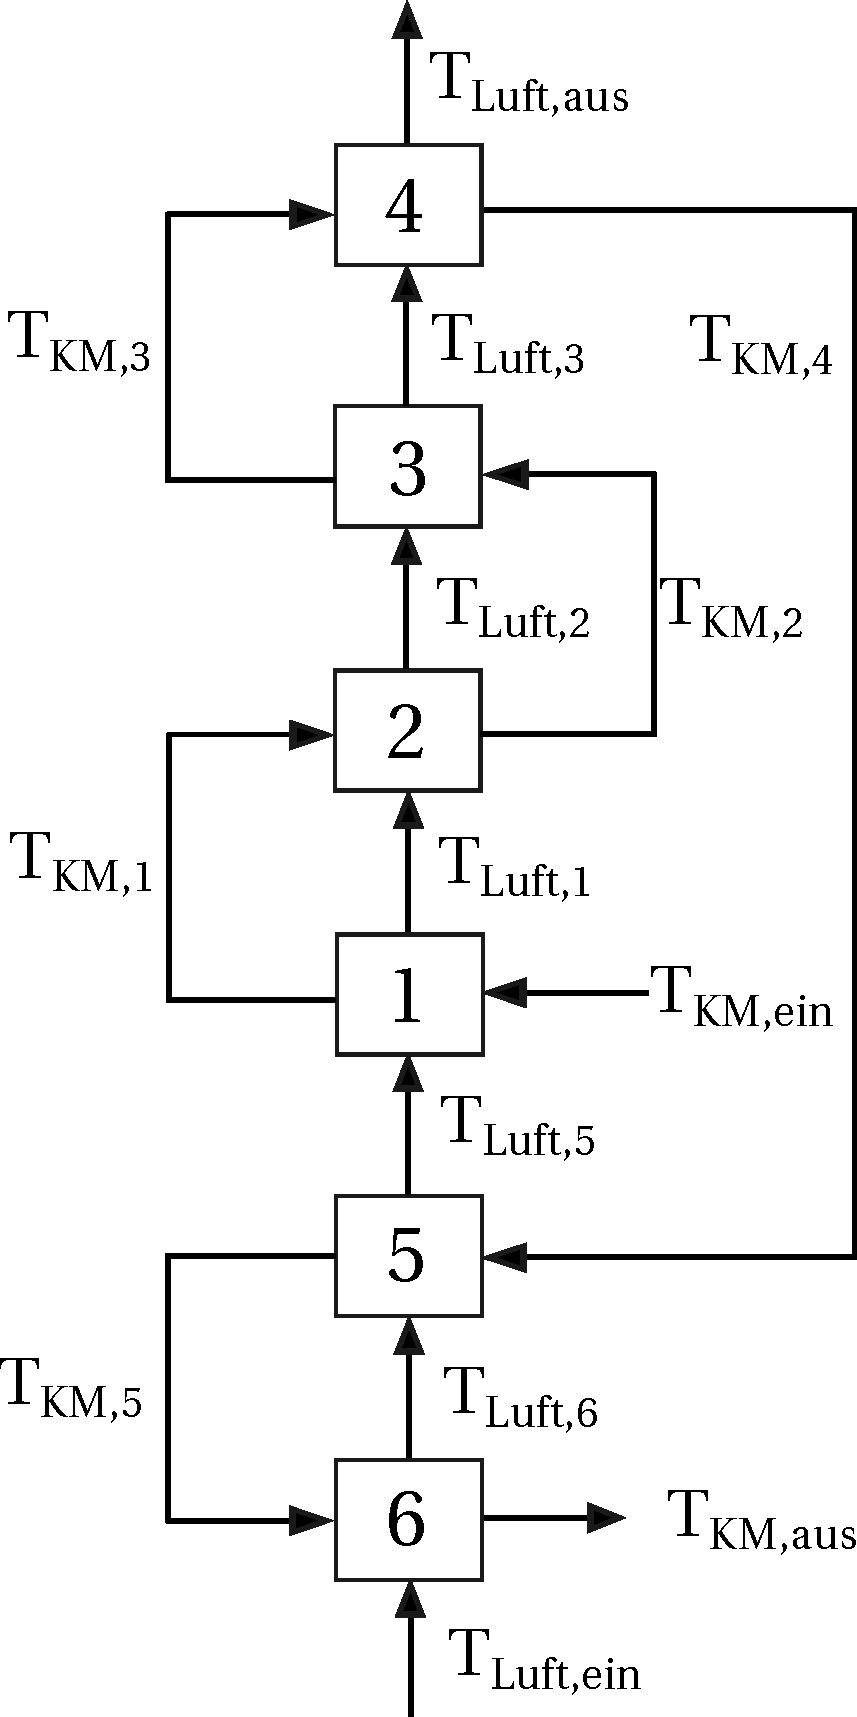
\includegraphics[scale=.5]{Pictures/Verdampfer_V2.pdf}}
\caption{Zellenmethode.}
\label{fig:Zellenmethode}
\end{figure}








%%%%%%%%%%%%%%%%%%%%%%%%%%%%%%%%%%%%%%%%%%%%%%%%%%%%%%%%%%%%%%%%%%%%%%%%%%%%%%%%%%%%%%%%

\chapter{Versuchsdurchführung und Ergebnisse}
\label{cha:Versuchsdurchführung}

In diesem Kapitel wird die Durchführung der Untersuchung sowie die erzielten Ergebnisse beschrieben. Tabelle~\ref{tab:alltests} bietet einen Überblick über die im Rahmen der Arbeit relevanten Untersuchungen.

\begin{table}[h!]
\centering
\caption{Spezifikationen der durchgeführten Untersuchungen.}
\label{tab:alltests}
\begin{tabular}{|ccccccc|}
\hline
Test Nr.              & r. F.                     & Überhitzung              & Öl                               & Abtauintervall          & Verdichter                           & Verdampfer \\ \hline
\multicolumn{1}{|c|}{35} & \multicolumn{1}{c|}{60\%} & \multicolumn{1}{c|}{8K}  & \multicolumn{1}{c|}{3MAF}        & \multicolumn{1}{c|}{4h} & \multicolumn{1}{c|}{ZB09KAU-TFD Hyb} & AHT        \\
\multicolumn{1}{|c|}{50} & \multicolumn{1}{c|}{60\%} & \multicolumn{1}{c|}{8K}  & \multicolumn{1}{c|}{HC~4467} & \multicolumn{1}{c|}{4h} & \multicolumn{1}{c|}{ZB09KAU-TFD Hyb} & AHT        \\
\multicolumn{1}{|c|}{51} & \multicolumn{1}{c|}{60\%} & \multicolumn{1}{c|}{8K}  & \multicolumn{1}{c|}{HC~4467} & \multicolumn{1}{c|}{3h} & \multicolumn{1}{c|}{ZB09KAU-TFD Hyb} & AHT        \\
\multicolumn{1}{|c|}{54} & \multicolumn{1}{c|}{60\%} & \multicolumn{1}{c|}{8K}  & \multicolumn{1}{c|}{HC~4467} & \multicolumn{1}{c|}{3h} & \multicolumn{1}{c|}{ZB09KAU-TFD}     & AHT        \\
\multicolumn{1}{|c|}{58} & \multicolumn{1}{c|}{60\%} & \multicolumn{1}{c|}{8K}  & \multicolumn{1}{c|}{HC~4467} & \multicolumn{1}{c|}{3h} & \multicolumn{1}{c|}{ZB09KAU-TFD}     & LIDL V1    \\
\multicolumn{1}{|c|}{60} & \multicolumn{1}{c|}{60\%} & \multicolumn{1}{c|}{13K} & \multicolumn{1}{c|}{HC~4467} & \multicolumn{1}{c|}{3h} & \multicolumn{1}{c|}{ZB09KAU-TFD}     & LIDL V1    \\
\multicolumn{1}{|c|}{61} & \multicolumn{1}{c|}{0\%}  & \multicolumn{1}{c|}{13K} & \multicolumn{1}{c|}{HC~4467} & \multicolumn{1}{c|}{3h} & \multicolumn{1}{c|}{ZB09KAU-TFD}     & LIDL V1    \\
\multicolumn{1}{|c|}{63} & \multicolumn{1}{c|}{0\%}  & \multicolumn{1}{c|}{13K} & \multicolumn{1}{c|}{HC~4467} & \multicolumn{1}{c|}{3h} & \multicolumn{1}{c|}{ZB09KAU-TFD}     & LIDL V2    \\
\multicolumn{1}{|c|}{64} & \multicolumn{1}{c|}{60\%} & \multicolumn{1}{c|}{13K} & \multicolumn{1}{c|}{HC~4467} & \multicolumn{1}{c|}{3h} & \multicolumn{1}{c|}{ZB09KAU-TFD}     & LIDL V2    \\ \hline
\end{tabular}
\end{table}



\section{Einstellung von Normbedingungen}
\label{sec:EinstellungvonNormbedingungen}

In diesem Abschnitt werden die für die Einstellung von Normbedingungen durchgeführten Untersuchungen beschrieben.
Vor Durchführung der einzelnen Untersuchungen ist es notwendig zu prüfen ob die Umgebungsbedingungen konstant sind und sich an der Norm (siehe Abschnitt~\ref{sec:Testbedingungen nach Norm}) orientieren, um reproduzierbare Ergebnisse zu erzielen. Zu diesem Zweck werden entsprechend Abbildung~\ref{fig:Messpunkte} Sensoren positioniert. Diese zeichnen Temperatur und Geschwindigkeit der Luft über einen Zeitraum von \unit{10}{\min} auf. Mithilfe eines elektrischen Dampferzeugers wird die Luftströmung in der Klimakammer sichtbar gemacht. Damit ist es möglich ein Strömungsbild zu visualisieren und mögliche Ansatzpunkte zum Erreichen der Normbedingungen zu identifizieren. Um die Raumströmung zu verändern werden die Leistung und die Anzahl der laufenden Lüftermotoren über die Kammersteuerungssoftware verändert. Es wird zudem die Öffnung in der abgehangenen Decke verdeckt und geprüft ob dies einen Einfluss auf das Strömungsbild der Luft hat. Dadurch ist die Luft gezwungen entgegen der vorgesehenen Strömungsrichtung durch die abgeschaltete Lüftungsanlage von Kammer A statt nach oben durch die Öffnung in der Decke zu strömen. Die sich als förderlich erwiesenen Änderungen werden anschließend für alle nachfolgenden Untersuchungen angewandt. \newline
Werden die Ergebnisse aller durchgeführten Untersuchungen miteinander verglichen, so lassen sich diese hinsichtlich des Erreichens von Geschwindigkeiten zwischen \unit{0,1}{\meter\per\second} und \unit{0,2}{\meter\per\second} an den drei Messpunkten auf die in Tabelle~\ref{tab:Lüfterleistungen} aufgeführten Untersuchungen eingrenzen. Eine weitere Reduktion der Leistung führt sowohl beim Betrieb mit fünf Lüftern, wie auch mit zwei Lüftern dazu, dass am unteren Messpunkt keine Luftbewegung mehr stattfindet. \

\begin{table}[h!]
\centering
\caption{Genauer betrachtete Untersuchungen zur Ermittlung eines der Norm entsprechenden Betriebspunkts.}
\label{tab:Lüfterleistungen}
\begin{tabular}{|ccc|}
\hline
Lüfteranzahl            & Lüfterleistung          & Decke       \\
{[}Anzahl{]}            & {[}\%{]}                &             \\ \hline
\multicolumn{1}{|c|}{5} & \multicolumn{1}{c|}{10} & offen       \\
\multicolumn{1}{|c|}{5} & \multicolumn{1}{c|}{10} & geschlossen \\
\multicolumn{1}{|c|}{2} & \multicolumn{1}{c|}{30} & offen       \\
\multicolumn{1}{|c|}{2} & \multicolumn{1}{c|}{30} & geschlossen \\ \hline
\end{tabular}
\end{table}

%\begin{table}[h!]
%\centering
%\caption{Untersuchungen zur Ermittlung eines der Norm entsprechenden Betriebspunkts.}
%\label{tab:Lüfterleistungen}
%\begin{tabular}{|ccc|}
%\hline
%Lüfteranzahl            & Lüfterleistung          & Decke       \\
%{[}Anzahl{]}            & {[}\%{]}                &             \\ \hline
%\multicolumn{1}{|c|}{5} & \multicolumn{1}{c|}{8}  & offen       \\
%\multicolumn{1}{|c|}{5} & \multicolumn{1}{c|}{9}  & offen       \\
%\multicolumn{1}{|c|}{5} & \multicolumn{1}{c|}{10} & offen       \\
%\multicolumn{1}{|c|}{5} & \multicolumn{1}{c|}{10} & geschlossen \\
%\multicolumn{1}{|c|}{2} & \multicolumn{1}{c|}{24} & offen       \\
%\multicolumn{1}{|c|}{2} & \multicolumn{1}{c|}{25} & offen       \\
%\multicolumn{1}{|c|}{2} & \multicolumn{1}{c|}{30} & offen       \\
%\multicolumn{1}{|c|}{2} & \multicolumn{1}{c|}{30} & geschlossen \\ \hline
%\end{tabular}
%\end{table}

Die Abbildungen~\ref{fig:10pctOC} - \ref{fig:30pctCC} zeigen den zeitlichen Verlauf der gemessenen Luftgeschwindigkeiten an den Positionen 1 - 3. Auf der y-Achse ist die Luftgeschwindigkeit in $\frac{m}{s}$ abzulesen, auf der x-Achse die Zeit in $h$. Die grünen Markierungen grenzen den Bereich der Luftgeschwindigkeit ein, der durch die Norm vorgeschrieben ist. Die gestrichelten Linien markieren den zeitlichen Mittelwert des jeweiligen Messwertes. \newline
Bei \unit{30}{\%} Lüfterleistung liegen die Geschwindigkeiten an den Messpunkten 1 und 2 über dem Sollwert. Die Geschwindigkeit an Position 3 liegt darunter. Die maximalen Geschwindigkeiten werden an Position 2, auf mittlerer Höhe des Kühlmöbels, gemessen. Diese betragen \unit{0.35}{\metre\per\second} bei offener Decke und \unit{0.3}{\metre\per\second} bei geschlossener Decke. 
Bei \unit{10}{\%} Lüfterleistung liegt der Mittelwert der gemessenen Geschwindigkeit an Position 2 immer innerhalb des vorgeschriebenen Bereichs. Die Geschwindigkeit an Position 1 liegt darüber, die Geschwindigkeit an Position 3 darunter. Die maximalen Geschwindigkeiten betragen \unit{0.35}{\metre\per\second} bei offener Decke und \unit{0.3}{\metre\per\second} bei geschlossener Decke und werden an Position 1 gemessen. \newline
Abbildungen~\ref{fig:10pctOC_temp} und \ref{fig:30pctOC_temp} stellen jeweils den zeitlichen Verlauf der Lufttemperatur an den Positionen 1 - 3 während der Untersuchungen mit \unit{10}{\%} und \unit{30}{\%} Lüfterleistung bei offener Decke dar.
Während die Temperatur an den Positionen 1 und 2 circa im angestrebten Bereich um \unit{25}{\celsius} liegt ist auffällig, dass die Temperatur in Position 3 nach unten abweicht. Beim Betrieb mit \unit{10}{\%} Lüfterleistung ist die Abweichung mit \unit{7}{\kelvin} sehr groß. Bei \unit{30}{\%} Lüfterleistung ist diese nur \unit{1.5}{\kelvin} groß. \newline
Die Abbildungen~\ref{fig:Klimakammer_offeneDecke} und \ref{fig:Klimakammer_geschlosseneDecke} visualisieren den Strömungsverlauf der Luft in der Kammer. Die roten Pfeile stellen dabei eine sichtbare Luftbewegung dar.
Bei geöffneter Decke ist zu erkennen, dass die Luft quer über das Kühlmöbel Richtung Deckenöffung strömt. Bei geschlossener Decke ist der Strömungsverlauf parallel zum Kühlmöbel.




\begin{figure}[h!tb]
\centering
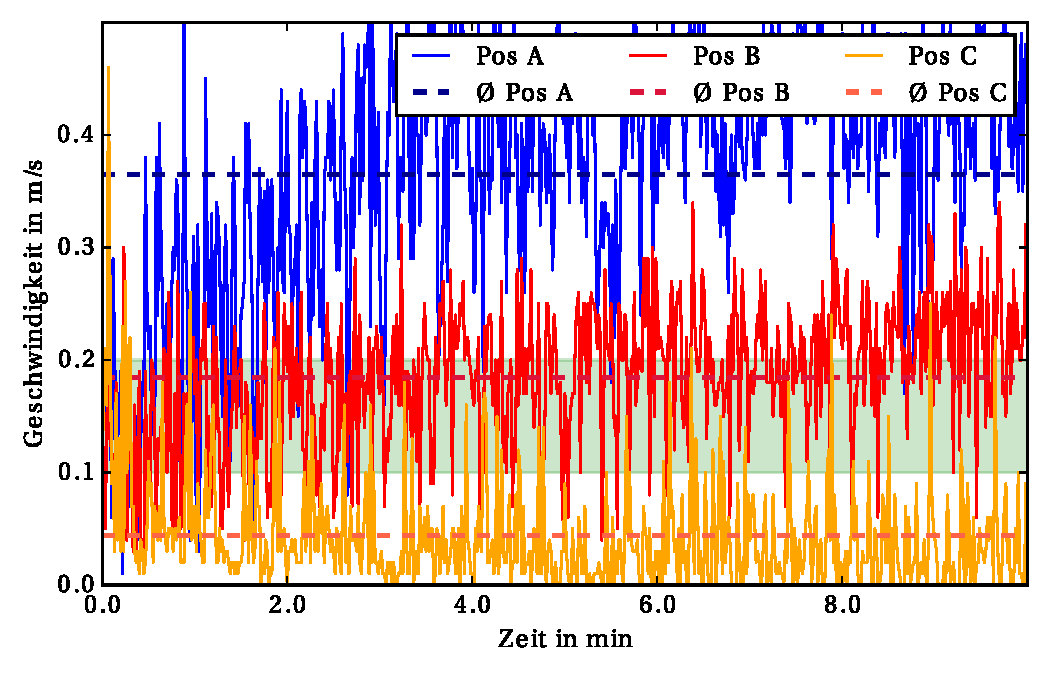
\includegraphics[scale=.8]{Pictures/AV10pctOC1.pdf}
\caption{Luftgeschwindigkeiten bei 10\% Lüfterleistung und offener Decke.}
\label{fig:10pctOC}
\end{figure}


\begin{figure}[h!tb]
\centering
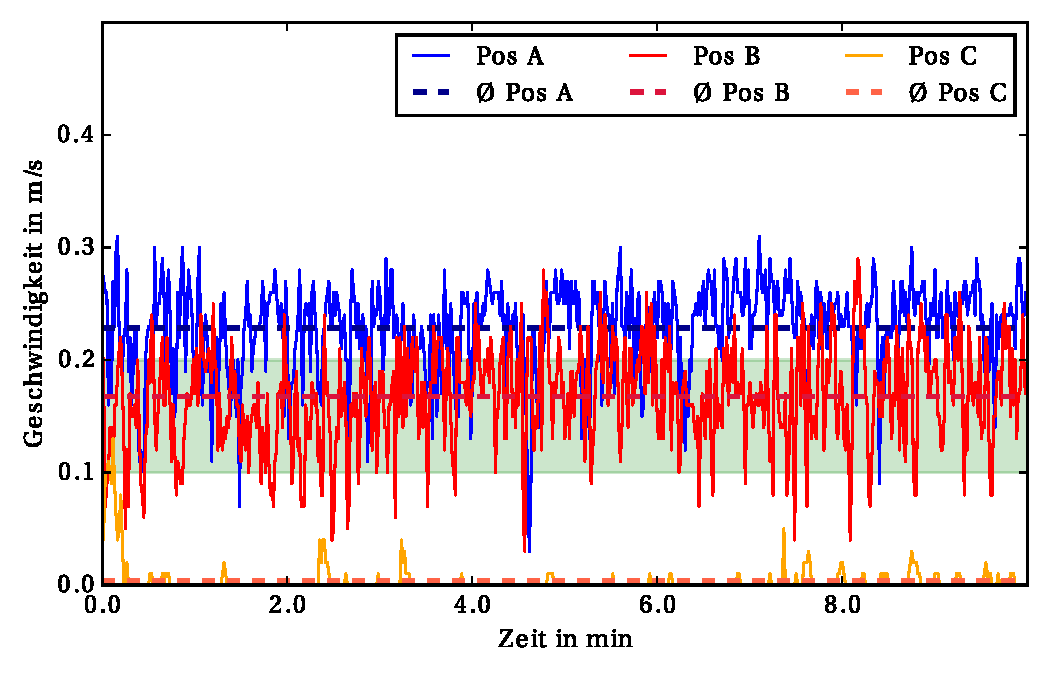
\includegraphics[scale=.8]{Pictures/AV10pctCC1.pdf}
\caption{Luftgeschwindigkeiten bei 10\% Lüfterleistung und geschlossener Decke.}
\label{fig:10pctCC}
\end{figure}


\begin{figure}[h!tb]
\centering
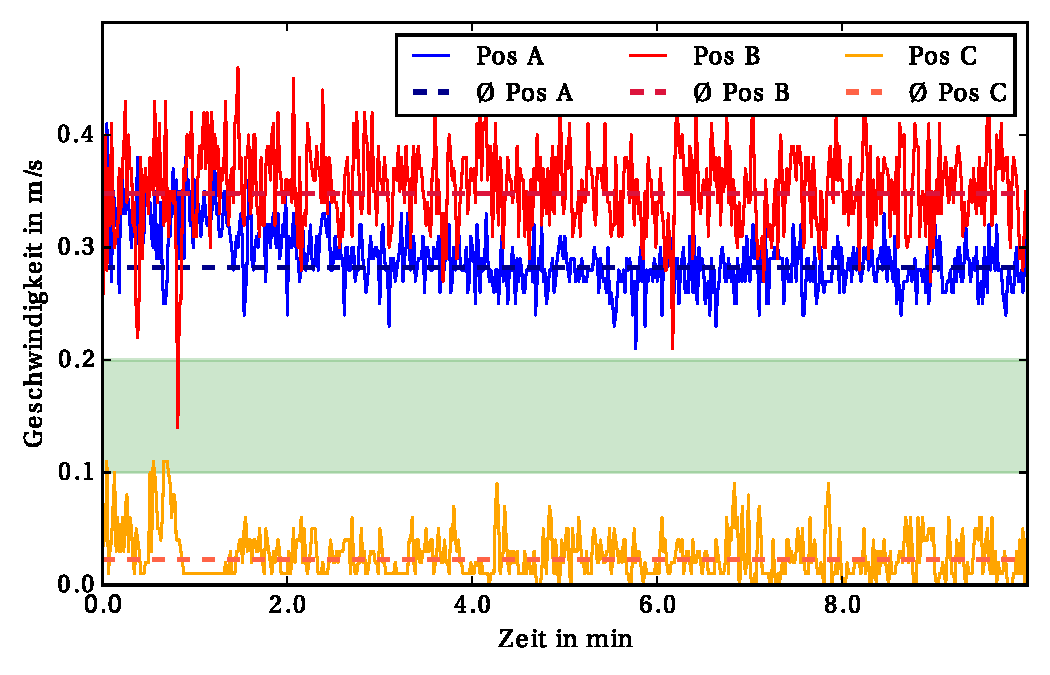
\includegraphics[scale=.8]{Pictures/AV30pctOC1.pdf}
\caption{Luftgeschwindigkeiten bei 30\% Lüfterleistung und offener Decke.}
\label{fig:30pctOC}
\end{figure}


\begin{figure}[h!tb]
\centering
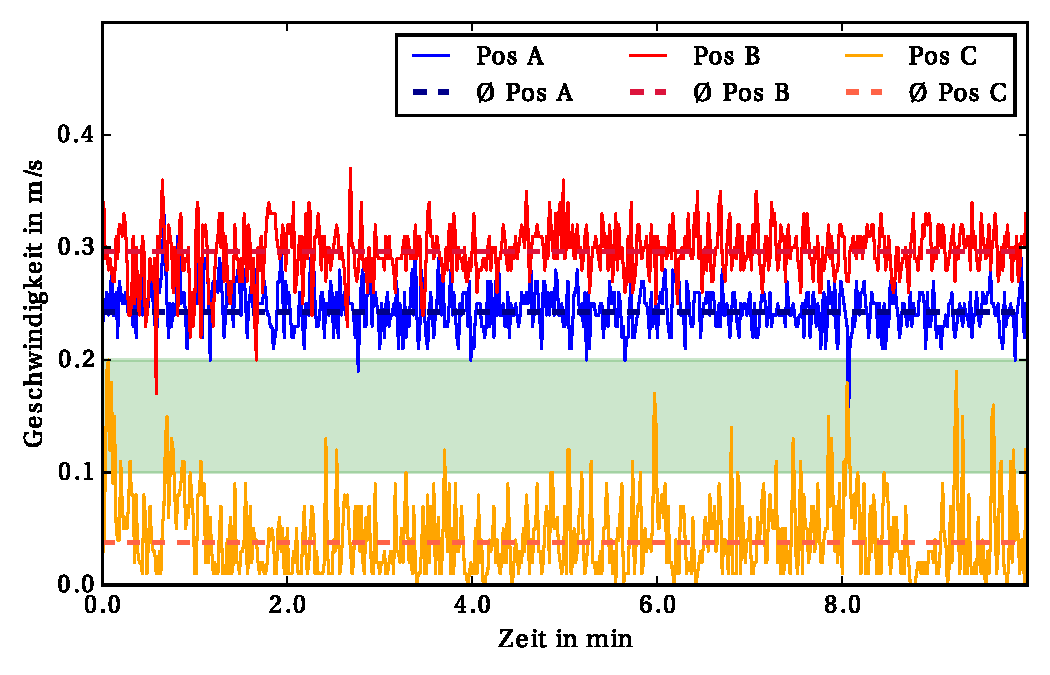
\includegraphics[scale=.8]{Pictures/AV30pctCC1.pdf}
\caption{Luftgeschwindigkeiten bei 30\% Lüfterleistung und geschlossener Decke.}
\label{fig:30pctCC}
\end{figure}

\begin{figure}[h!tb]
\centering
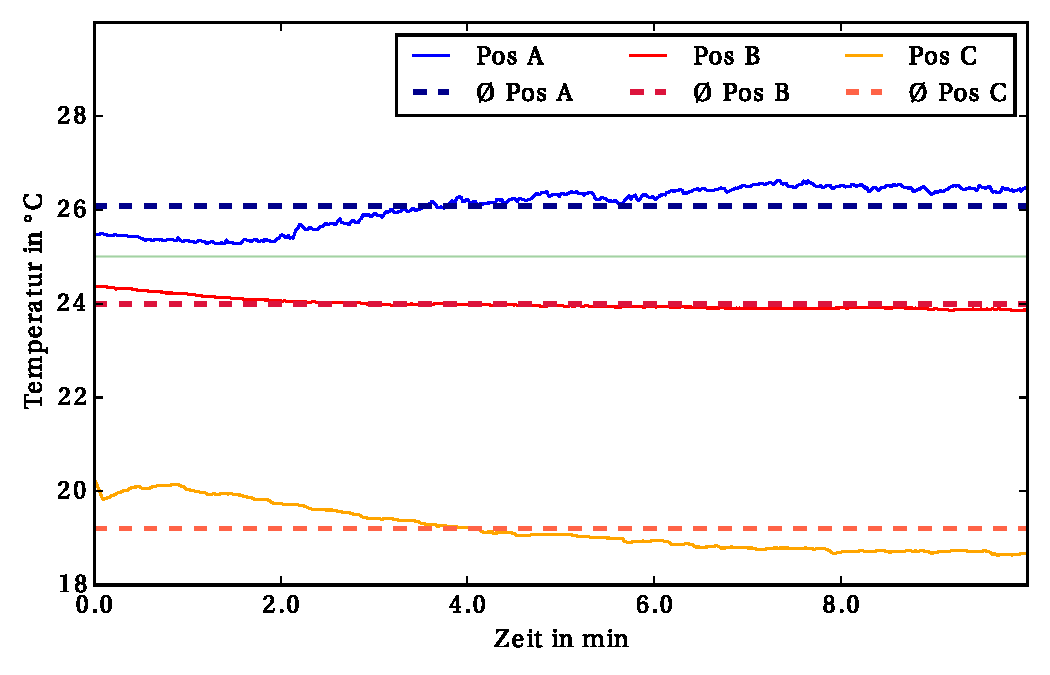
\includegraphics[scale=.8]{Pictures/AT10pctOC1.pdf}
\caption{Lufttemperaturen bei 10\% Lüfterleistung und offener Decke.}
\label{fig:10pctOC_temp}
\end{figure}


\begin{figure}[h!tb]
\centering
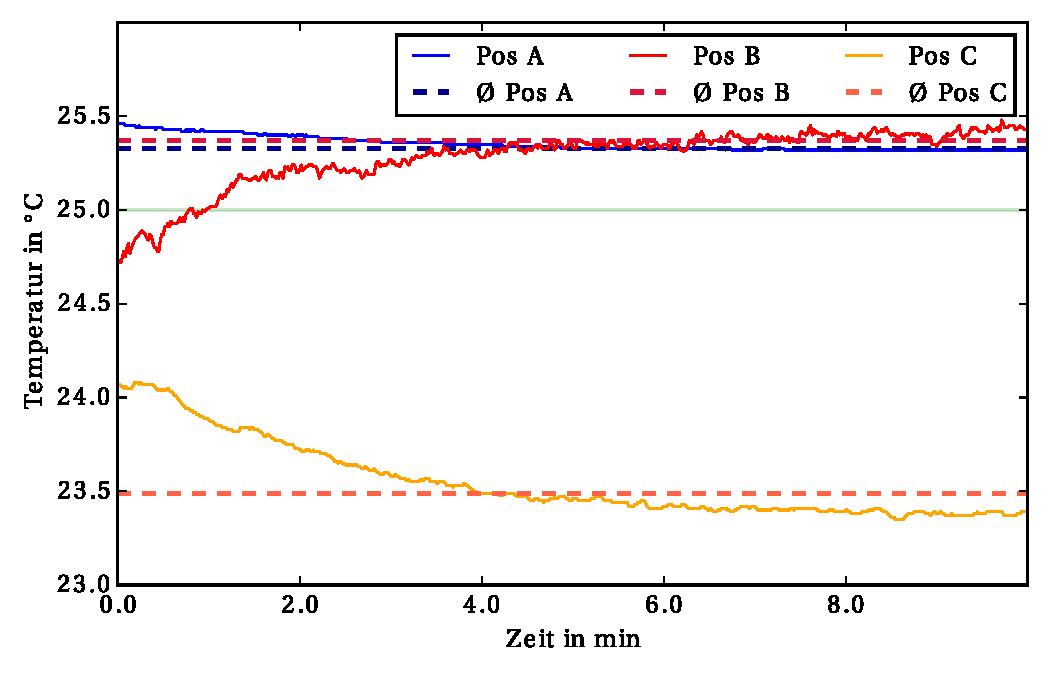
\includegraphics[scale=.8]{Pictures/AT30pctOC1.pdf}
\caption{Lufttemperaturen bei 30\% Lüfterleistung und offener Decke.}
\label{fig:30pctOC_temp}
\end{figure}

\begin{figure}[h!tb]
\centering
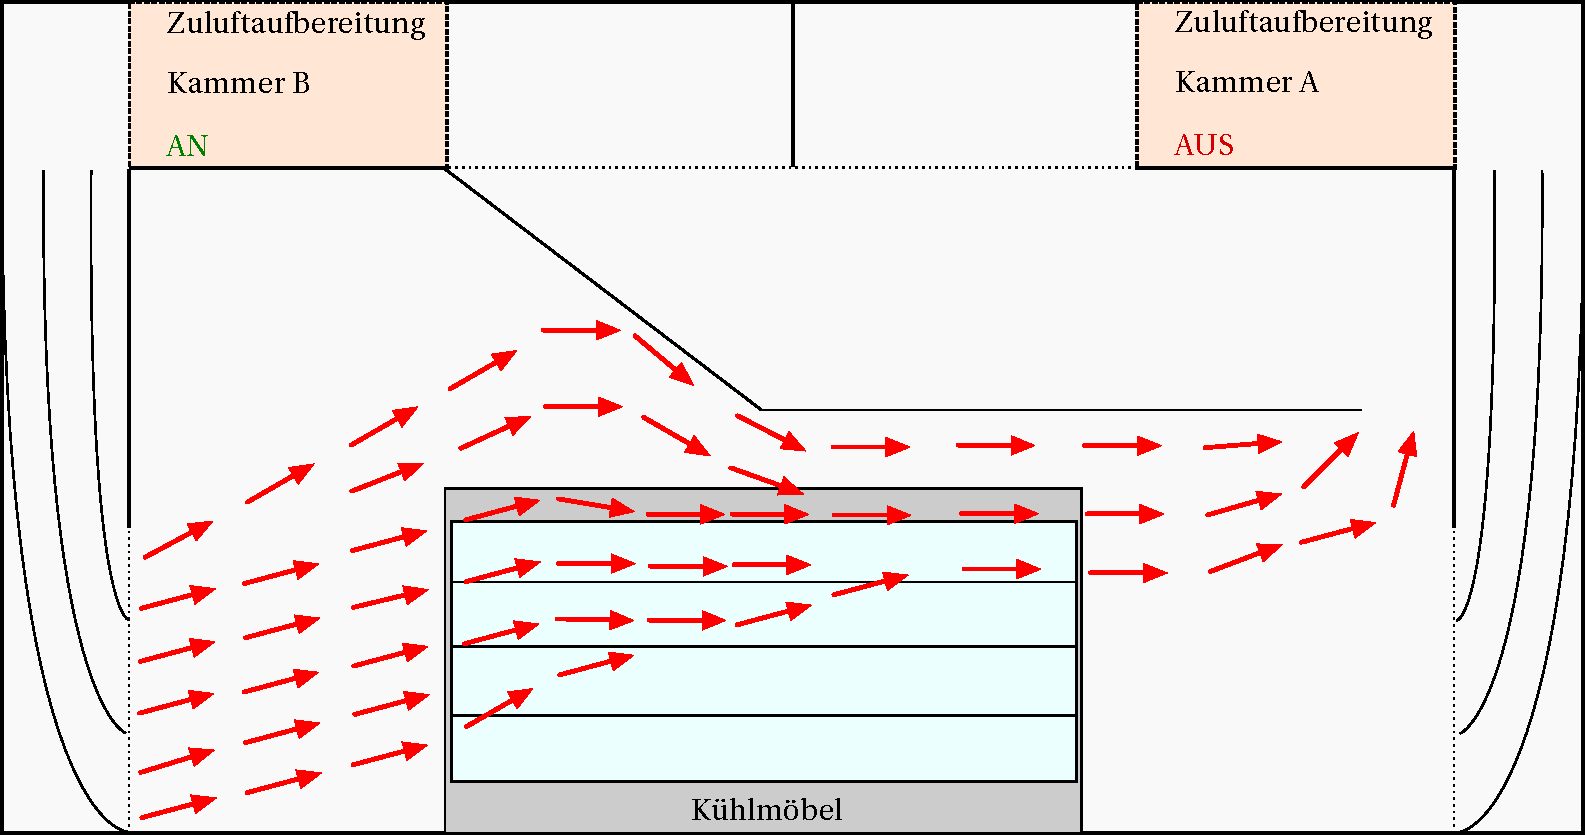
\includegraphics[scale=.6]{Pictures/ClimateChamber_flow30pctOC.pdf}
\caption{Luftströmung in der Klimakammer mit Deckenöffnung.}
\label{fig:Klimakammer_offeneDecke}
\end{figure}

\begin{figure}[h!tb]
\centering
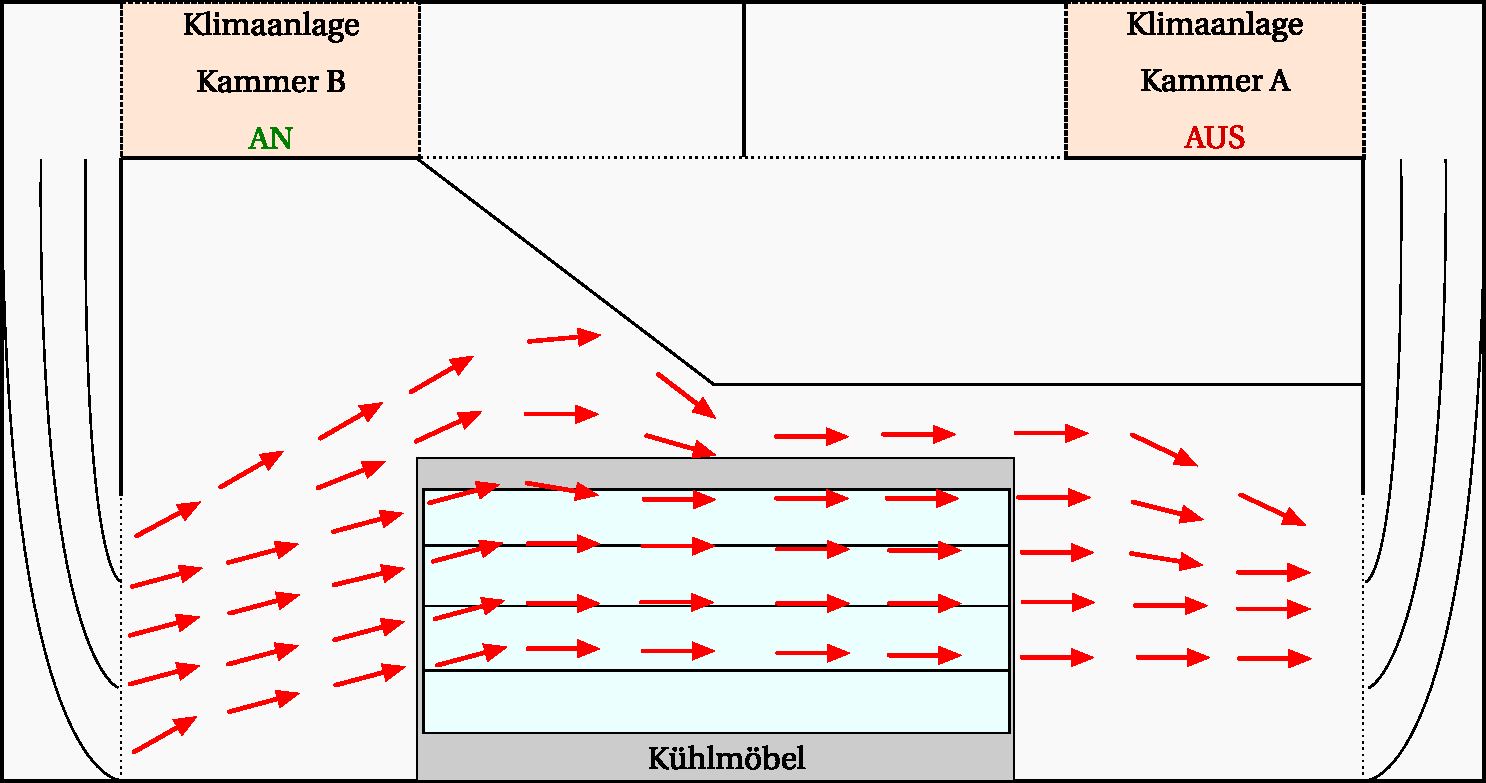
\includegraphics[scale=.6]{Pictures/ClimateChamber_flow30pctCC.pdf}
\caption{Luftströmung in der Klimakammer ohne Deckenöffnung.}
\label{fig:Klimakammer_geschlosseneDecke}
\end{figure}





\clearpage









\section{Kältemittelöle}
\label{sec:EinflussÖl}

In diesem Abschnitt werden die Untersuchungen des Betriebs mit den Kältemittelölen 3MAF und HATCOL~4467 beschrieben und die Untersuchungsergebnisse miteinander verglichen.
Simulationen belegen einen nicht zu vernachlässigenden Anteil im Öl gelösten Kältemittels, was zu einer Minderung der Verdampferleistung führt  \cite{Universitatpolitecnicadevalencia.2017}. Diese führen zu dem Schluss, dass sich ein hoher Anteil des Öles in den Wärmeübertragern befinden muss. Es wird die Annahme gemacht, dass der Ölrücktransport nicht einwandfrei sichergestellt werden kann und dass sich demnach, konservativ abgeschätzt, \unit{20}{\%} des Öles in den Wärmeübertragern befinden. Damit berechnet sich die Menge des im Öl gelösten Kältemittels wie in Tabelle~\ref{tab:LöslichkeitHC3M} dargestellt.
Die berechneten Werte beziehen sich exemplarisch auf einen Kältekreis und basieren auf den Versuchsdaten der Untersuchung von 3MAF.
Mittels der Gleichungen~\ref{eq:1}, \ref{eq:3} und \ref{eq:2} werden die Viskosität, die Dichte und die Löslichkeit des Kältemittels im jeweiligen Öl berechnet. Es ist zu erkennen, dass Propan in 3MAF eine höhere Löslichkeit besitzt als in HATCOL~4467 und dieses folglich mehr Kältemittel aufnehmen kann. In den Wärmeübertragern ist die berechnete Löslichkeit höher als im Verdichter. \newline
In Tabelle~\ref{tab:VergleichKMOele} sind die berechneten Daten der jeweiligen Untersuchungen mit den Ölen 3MAF und HATCOL~4467 aufgeführt. Dabei beziehen sich die Daten im ersten und letzten Abschnitt der Tabelle auf das ganze System und die Daten in den mittleren Abschnitten auf die jeweiligen Kältekreise des Kühlmöbels.
Der Vergleich der Daten beider Untersuchungen zeigt eine um etwa \unit{100}{\watt} höhere elektrische Leistungsaufnahme beim Betrieb mit HATCOL~4467, sowie eine um etwa \unit{60}{\watt} höhere Verdampfungsleistung. Die Kondensationsleistung ist um etwa \unit{300}{\watt} höher. Der EER verzeichnet jedoch eine Reduktion um circa \unit{3}{\%}. Die Verdampfungstemperaturen sowie die Überhitzungen in allen drei Kältekreisen sinken tendenziell. Die Änderung ist sehr gering und bewegt sich im Rahmen der Messungenauigkeit. \newline
Auffällig ist ein Anstieg der Kondensationstemperatur um bis zu \unit{3}{\kelvin}. Diese erreicht in Test~35 nicht die eingestellten \unit{35}{\celsius}. Ein geringes Absinken des Druckabfalls um bis zu \unit{0.05}{\bbar} über den Verdampfer ist zu beobachten. Der Kältemittelmassenstrom sinkt in allen Kreisen sehr gering. In Kreis~1 ist die Reduktion des Massenstroms am deutlichsten. Die Dampfanteile vor den Expansionsventilen sind beim Betrieb mit HATCOL~4467 in allen Kreisen geringer als beim Betrieb mit 3MAF. Dieser Effekt wird in Kreis~1 am deutlichsten. 
Luft- und Produkttemperaturseitig ist keine eindeutige Veränderung zu erkennen. 
Nur die Einlasstemperatur der Luft ist beim Betrieb mit HATCOL~4467 \unit{1}{\kelvin} höher als beim Betrieb mit 3MAF und damit der größte abweichende Wert. \newline
Zuletzt wird mithilfe eines Spülsystems für Kälteanlagen geprüft ob sich zurückgebliebenes Öl in den Kältekreisen befindet. Dieses befördert flüssiges Kältemittel durch das System und sammelt mithilfe eines Ölabscheider eventuell im System verbliebenes Öl.


\clearpage

\begin{table}[h!]
\centering
\caption{Löslichkeitsverhalten von HATCOL~4467 und 3MAF.}
\label{tab:LöslichkeitHC3M}
\begin{tabular}{|cccc|}
\hline
                                           & 10\% Öl im Verdampfer      & 80\% Öl im Verdichter     & 10\% Öl im Kondensator \\ \hline
\multicolumn{1}{|l}{}                      & \multicolumn{3}{c|}{HATCOL~4467}                                                  \\ \hline
\multicolumn{1}{|c|}{Viskosität {[}cSt{]}} & \multicolumn{1}{c|}{3.29}  & \multicolumn{1}{c|}{38.66} & 0.89                    \\
\multicolumn{1}{|c|}{Dichte {[}g/cm³{]}}   & \multicolumn{1}{c|}{0.79}  & \multicolumn{1}{c|}{0.94}  & 0.73                    \\
\multicolumn{1}{|c|}{Löslichkeit {[}\%{]}} & \multicolumn{1}{c|}{35.4}  & \multicolumn{1}{c|}{5.0}   & 37.1                    \\
\multicolumn{1}{|c|}{KM in Öl {[}g{]}}     & \multicolumn{1}{c|}{13.09} & \multicolumn{1}{c|}{17.55} & 12.79                   \\
\multicolumn{1}{|c|}{KM in Öl {[}\%{]}}    & \multicolumn{1}{c|}{8.7}     & \multicolumn{1}{c|}{11.7}    & 8.5                       \\ \hline
\multicolumn{1}{|l}{}                      & \multicolumn{3}{c|}{3MAF}                                                         \\ \hline
\multicolumn{1}{|c|}{Viskosität {[}cSt{]}} & \multicolumn{1}{c|}{1.95}  & \multicolumn{1}{c|}{17.73} & 0.87                    \\
\multicolumn{1}{|c|}{Dichte {[}g/cm³{]}}   & \multicolumn{1}{c|}{0.75}  & \multicolumn{1}{c|}{0.93}  & 0.70                    \\
\multicolumn{1}{|c|}{Löslichkeit {[}\%{]}} & \multicolumn{1}{c|}{41.0}  & \multicolumn{1}{c|}{5.2}   & 41.6                    \\
\multicolumn{1}{|c|}{KM in Öl {[}g{]}}     & \multicolumn{1}{c|}{14.53} & \multicolumn{1}{c|}{18.07} & 13.80                   \\
\multicolumn{1}{|c|}{KM in Öl {[}\%{]}}    & \multicolumn{1}{c|}{9.7}    & \multicolumn{1}{c|}{12.0}    & 9.2                       \\ \hline
\multicolumn{1}{|c|}{Differenz {[}g{]}}    & \multicolumn{1}{c|}{1.45}  & \multicolumn{1}{c|}{0.52}  & 1.01                    \\ \hline
\end{tabular}
\end{table}














\section{Abtauintervalle}
\label{sec:Abtauintervalle}

In diesem Abschnitt werden die Untersuchungen des Betriebs mit einem \unit{4}{\hour} Abtauintervall und mit bedarfsgerechter Abtauung beschrieben und deren Ergebnisse miteinander verglichen. 
Es ist auffällig, dass das Intervall bei bedarfsgerechter Abtauung genau \unit{3}{\hour} lang ist. Dies lässt vermuten, dass die Regelung der Abtauung diese nicht nach Bedarf sondern nach dem eingestellten Intervall von \unit{3}{\hour} einleitet. Daher ist die genaue Ursache für die Abtauung zu prüfen. \newline
Tabelle~\ref{tab:Vergleich4h3h} zeigt die Ergebnisse der beiden Untersuchungen.
Während die elektrische Leistungsaufnahme in etwa gleich groß ist, vergrößern sich bei bedarfsgerechter Abtauung die übertragenen Wärmeströme an den Wärmeübertragern deutlich um circa \unit{350}{\watt}. Dies verursacht eine Erhöhung des EER von \unit{2.14}{} auf \unit{2.26}{}.
Es ist ein Anstieg der Verdampfungstemperaturen in allen drei Kältekreisen um circa \unit{2}{\kelvin} erkennbar. Die Kondensationstemperaturen sind unverändert. Der Massenstrom des Kältemittels steigt um etwa \unit{0.7}{\gram\per\second}. Der Druckabfall über den Verdampfer steigt um etwa \unit{0.05}{\bbar}. Der Dampfanteil des Kältemittels am Kondensatoraustritt steigt um \unit{3}{\%} bis \unit{5}{\%}. Die Auslasstemperatur der Luft steigt um fast \unit{1}{\kelvin} während die Einlasstemperatur der Luft und die Produkttemperaturen unverändert bleiben. \newline
Es ist zu untersuchen, warum eine Verkürzung des Abtauintervalls einen Effizienzgewinn verursacht.

 











\clearpage



\section{Verdichter}
\label{sec:Verdichter}


In diesem Abschnitt werden die Untersuchungsergebnisse des Betriebs mit zwei Ausführungen des in Abschnitt~\ref{sec:Das Kühlregal} vorgestellten Verdichtermodells verglichen. 
Ein Austausch der Verdichter umfasst die Entsorgung der vorherigen Kältemittelfüllung, den Aus- und Einbau der Verdichter sowie eine komplette Inbetriebnahme, inklusive Druckfestigkeits- und Dichtheitsprüfung. Nach erneuter Inbetriebnahme wird das Kühlmöbel bis zum Erreichen einer konstanten Produkttemperatur betrieben. Anschließend beginnt der beobachtete Messzeitraum von \unit{24}{\hour}. \newline
Tabelle~\ref{tab:Verdichterdatenblatt} zeigt die Herstellerdaten beider Verdichtervarianten bei einer Kondensationstemperatur von \unit{35}{\celsius}, einer Verdampfungstemperatur von \unit{-10}{\celsius}, einer Überhitzung von \unit{10}{\kelvin} und einer Unterkühlung von \unit{0}{\kelvin} für einen Verdichter \cite{EmersonClimateTechnologies.},\cite{EmersonClimateTechnologies.2018}. Die Hybridausführung stellt einen um \unit{0.04}{\gram\per\second} höheren Kältemittelmassenstrom bei gleichzeitig um \unit{30}{\watt} geringerer elektrischer Leistungsaufnahme und \unit{10}{\watt} niedrigerer Kälteleistung gegenüber der Standardausführung zur Verfügung.  \newline
Tabelle~\ref{tab:VergleichVerdichter} sind die erfassten und berechneten Messwerte der Untersuchungen zu entnehmen. Diese zeigen eine signifikante Erhöhung der elektrischen als auch der thermischen Leistungen um etwa \unit{400}{\watt} beim Wechsel der Hybrid- zur Standardausführung des Verdichters. Der EER erfährt nur eine geringe Erhöhung um \unit{0.02}{}. Es ist zudem eine Reduzierung des Kältemittelmassenstroms \unit{0.3}{\gram\per\second} bis \unit{0.5}{\gram\per\second} zu erkennen und eine Reduzierung des Dampfanteils am Kondensatoraustritt um \unit{5}{\%} bis \unit{14}{\%}. In Kreis~2 ist dies besonders gut zu erkennen. Der Druckabfall in den Kreisen~2 und 3 erfährt eine Reduktion während der Druckabfall sehr gering ansteigt. Die kältekreis- und luftseitig erfassten Temperaturen sowie Temperaturdifferenzen unterscheiden sich nicht signifikant. Die Änderungen liegen im Bereich der Messungenauigkeit. Der Vergleich mit den Herstellerdaten zeigt, dass sich das System entgegengesetzt der Voraussagen verhält. Statt einem höheren Massenstrom und geringerer elektrischer Leistungsaufnahme stellt sich ein niedrigerer Massenstrom bei erhöhter elektrischer Leistungsaufnahme ein. Es ist zu untersuchen warum das System sich anders verhält als durch die Herstellerdaten zu erwarten.\newline
Die log-p-h-Diagramme~\ref{fig:logph51} und \ref{fig:logph54} zeigen das Zwei-Phasen-Gebiet von R290 im Anwendungsbereich. Auf der x-Achse ist die Enthalpie in $\frac{kJ}{kg}$ und auf der y-Achse logarithmisch der Druck in $bar$ aufgetragen. Der Vergleich zeigt die Erhöhung der Kondensations- sowie der Verdampfungsenthalpie nach Wechsel zur Standardausführung exemplarisch an Kreis 2. Die Werte werden jeweils \unit{10}{\%} vor Ende des letzten Zyklus erfasst. Es ist zu untersuchen, was die Erhöhung der Enthalpiedifferenz verursacht und warum eine Leistungserhöhung erzielt wird.

\begin{table}[h!]
\centering
\caption{Herstellerdaten.}
\label{tab:Verdichterdatenblatt}
\begin{tabular}{|ccc|}
\hline
                                            & ZB09KAU-TFD (Hyb)         & ZB09KAU-TFD \\ \hline
\multicolumn{1}{|c|}{Kälteleistung {[}W{]}} & \multicolumn{1}{c|}{2280} & 2290        \\
\multicolumn{1}{|c|}{el. Leistung {[}W{]}}  & \multicolumn{1}{c|}{830}  & 800         \\
\multicolumn{1}{|c|}{Massenstrom {[}g/s{]}} & \multicolumn{1}{c|}{7.96} & 8.00        \\ \hline
\end{tabular}
\end{table}


\begin{figure}[h!]
\centering
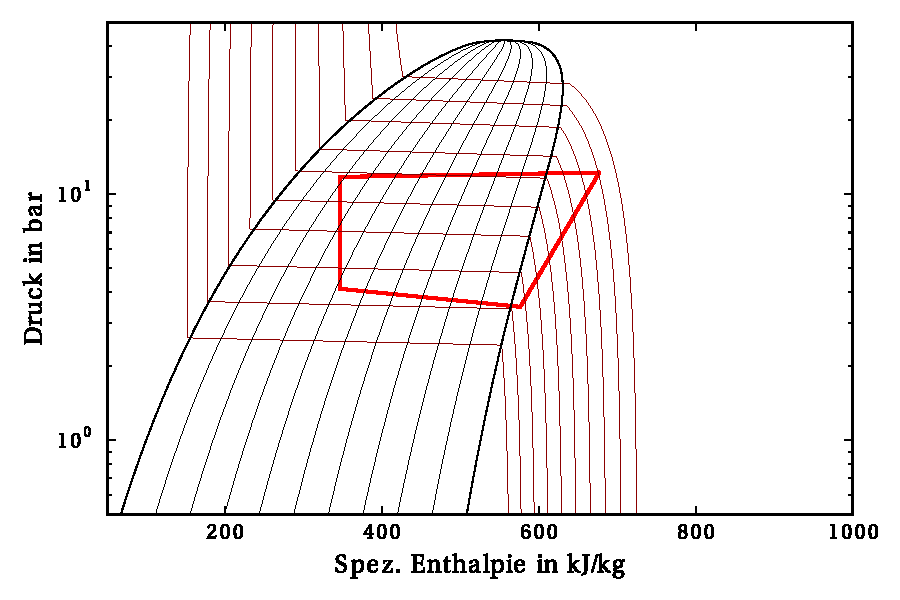
\includegraphics[scale=0.8]{Pictures/51/log_ph_lastCycle10perc_C21.pdf}
\caption{logp-h-Diagramm (K2) beim Betrieb mit Verdichtermodell ZB09KAU-TFD (Hybrid) \unit{10}{\%} vor Ende des Zyklus.}
\label{fig:logph51}
\end{figure}

\begin{figure}[h!]
\centering
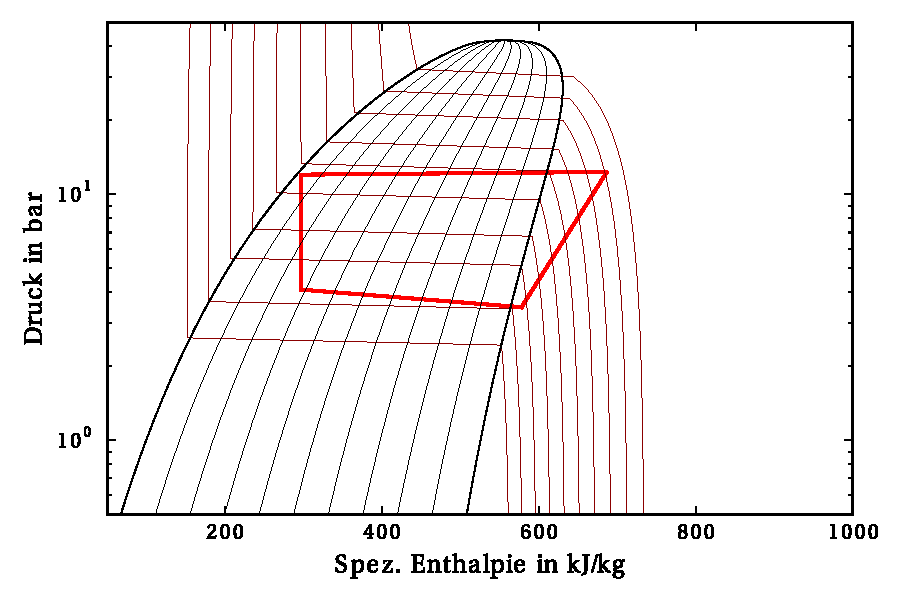
\includegraphics[scale=0.8]{Pictures/54/log_ph_lastCycle10perc_C21.pdf}
\caption{logp-h-Diagramm (K2) beim Betrieb mit Verdichtermodell ZB09KAU-TFD \unit{10}{\%} vor Ende des Zyklus.}
\label{fig:logph54}
\end{figure}






\clearpage





\section{Änderung der Verdampferschaltung}
\label{sec:Änderung der Verdampferschaltung}

In diesem Unterkapitel wird der Wechsel der Verdampfer und deren Verschaltungen sowie die daran durchgeführten Untersuchungen beschrieben. Abbildung~\ref{fig:Verschaltungsarten} zeigt die untersuchten Verdampfer und ihre Verschaltungsarten. Der bei AHT-Kühlmöbeln standardmäßig verbaute Verdampfer ist zweireihig und besitzt zwecks Kostenreduzierung nur die Kupferrohre, die tatsächlich mit Kältemittel beaufschlagt werden. In den Lamellen sind dennoch die Lochungen samt deren Grate für weitere Rohre vorhanden, sodass die reduzierte Rohranzahl nicht die Luftströmung innerhalb des Verdampfers beeinflusst. Im Anschluss soll ein vierreihiger Verdampfer mit versetzten Rohren untersucht werden. Dieser besitzt eine Verschaltung wie sie in Kühlmöbeln von LIDL zu finden ist und mehr Kupferrohre als für die Kältekreise benötigt werden. Der Verdampfer verspricht einen höheren kA-Wert und damit nach Gleichung~\ref{eq:4} einen höheren übertragbaren Wärmestrom. Mithilfe des in Abschnitt~\ref{sec:Simulationsmodell} präsentierten Simulationsmodells werden die Verschaltungen V1 und V2 zur Validierung des Modells bei \unit{0}{\%} r.F.  miteinander verglichen. Zuletzt werden die Untersuchungsergebnisse beider Verschaltungen unter den Normbedingungen bei \unit{60}{\%} r. F miteinander verglichen, um die Verschaltung unter Normbedingungen bewerten zu können.

\begin{figure}[h!tb]
\centering
	\subfigure[AHT-Verdampfer]{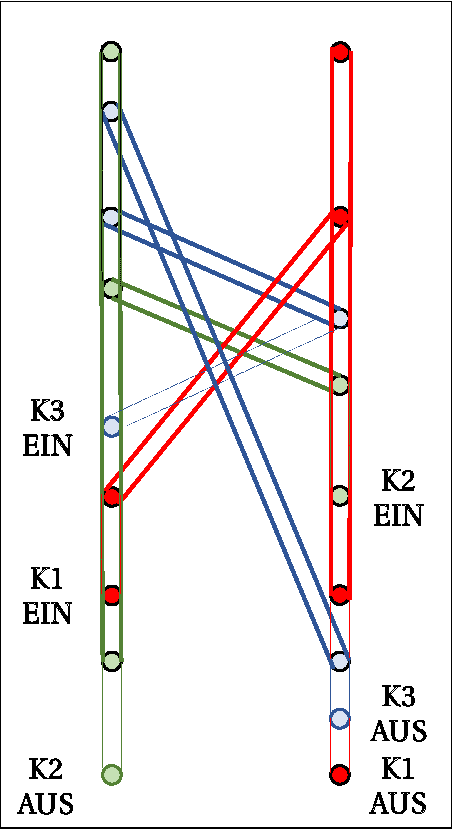
\includegraphics[scale=.65]{Pictures/AHTEV.pdf}}
	\subfigure[LIDL-Verdampfer V1]{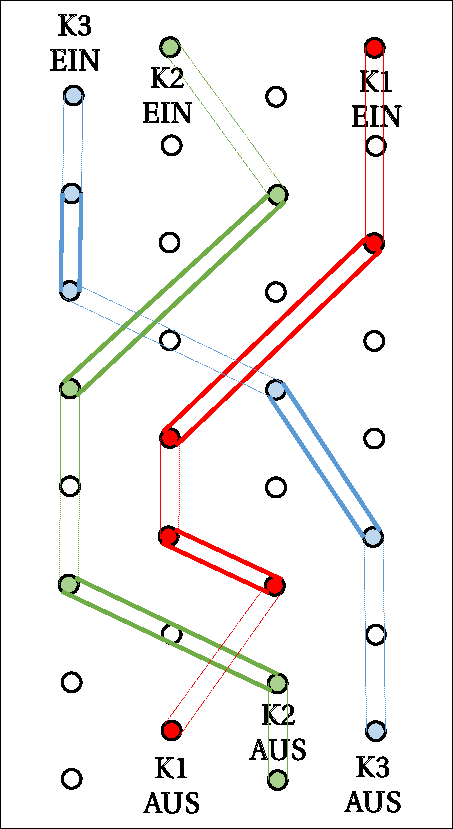
\includegraphics[scale=.65]{Pictures/LIDLV1.pdf}}
	\subfigure[LIDL-Verdampfer V2]{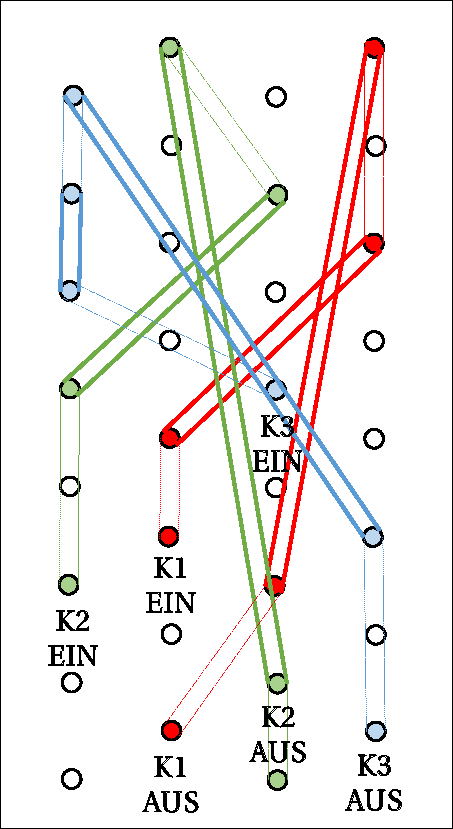
\includegraphics[scale=.65]{Pictures/LIDLV2.pdf}}
\caption{Die untersuchten Verdampfer und Verschaltungsarten.}
\label{fig:Verschaltungsarten}
\end{figure}




\subsection{Vergleich zwischen Verdampfern}
\label{subsec:Vergleich zwischen Verdampfern}

In diesem Abschnitt wird der Umbau des Kühlmöbels beschrieben und die Ergebnisse der Untersuchungen des zweireihigen AHT-Verdampfers und des vierreihigen LIDL-Verdampfers mit versetzten Reihen beschrieben und verglichen. Der neue Verdampfer besitzt die gleichen Abmessungen wie der vorige. Rohrdurchmesser und Rohrdicke sind identisch. Der Einbau eines neuen Verdampfers im Kühlmöbel erfordert zunächst eine komplette Demontage des Innenraums. Das Kältemittel der Anlage wird entsorgt. Die M-Pakete werden entfernt und zwischengelagert. Daraufhin werden die Regalbretter, die Verkleidungen des Bodens, der Rückwand sowie der Decke und die Seitenwände demontiert. Die Abdeckungen des Verdampfers und die Lüfter müssen entfernt werden. Bevor die Lötverbindungen des Verdampfers getrennt werden können müssen noch alle Temperatursensoren entfernt werden. Anschließend erfolgt ein Austausch des Verdampfers durch die LIDL-Ausführung und eine Montage des kompletten Kühlmöbels in umgekehrter Reihenfolge der zuvor beschriebenen Schritte. Danach wird die Anlage erneut mit \unit{150}{\gram} Propan pro Kreis gefüllt. Vor Inbetriebnahme des Kühlmöbels wird eine Dichtheits- und eine Druckfestigkeitsprüfung an den drei Kältekreisen durchgeführt. Unter gleichen Bedingungen wie zuvor wird erneut eine Untersuchung durchgeführt. \newline 
In Tabelle~\ref{tab:Vergleichaltneu} sind die Ergebnisse der Untersuchungen des Betriebs mit dem alten AHT-Verdampfer sowie dem neuen LIDL-Verdampfer dargestellt.
Der Vergleich zeigt eine Reduktion der thermischen Leistungen um etwa \unit{1000}{\watt} bei gleichbleibender elektrischer Leistungsaufnahme. Dies resultiert in einer Reduktion des EER um \unit{16.2}{\%} von \unit{2.28}{} auf \unit{1.91}{}. In den Kältekreisen ist ein Anstieg der Verdampfungstemperaturen um \unit{3}{\kelvin} bis \unit{5}{\kelvin} zu erkennen. Die Kondensationstemperaturen bleiben etwa konstant. Lediglich in Kreis~3 weicht diese um fast \unit{1}{\kelvin} nach unten ab. Die Überhitzung ist während des Betriebs mit dem LIDL-Verdampfer um \unit{3}{\kelvin} bis \unit{4}{\kelvin} größer. Auffällig ist, dass mit dem Einbau des neuen Verdampfers die vom Expansionsventil erfasste Überhitzung stets um etwa \unit{2}{\kelvin} von der messtechnisch erfassten Überhitzung nach oben abweicht. Der Dampfanteil ist um bis zu \unit{28}{\%} größer und liegt bei \unit{35}{\%} und \unit{34}{\%} in den Kreisen 1 und 2 und bei \unit{43}{\%} in Kreis 3. Der Massenstrom des Kältemittels ist in allen Kreisen etwa \unit{1}{\gram} bis \unit{1.5}{\gram} größer. Der Druckabfall über den Verdampfer ist \unit{0.1}{\bbar} größer. \newline
Bei der Betrachtung der Produkt- und Lufttemperaturen ist eine deutliche Erhöhung dieser Messwerte auffällig. Die Durchschnittstemperatur der Produkte ist um fast \unit{2}{\kelvin} höher. Die minimale Produkttemperatur steigt stark von circa \unit{1}{\celsius} auf fast \unit{4}{\celsius} an während die maximale Produkttemperatur unverändert ist. Die Ein- und Auslasstemperaturen der Luft sind ebenso um \unit{2}{\kelvin} höher. \newline
Es ist zu untersuchen warum der Verdampferaustausch eine derartige Verschlechterung hinsichtlich der erzielten Leistungen und Temperaturen mit sich führt.


\clearpage

\subsection{Modellgestützter Vergleich der Verschaltungen V1 und V2}
\label{subsec:Modellgestützter Vergleich der Verschaltungen V1 und V2}

In diesem Abschnitt wird die Modellbildung sowie der Verdampferumbau erläutert und die Simulationsergebnisse mit den Versuchsdaten verglichen.
Zunächst wird, wie in Abschnitt~\ref{sec:Simulationsmodell} beschrieben, ein Modell mithilfe des Programms EES entwickelt. Wegen der angewandten $\epsilon$-$NTU$-Methode ist das Modell nur gültig für trockene Luft \cite{Bergman.2011}. Basierend auf dieser Annahme ist es nötig, die Berechnung ganzheitlich für trockene Luft durchzuführen sowie das Modell mit Versuchsdaten von Untersuchungen bei \unit{0}{\%} relativer Feuchtigkeit zu validieren. In der Klimakammer sind bei dieser Einstellung lediglich relative Feuchtigkeiten zwischen \unit{5}{\%} und \unit{25}{\%} erzielbar. Am Lufteinlass des Verdampfers beträgt die relative Feuchtigkeit etwa \unit{40}{\%}, weswegen mit einer äquivalenten Temperatur gerechnet werden muss. Bei konstanter Enthalpie entspricht die Ist-Temperatur von \unit{4.42}{\celsius} bei \unit{40}{\%} r.F. einer äquivalenten Temperatur von \unit{9.75}{\celsius} bei \unit{0}{\%} r.F.. \newline
Für die Berechnung der Wärmeleitwiderstände, mittels der Gleichungen~\ref{eq:28} bis \ref{eq:31}, ist es notwendig die Wärmeübergangs- und Wärmeleitkoeffizienten zu bestimmen. Eine Berechnung dieser Werte mittels geeigneter Modelle liefert fehlerhafte Werte infolgederer das Modell instabil ist. Um den Rechenaufwand sowie Fehlerquellen gering zu halten werden die in Tabelle~\ref{tab:Werte der Wärmeübergangs- und Wärmeleitzahlen} dargestellten Annahmen getroffen \cite{Bergman.2011},\cite{Recknagel.2005},\cite{DINDeutschesInstitutfurNormunge.V..2017d}. Dabei werden die Wärmeübergangskoeffizienten der Luft $\alpha_L$, des Kältemittels $\alpha_{KM}$ und des überhitzten Kältemittels $\alpha_{KM,SH}$ so gewählt, dass das errechnete Temperaturprofil des Kältemittels dem erfassten Temperaturprofil, auf Basis der Messwerte von Untersuchung~61, entspricht. 
Für die Berechnung der Rohrstrecken, welche mit zweiphasigem Kältemittel beaufschlagt werden, werden Gleichung~\ref{eq:33} und der Wärmeübergangskoeffizient $\alpha_{KM}$ verwendet. Aus dem erfassten Temperaturprofil ist ersichtlich, dass nur die letzte Rohrstrecke überhitzt ist. Für diese werden Gleichung~\ref{eq:34} und der Wärmeübergangskoeffizient $\alpha_{KM,SH}$ verwendet. \newline
Das Modell wird exemplarisch für einen Kältekreis im Verdampfer erstellt. Damit die Ergebnisse vergleichbar mit denen der Untersuchungen sind wird mit einem Drittel des Luftmassenstroms gerechnet. 

\begin{table}[h!]
\centering
\caption{Werte der Wärmeübergangs- und Wärmeleitkoeffizienten.}
\label{tab:Werte der Wärmeübergangs- und Wärmeleitzahlen}
\renewcommand{\arraystretch}{1.2}
\begin{tabular}{|l|l|l|}

\hline
Parameter        & Wert  & Einheit           \\ \hline
$\alpha_{L}$     & 292   & $\frac{W}{m^2 K}$ \\
$\alpha_{KM}$    & 50000 & $\frac{W}{m^2 K}$ \\
$\alpha_{KM,SH}$ & 29    & $\frac{W}{m^2 K}$ \\
$\lambda_{Cu}$   & 380   & $\frac{W}{m K}$   \\
$\lambda_{Al}$   & 220   & $\frac{W}{m K}$   \\ \hline
\end{tabular}
\end{table}

Die Simulation liefert Ergebnisse für die in Abbildung~\ref{fig:Vergleich der Verdampferschaltungen} dargestellten Verschaltungen. Ein Vergleich der Simulationsergebnisse mit den Untersuchungsergebnissen von Verschaltung~V2 bei \unit{0}{\%} relativer Luftfeuchtigkeit ermöglicht die Validierung des Modells. Dafür muss zunächst die Verschaltung des Verdampfers verändert werden. Eine komplette Demontage des Kühlmöbels wie zuvor beim Tausch des Verdampfers ist dabei nicht nötig. Es genügt eine Demontage der rechten Seite des Kühlmöbels und beider Seitentrennwände um an den Seiten des Verdampfers arbeiten zu können. Zunächst wird das Kältemittel entsorgt. Die Einspritzleitung wird an die Stelle des zuvorigen Endes des vierten Verdampferrohres gesetzt und zwischen dem ersten und fünften Verdampferrohr eine neue Verbindung hergestellt. Im Anschluss werden die Temperaturfühler entsprechend neu positioniert. Bevor eine erneute Untersuchung durchgeführt werden kann wird eine Dichtheits- und eine Druckfestigkeitsprüfung an den drei Kältekreisen durchgeführt. Beim bisherigen Sollwert von \unit{8}{\kelvin} öffnet das Ventil komplett, sodass eine Regelung der Überhitzung nicht möglich ist. Deshalb wird für die weiteren Untersuchungen am neuen Verdampfer der Sollwert der Überhitzung an den drei Expansionsventilen auf \unit{13}{\kelvin} geändert. \newline 
Im Folgenden werden die Ergebnisse der Simulation mit denen der Untersuchungen bei \unit{0}{\%} relativer Feuchtigkeit verglichen. Tabelle~\ref{tab:VergleichSimuUntersuchung} zeigt die Messwerte der Untersuchungen von Verschaltung~ V1 und V2 und die Simulationsergebnisse beider Verschaltungen. Dabei beziehen sich die Messwerte exemplarisch auf Kältekreis~1. 
Im Vergleich der Untersuchung von Verschaltung~V1 mit deren Simulationsergebnissen fällt auf, dass der errechnete Druckabfall um \unit{0.2}{\bbar} geringer ist als der tatsächlich erzielte. Die erzielte Verdampfungstemperatur ist dementsprechend höher.
Kältemittelmassenstrom und Einlasstemperatur der Luft sind konstant, da dies die Eingangsgrößen des Modells sind. Die errechnete Auslasstemperatur ist um etwa \unit{0.5}{\kelvin} höher als die tatsächliche. Die errechnete Kälteleistung weicht mit etwa \unit{30}{\watt} sehr gering von der tatsächlichen ab.  \newline Werden die Simulationsergebnisse beider Verschaltungen miteinander verglichen, so ist ein geringer Anstieg des Druckabfalls um etwa \unit{0.03}{\bbar} zu erkennen. Dies hat eine Reduzierung der Verdampfungstemperatur um \unit{0.25}{\kelvin} zur Folge. Die Kälteeistung ist um \unit{19}{\watt} höher. Dies spiegelt sich in einer sehr geringen Absenkung der Luftauslasstemperatur um \unit{0.15}{\kelvin} wider. Diese Änderungen sind zwar gering, belegen aber tendenziell die These, dass eine Änderung der Verschaltung eine Erhöhung der Kälteleistung erzielt. \newline
Zuletzt wird der Effekt der Verschaltungsänderung im Modell mit dem in der Untersuchung erzieltem Effekt verglichen. Dies ermöglicht eine Beurteilung der Modelltauglichkeit. Der tatsächliche Druckabfall erfährt eine Erhöhung um etwa \unit{0.06}{\bbar}. Das ist doppelt so viel wie die berechnete Änderung. Dies resultiert in einer stärkeren Absenkung der Verdampfungstemperatur um etwa \unit{1.4}{\kelvin}. Während die Einlasstemperatur der Luft bei Verschaltung~V2 um etwa \unit{0.5}{\kelvin} höher ist, weicht die Auslasstemperatur der Luft vernachlässigbar gering nach unten ab. Mittels des Modells wird eine Erhöhung der Temperaturdifferenzen zwischen Ein- und Austritt um \unit{0.15}{\kelvin} vorausgesagt. Die Untersuchungen zeigen eine Erhöhung der Temperaturdifferenz um \unit{0.71}{\kelvin}. Die Messwerte der Untersuchungen belegen damit die Tendenz des Modells. Es ist zu untersuchen, warum der errechnete Druckabfall nur etwa halb so groß wie der tatsächliche ist. \newline




\clearpage


\begin{table}[h]
\centering
\caption{Vergleich der Simulation mit den Untersuchungen.}
\label{tab:VergleichSimuUntersuchung}
\begin{tabular}{|ccccc|}
\hline
                                                      & Untersuchung V1             & Modell V1                   & Modell V2                   & Untersuchung V2 \\ \hline
\multicolumn{1}{|c|}{Druckabfall {[}Pa{]}}            & \multicolumn{1}{c|}{47192}  & \multicolumn{1}{c|}{27175}  & \multicolumn{1}{c|}{29889}  & 52996           \\
\multicolumn{1}{|c|}{Kälteleistung {[}W{]}}           & \multicolumn{1}{c|}{1791}   & \multicolumn{1}{c|}{1812}   & \multicolumn{1}{c|}{1831}   & 1827            \\
\multicolumn{1}{|c|}{Verdampfungstemperatur {[}°C{]}} & \multicolumn{1}{c|}{-14.15} & \multicolumn{1}{c|}{-12.23} & \multicolumn{1}{c|}{-12.48} & -15.59          \\
\multicolumn{1}{|c|}{Massenstrom KM {[}g/s{]}}        & \multicolumn{1}{c|}{6.11}   & \multicolumn{1}{c|}{6.11}   & \multicolumn{1}{c|}{6.11}   & 5.72            \\
\multicolumn{1}{|c|}{Einlasstemperatur Luft {[}°C{]}} & \multicolumn{1}{c|}{4.42}   & \multicolumn{1}{c|}{4.42}   & \multicolumn{1}{c|}{4.42}   & 5.07            \\
\multicolumn{1}{|c|}{Auslasstemperatur Luft {[}°C{]}} & \multicolumn{1}{c|}{-5.38}  & \multicolumn{1}{c|}{-4.8}   & \multicolumn{1}{c|}{-4.95}  & -5.44           \\
\hline
\end{tabular}
\end{table}


Die Abbildungen~\ref{fig:SimTempV1} und \ref{fig:SimTempV2} zeigen die Temperaturprofile der Luft und des Kältemittels über jeden berechneten Verdampferdurchgang in Verschaltung V1 bzw. V2. Auf der x-Achse sind die Verdampferpässe auf die Höhe des Verdampfers bezogen aufgetragen, auf der y-Achse die Temperatur in °$C$. Der Effekt der Verschaltungsänderung auf das Temperaturprofil des Kältemittels ist gut zu erkennen. Statt zunächst Abzusinken steigt die Verdampfungstemperatur an. Dadurch wird am Luftaustritt des Verdampfers eine tiefere Temperatur erzielt. Die erzielte Änderung ist jedoch grafisch kaum sichtbar. Im vierten Verdampferdurchgang beginnt das Kältemittel zu überhitzen. Der Anstieg ist zunächst steiler als im fünften und sechsten Verdampferpass. In Verschaltung V2 überhitzt das Kältemittel auf eine höhere Temperatur als in V1. Es ist zu untersuchen, warum das Modell eine stärkere Überhitzung des Kältemittels vorraussagt. \newline
Im Folgenden werden die Messwerte und Berechnungsergebnisse der Untersuchungen mit den Verschaltungen V1 und V2 bei einem Sollwert von \unit{0}{\%} r.F. in der Kammer miteinander verglichen. In Tabelle~\ref{tab:VergleichV1V2_0rF} werden diese dargestellt. Während die elektrische Leistung nach Änderung der Verschaltung eine geringe Reduktion um \unit{16}{\watt} verzeichnet, erfährt die thermische Leistung des Verdampfers eine Erhöhung um circa \unit{140}{\watt} und die des Kondensators um \unit{50}{\watt}. Dies resultiert in einer Erhöhung des EERs um \unit{4}{\%} von \unit{1.99}{} auf \unit{2.07}{}.
Die Verdampfungstemperaturen in allen Kältekreisen erfahren eine Absenkung um circa \unit{1.5}{\kelvin}. Gegenüber den Untersuchungen bei \unit{60}{\%} r.F. sind diese sehr niedrig. Die Kondensationstemperaturen bleiben unbeeinflusst. Die Änderung der gemessenen Überhitzungen ist vernachlässigbar gering. Nur in Kreis 3 ist diese um etwa \unit{1}{\kelvin} höher. Auffällig ist, dass in der neuen Verschaltung der Dampfanteil in den drei Kreisen \unit{0}{\%} beträgt und damit eine Unterkühlung von etwa \unit{3}{\kelvin} bis \unit{4}{\kelvin} erzielt wird. Die Massenströme erfahren eine Reduktion um etwa \unit{0.5}{\gram\per\second}. Der Druckabfall verzeichnet in Kreis~1 einen Anstieg um \unit{0.05}{\bbar} und in Kreis~2 einen sehr geringen Anstieg um \unit{0.01}{\bbar}. In Kreis~3 verzeichnet der Druckabfall hingegen eine Reduktion um \unit{0.01}{\bbar}. Die Produkt- und Lufttemperaturen lassen erkennen, dass diese wie die Verdampfungstemperatur sehr niedrig sind. Gegenüber Verschaltung~V1 ist bei V2 keine Änderung ersichtlich. Nur die maximale Produkttemperatur ist um \unit{1}{\kelvin} höher. Damit einher geht eine Erhöhung der Durchschnittstemperatur um etwa \unit{0.6}{\kelvin}. Es ist zu untersuchen, warum die Temperaturen derart niedrig sind und ob die erfassten Messwerte die Berechnungen des Modells bestätigen.

\begin{figure}[h!]
\centering
\includegraphics[scale=0.8]{Pictures/Temp_V11.pdf}
\caption{Simuliertes Temperaturprofil des Verdampfers für Verschaltung V1.}
\label{fig:SimTempV1}
\end{figure}

\begin{figure}[h!]
\centering
\includegraphics[scale=0.8]{Pictures/Temp_V21.pdf}
\caption{Simuliertes Temperaturprofil des Verdampfers für Verschaltung V2.}
\label{fig:SimTempV2}
\end{figure}
\subsection{Vergleich der Verschaltungen V1 und V2}
\label{subsec:Vergleich der Verschaltungen V1 und V2}

In diesem Abschnitt werden die Untersuchungsergebnisse der Verschaltungen V1 und V2 unter den normalen Prüfbedingungen bei \unit{60}{\%} relativer Luftfeuchtigkeit miteinander verglichen. Der Umbau ist bereits erfolgt. Es ist lediglich eine erneute Untersuchung bei vorherigen Bedingungen erforderlich. Der Sollwert der Überhitzung beträgt \unit{13}{\kelvin}. \newline
Tabelle~\ref{tab:VergleichV1V2_60rF} stellt die Messwerte und Berechnungsergebnisse der Untersuchungen mit den Verschaltungen V1 und V2 bei einem Sollwert von \unit{60}{\%} r.F. in der Kammer dar. Die elektrische Leistung erfährt eine Reduktion um \unit{16}{\watt}, die thermische Leistung des Verdampfers hingegen erfährt einen Anstieg um \unit{140}{\watt} und die des Kondensators um etwa \unit{100}{\watt}. Dies resultiert in einem Anstieg des EERs um \unit{3}{\%} von \unit{2.21}{} auf \unit{2.28}{}.
Die Verdampfungstemperatur in den drei Kältekreisen ist um etwa \unit{1.5}{\kelvin} geringer. Die Kondensationstemperatur sowie die erfasste Überhitzung sind unverändert.
Während in Verschaltung~V1 keine Unterkühlung erzielt wird und die Dampfanteile zwischen \unit{4}{\%} und \unit{19}{\%} liegen, werden diese in der neuen Verschaltung auf \unit{0}{\%} reduziert. Dadurch wird zwar Unterkühlung erzielt, diese ist jedoch mit etwa \unit{0.2}{\kelvin} sehr gering. Der Massenstrom des Kältemittels erfährt eine Reduktion um \unit{0.5}{\gram\per\second}. Der Druckabfall steigt in Kreis~1 um etwa \unit{0.06}{\bbar}, in den Kreisen~2 und 3 um \unit{0.01}{\bbar} bis \unit{0.02}{\bbar} an. Der Vergleich der Produkttemperaturen zeigt eine Reduktion der maximalen Temperatur um \unit{0.5}{\kelvin} und der minimalen Temperatur um \unit{1.5}{\kelvin}. Dies resultiert in einer um \unit{0.5}{\kelvin} geringeren Durchschnittstemperatur.
Während die Einlasstemperatur der Luft nahezu konstant ist verzeichnet die Auslasstemperatur eine Reduktion um etwa \unit{0.8}{\kelvin}.
Es ist zu untersuchen, ob sich das System hinsichtlich dieser Werte ähnlich verhält wie in Untersuchung bei \unit{0}{\%} r.F.. Daraus kann abgeleitet werden ob die Vorhersagen des Modells auch für den Betrieb bei Normbedingungen gültig sind.




%%%%%%%%%%%%%%%%%%%%%%%%%%%%%%%%%%%%%%%%%%%%%%%%%%%%%%


\chapter{Analyse der Messergebnisse}
\label{cha:Analyse der Messergebnisse}

\section{Einstellung von Normbedingungen}
\label{sec:Einstellung von Normbedingungen_1}

In diesem Abschnitt werden die Ergebnisse aus Abschnitt~\ref{sec:EinstellungvonNormbedingungen} erläutert und die daraus abgeleiteten Konsequenzen erklärt. Anhand der Abbildungen~\ref{fig:10pctOC} - \ref{fig:30pctCC} lässt sich erkennen, dass die Geschwindigkeiten beim Betrieb mit fünf Lüftern mit je \unit{10}{\%} ihrer Leistung näher an der geforderten Normgeschwindigkeit liegen als beim Betrieb mit zwei Lüftern bei \unit{30}{\%} Leistung. Hierbei ist ein höherer Turbolenzgrad aufgrund der größeren Schwankung der Messwerte ersichtlich. Ein höherer Turbolenzgrad hat einen höheren Durchmischungsgrad der Raumluft mit der kalten Luft des Luftschleiers zur Folge. 
Werden diese Erkenntnisse den Ergebnissen der Untersuchungen mit einer geschlossenen Decke gegenübergestellt, so ist zu erkennen, dass das Schließen der Decke eine Minderung des Turbolenzgrades zur Folge hat. \
Der beim Vergleich der Abbildungen~\ref{fig:10pctOC_temp} und \ref{fig:30pctOC_temp} ersichtliche höhere Temperaturgradient bei niedrigerer Lüfterleistung ist ebenfalls auf den höheren Turbolenzgrad zurückzuführen. \
Aufgrund der relativ geringen Luftgeschwindigkeit ist die Auftriebskraft sehr einflussreich auf das Strömungsbild. Die warme Luft steigt bei Eintritt in den Raum langsam an die Decke und zieht sich dort entlang bis zur Öffnung in der Decke bzw. bis sie gezwungen ist in den weiter unten liegenden Luftauslass von Kammer A zu strömen.
Letzteres hat, wie aus Abbildung ~\ref{fig:Klimakammer_geschlosseneDecke} ersichtlich eine gleichmäßigere und über die Länge des Kühlmöbels konstante Strömung zur Folge.
Jedoch führt diese vermeintlich bessere Maßnahme zu großen Unregelmäßigkeiten in der Regelung der Durchschnittstemperatur und der relativen Luftfeuchtigkeit der Klimakammer. \newline
Aufgrund dessen und aus Gründen der Vergleichbarkeit mit vorherigen Untersuchungen wurde entschieden, dass die Abdeckung der Öffnung in der Decke wieder entfernt wird. Wegen des geringeren Temperaturgradienten wurde für alle weiteren Untersuchungen der Betrieb mit zwei Lüftern bei je \unit{30}{\%} ihrer Leistung festgelegt.












\section{Kältemittelöle}
\label{sec:Kältemittelöleanalyse}

In diesem Abschnitt wird der Einfluss der Kältemittelöle 3MAF und HATCOL~4467 auf das Systemverhalten analysiert.
Wie in Abschnitt~\ref{sec:EinflussÖl} beschrieben ist auffällig, dass die Sättigungstemperatur des Kältemittels im Kondensator unter der Eintrittstemperatur des Wassers liegt. Dies ist durch einen geringen Druck in der Flüssigkeitsleitung zu erklären. Der Hersteller der Kondensatoren gibt bei vollständiger Kondensation einen maximalen Druckabfall von \unit{0.0117}{\bbar} an \cite{SWEP.2017}. Ein sehr hoher Dampfanteil im Kondensator und in der Flüssigkeitsleitung sowie ein hoher Massenstrom verursachen, nach Gleichung~\ref{eq:14}, einen großen Druckabfall. Durch Absinken des Druckes sinkt die Sättigungstemperatur des Kältemittels und folglich die Differenz zwischen Eingangstemperatur des Wassers und Temperatur des Kältemittels. Dies führt dazu, dass am Kondensator keine Wärme mehr übertragen werden kann und das Kältemittel nicht in der Lage ist weiter zu kondensieren bzw. zu unterkühlen. Der geringere Druckabfall über den Verdampfer ist durch den geringeren Kältemittelmassenstrom zu erklären. Die Reduktion des Kältemittelmassenstroms ist auf eine Reduktion des Öffnungsgrades des Expansionsventiles zurückzuführen. Aufgrund des relativ hohen Dampfanteiles vor dessen Einlass und der verschiedenen Öleigenschaften ist zu erwarten, dass sich das Regelverhalten der Ventile in beiden Untersuchungen leicht voneinander unterscheidet. Dies wird durch die Messergebnisse bestätigt. \newline
Wie Tabelle~\ref{tab:LöslichkeitHC3M} zu entnehmen, ist die Löslichkeit des Kältemittels in HATCOL~4467 in den Wärmeübertragern etwas geringer als die in 3MAF. Das Öl nimmt weniger Kältemittel auf, wodurch mehr Leistung zur Verfügung steht, da mehr Kältemittel sofort verdampfen kann. 3MAF besitzt mit der höheren Kältemittellöslichkeit hingegen bessere Ölrückführungseigenschaften. Der rechnerische Unterschied im Verdichter ist vernachlässigbar gering.
Der Versuch bestätigt die rechnerischen Vorhersagen. Ein Wechsel des Öles zu HATCOL~4467 führt zu einer Vergrößerung der Wärmeübertragerleistungen. Dies hat auch eine überproportionale Erhöhung der elektrischen Leistungsaufnahme zu Folge, was sich negativ auf den EER auswirkt.
Produkt- und lufttemperaturseitig ist nur ein geringer Effekt des Ölwechsels zu beobachten. Dieser liegt im Bereich der Messungenauigkeit und ist als vernachlässigbar zu deuten. Die wärmere Eintrittstemperatur ist wahrscheinlich auf Unregelmäßigkeiten in der Durchmischung mit dem warmen Luftstrom der Klimakammer zurückzuführen. Deswegen ist es schwierig das System anhand der erzielten Produkttemperaturen zu bewerten.
Die Annahme, dass der Öltransport im System nicht optimal ist wird durch das Spülen des Systems widerlegt. Dieses führt zu der Erkenntnis, dass sich bei ausgeschalteter Anlage kein zurückgebliebenes Öl in dieser befindet. Die Ölwurfrate des Verdichters ist der leistungsbeeinflussende Parameter. Ist diese gering, so ist die Reduktion der Nutzkälteleistung durch mitgeführtes Öl in den Wärmeübertragern ebenfalls gering. \newline
Mit alleinigem Hinblick auf die Verdampferleistung ist HATCOL~4467 vorzuziehen.
Da sich dies negativ auf den EER auswirkt und produkttemperaturseitig kein Einfluss zu erkennen ist lohnt sich der Betrieb mit 3MAF.





\clearpage




\section{Abtauintervalle}
\label{sec:AbtauintervalleAnalyse}

In diesem Abschnitt wird der Einfluss der Länge der Abtauintervalle auf das Systemverhalten auf Basis der in Abschnitt~\ref{sec:Abtauintervalle} beschriebenen Untersuchungsergebnisse analysiert. \newline
Zunächst ist zu untersuchen, warum die Abtauung genau nach \unit{3}{\hour} eingeleitet wird. Zu diesem Zweck wird die Abtauregelung der Steuerungssoftware betrachtet. Diese ist schematisch in Abbildung~\ref{fig:bedarfsgerechteAbtauung} dargestellt \cite{EmersonClimateTechnologies.2017}. Im unteren Diagramm ist auf der x-Achse die Zeit und auf der y-Achse die Temperaturdifferenz über den Verdampfer aufgetragen. Das Diagramm darüber zeigt diskrete Ereignisse  der Regelung einer Bedarfsabtauung die in einem Kühlzyklus stattfinden.
Nach dem Ende einer Abtauung wird nach einer bestimmten Verzögerung die maximale und optimale Temperaturdifferenz des Verdampfers ermittelt. Sinkt die tatsächliche Temperaturdifferenz \unit{3}{\kelvin} unter die ermittelte optimale Temperaturdifferenz, so wird in einer ersten Stufe die Abtauung eingeleitet. Sinkt die Temperaturdifferenz unter einen vorgegebenen absoluten Grenzwert von \unit{8}{\kelvin}, so leitet die zweite Stufe der Regelung die Abtauung ein. Wird die Abtauung nicht in dem vorgegebenen Abtauintervall von \unit{3}{\hour} durch die erste oder zweite Stufe eingeleitet, so findet diese spätestens nach Ablauf der Zeit statt. Offensichtlich wurde durch die Stufen~1 und 2 der Bedarfsabtauung keine Abtauung eingeleitet. 

\begin{figure}[h!]
\centering
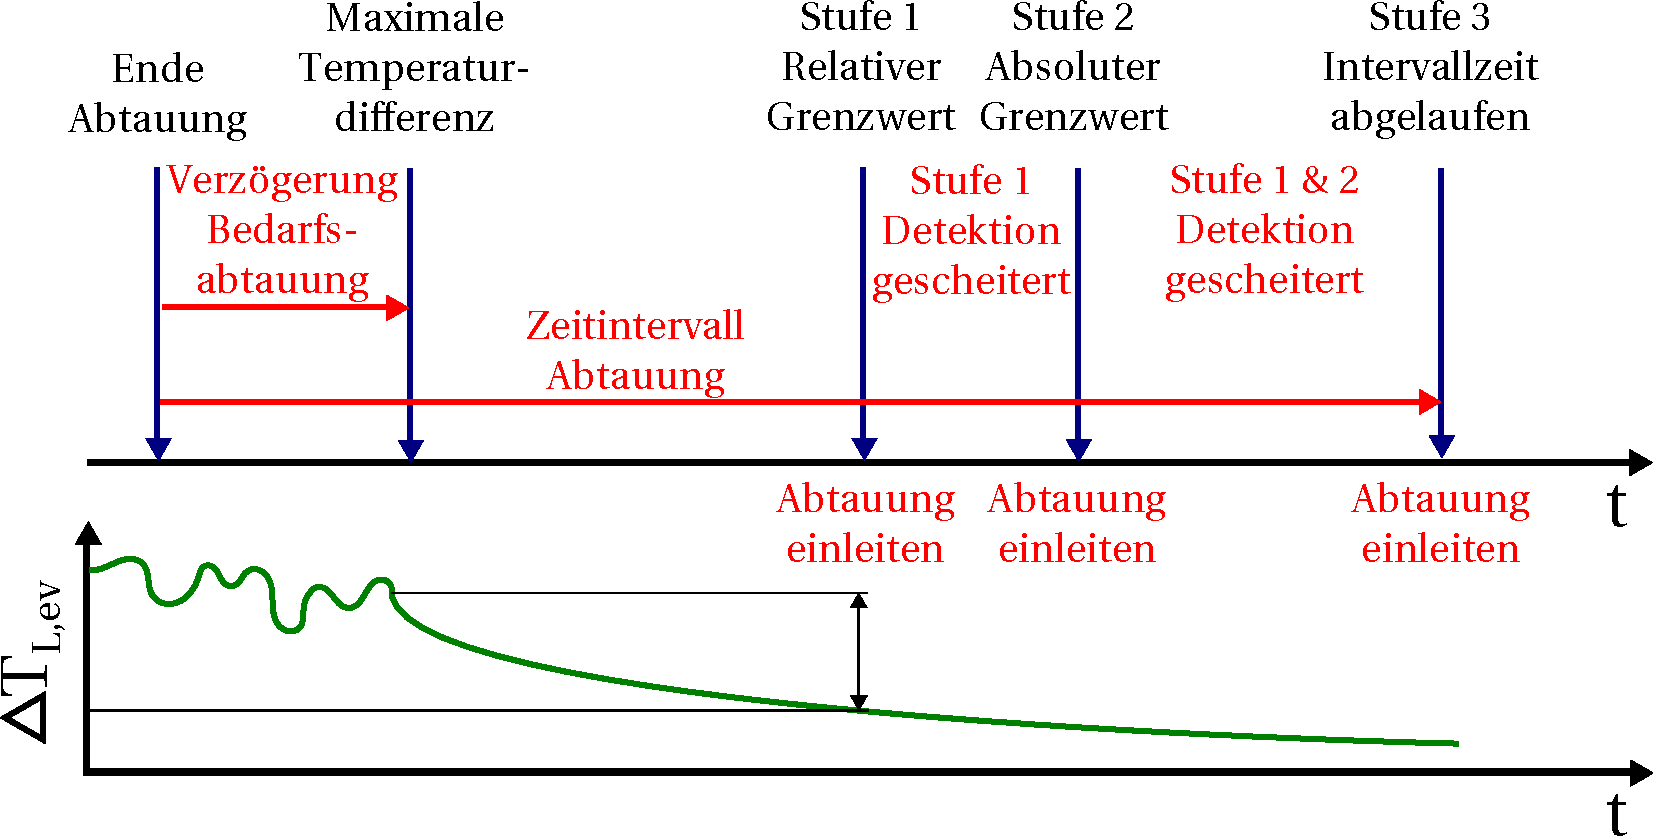
\includegraphics[scale=0.54]{Pictures/defrostintervall.pdf}
\caption{Auslösestufen der bedarfsgerechten Abtauung.}
\label{fig:bedarfsgerechteAbtauung}
\end{figure}

Im Folgenden wird die Temperaturdifferenz der Luft über den Verdampfer genauer betrachtet um Rückschlüsse auf das Regelverhalten der Steuerungssoftware ziehen zu können. Diese ist über einen Kühlzyklus in Abbildung~\ref{fig:deltaTLuftevap51} dargestellt. Auf der x-Achse ist die Zeit in $h$ und auf der y-Achse die Temperaturdifferenz in $K$ aufgetragen. Es ist zu erkennen, dass diese entgegen der Erwartungen mit fortschreitender Zeit ansteigt. Da die Temperaturdifferenz nicht sinkt kann auch kein eingestellter Grenzwert unterschritten werden. Infolgedessen findet keine Einleitung der Abtauung durch die ersten beiden Stufen der Regelung statt. 

\begin{figure}[h!]
\centering
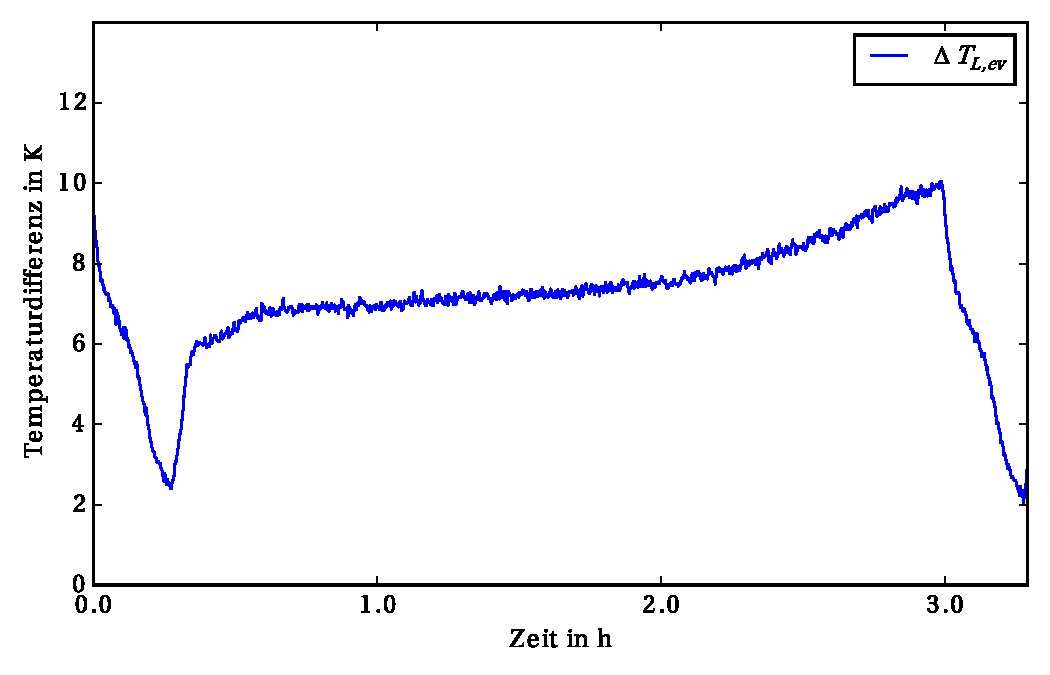
\includegraphics[scale=0.8]{Pictures/51/delTaT_evap1.pdf}
\caption{Temperaturdifferenz der Luft am Verdampfer bei einem 3h Abtauintervall.}
\label{fig:deltaTLuftevap51}
\end{figure}

Die Regelung der bedarfsgerechten Abtauung basiert auf der Annahme, dass die Temperaturdifferenz der Luft kleiner wird. Dies hat den folgenden Grund:
Während eines Kühlzyklus sammelt sich aufgrund der unter dem Tau- und Gefrierpunkt liegenden Temperatur der Verdampferoberfläche und der hohen relativen Luftfeuchtigkeit Kondensat, welches daraufhin gefriert. Wegen der stetig dicker werdenden Eisschicht entsteht ein zusätzlicher Wärmeleitwiderstand. Dieser verkleinert den Wärmedurchgangskoeffizienten $k$ entsprechend Gleichung~\ref{eq:UA}. Dies hat gemäß Gleichung~\ref{eq:4} eine Reduzierung der übertragenen Wärme zur Folge. Die Temperaturdifferenz wird kleiner, da die Austrittstemperatur der Luft infolgedessen höher ist. \newline
Abbildung~\ref{fig:deltaTLuftevap50} zeigt die Temperaturdifferenz der Luft bei der Vergleichsuntersuchung mit einem \unit{4}{\hour} Abtauintervall. Es ist zu erkennen, dass wie bei der nachfolgenden Untersuchung die Temperaturdifferenz zunächst ansteigt. Jedoch beginnt diese bei circa \unit{3.7}{\hour} rapide abzusinken. Zu diesem Zeitpunkt ist der Effekt der Eisbildung detektierbar und eine Einleitung der Abtauung durch die ersten beiden Stufen möglich. Dies wird jedoch durch das kurze Abtauintervall und durch die zunächst ansteigende Temperaturdifferenz verhindert. \newline 
Eine Untersuchung der Ein- und Austrittstemperaturen der Luft am Verdampfer lässt Rückschlüsse auf das Verhalten der Temperaturdifferenz zu.
Abbildung~\ref{fig:TLuftevap51} stellt diese zeitlich über das \unit{3}{\hour} Abtauintervall der Untersuchung der bedarfsgerechten Abtauung dar.
Es ist zu erkennen, dass die Austrittstemperatur der Luft nach Beginn des Kühlzyklus  langsam von circa \unit{2}{\celsius} auf bis zu \unit{-1}{\celsius} absinkt. Nach etwa \unit{2.5}{\hour} sinkt die Temperatur schneller ab. Währenddessen bleibt die Eintrittstemperatur in den Verdampfer mit etwa \unit{8}{\celsius} bis \unit{9}{\celsius} nahezu konstant. Tendenziell ist eine geringe Erhöhung der Temperatur zu erkennen. Das Absinken der Austrittstemperatur der Luft ist direkt abhängig von deren Eintrittstemperatur sowie der Verdampfungstemperatur des Kältemittels.

\begin{figure}[h]
\centering
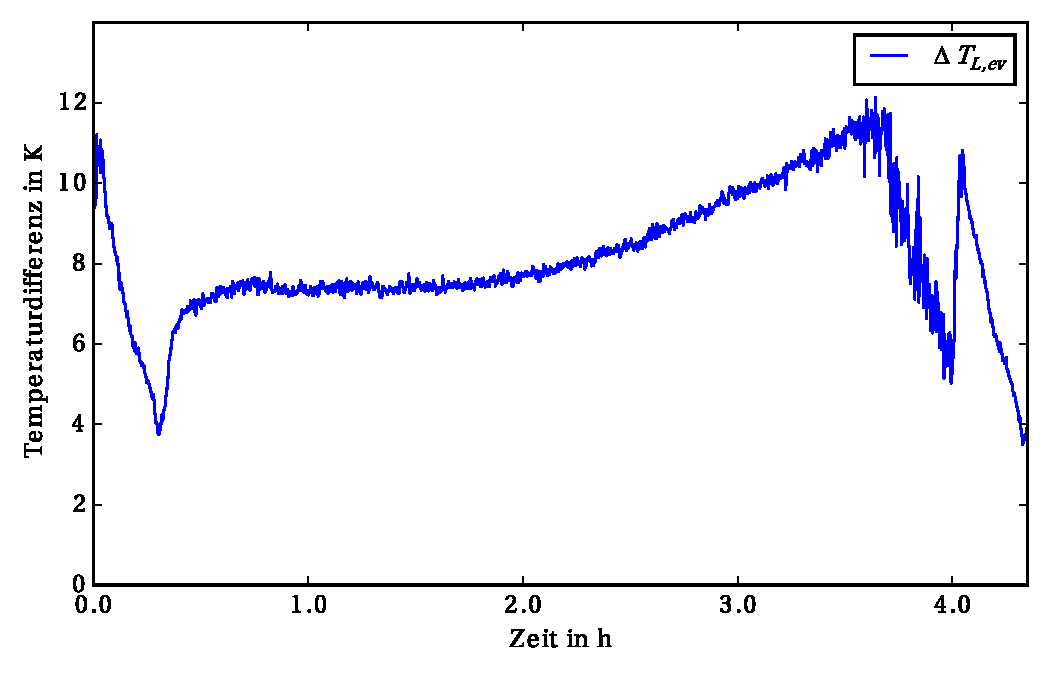
\includegraphics[scale=0.8]{Pictures/50/delTaT_evap1.pdf}
\caption{Temperaturdifferenz der Luft am Verdampfer bei einem 4h Abtauintervall.}
\label{fig:deltaTLuftevap50}
\end{figure}

In Abbildung~\ref{fig:Tevap51} ist die Verdampfungstemperatur des Kältemittels für alle drei Kältekreise zeitlich dargestellt. Nach Beginn des Kühlzyklus betragen die Verdampfungstemperaturen etwa \unit{-6}{\celsius} und fallen stetig bis auf \unit{-10}{\celsius}. Nach etwa \unit{2.5}{\hour} sinken die Temperaturen schneller ab. Aus dem Vergleich der Abbildungen~\ref{fig:TLuftevap51} und \ref{fig:Tevap51} lässt sich schließen, dass aufgrund der Ähnlichkeit beider Temperaturgraphen die Austrittstemperatur der Luft proportional von der Verdampfungstemperatur abhängig ist.\newline Es ist zu erwarten, dass sich die Eintrittstemperatur der Luft proportional zu deren Austrittstemperatur verhält. Diese Annahme wird durch die tendenziell steigende Eintrittstemperatur widerlegt. Es ist zu vermuten, dass durch die sinkende Austrittstemperatur der Luft am Auslassgitter des Kühlmöbels, infolge einer Veränderung des Wärmeübergangs durch Konvektion, die Induktionsrate der warmen Kammerluft erhöht wird. Bei sinkender Austrittstemperatur vermischt sich die Luft des Schleiers mit einer größeren Menge der Kammerluft, wodurch die Luft des Kühlmöbels stärker erhitzt wird.
Dieser Effekt ist eine mögliche Erklärung für die steigende Temperaturdifferenz der Luft.

\begin{figure}[h!]
\centering
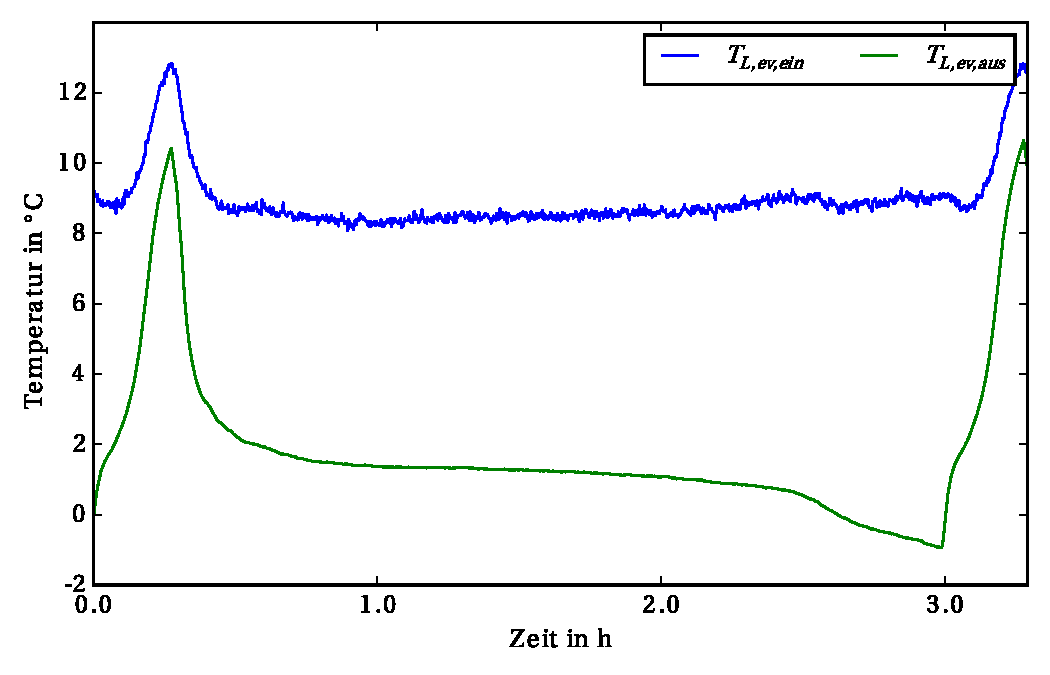
\includegraphics[scale=0.8]{Pictures/51/T_air,evap1.pdf}
\caption{Ein- und Austrittstemperaturen der Luft am Verdampfer bei einem 3h Abtauintervall.}
\label{fig:TLuftevap51}
\end{figure}

\begin{figure}[h!]
\centering
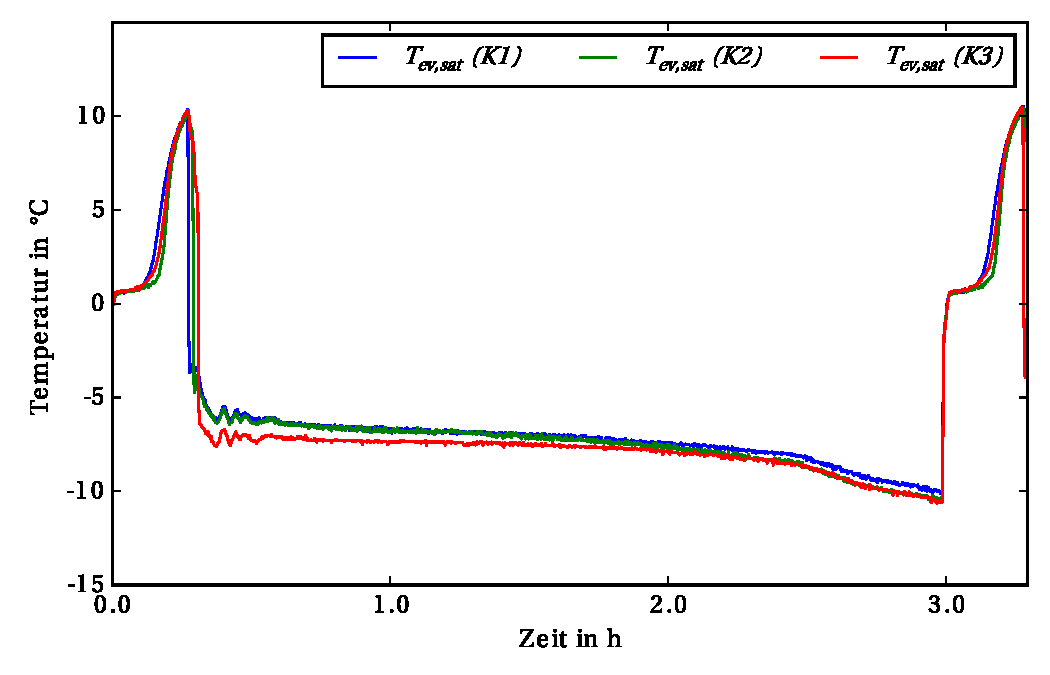
\includegraphics[scale=0.8]{Pictures/51/Tsats_K1K2K3lastCycle1.pdf}
\caption{Verdampfungstemperaturen der drei Kältekreise bei einem 3h Abtauintervall.}
\label{fig:Tevap51}
\end{figure}



\begin{figure}[h!]
\centering
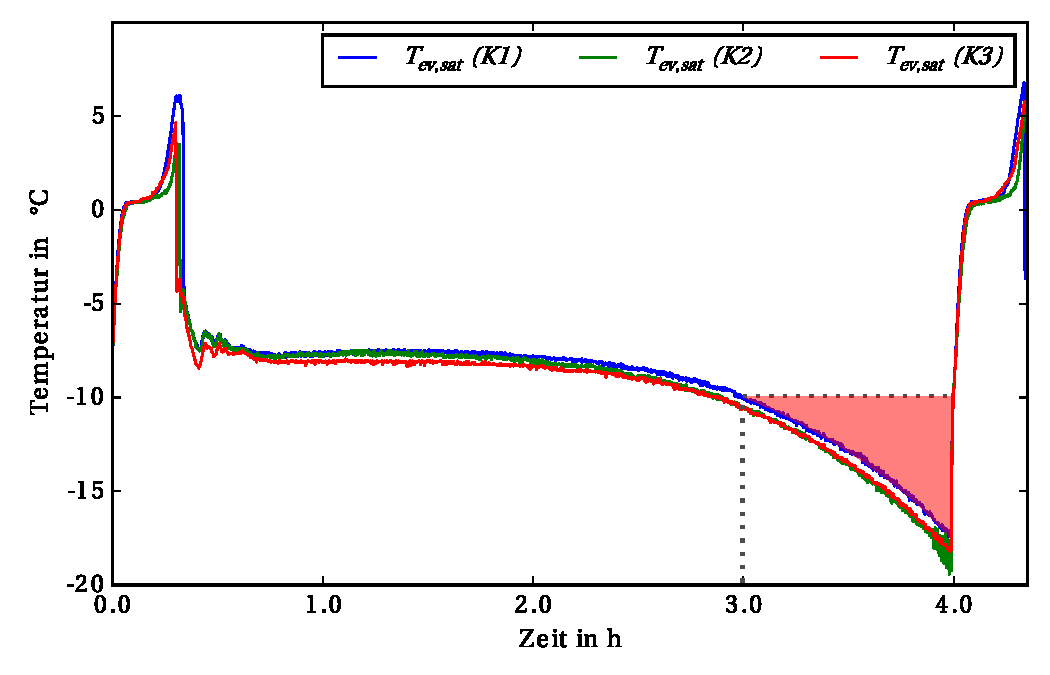
\includegraphics[scale=0.8]{Pictures/50evaploss1.pdf}
\caption{Verdampfungstemperaturen der drei Kältekreise bei einem 4h Abtauintervall.}
\label{fig:SinkenVerdampfung4h3h}
\end{figure}

\begin{figure}[h!]
\centering
%\def\svgwidth{120mm}
%\input{Pictures/50powerloss1.pdf_tex}
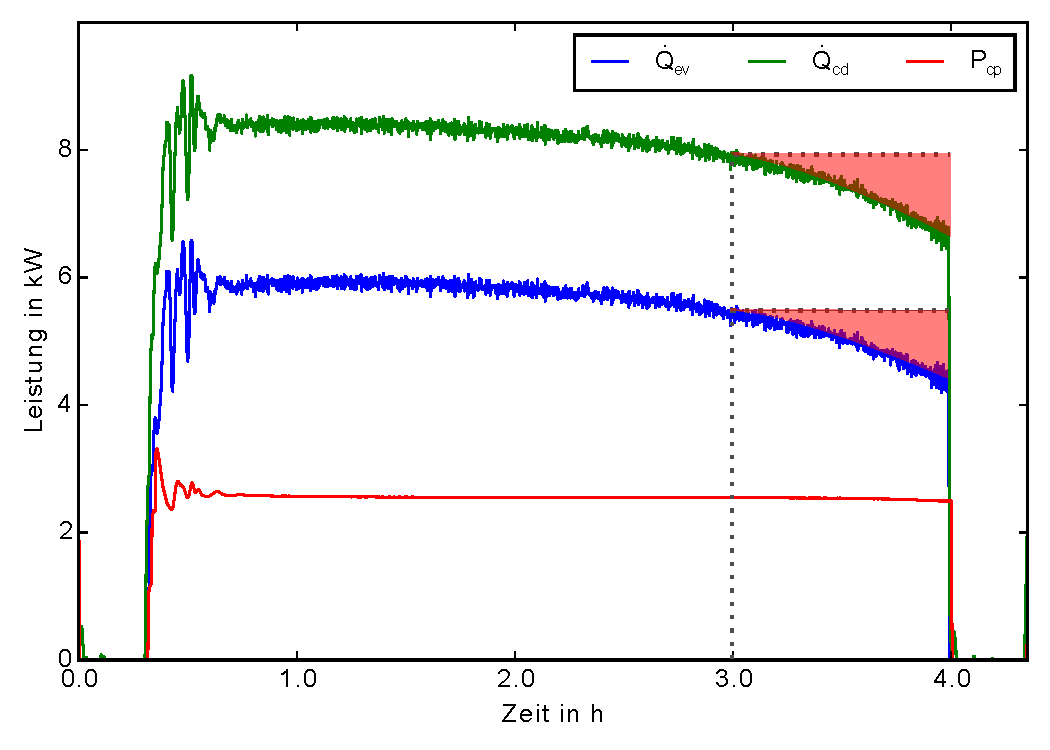
\includegraphics[scale=0.8]{Pictures/50powerloss.pdf}
\caption{Elektrische und thermische Leistungen bei einem 4h Abtauintervall.}
\label{fig:Leistungsverlust4h3h}
\end{figure}



Die Ergebnisse aus Abschnitt~\ref{sec:Abtauintervalle} zeigen eine Effizienzsteigerung durch eine Verkürzung des Abtauintervalls auf \unit{3}{\hour}. Um diesen Effekt zu untersuchen werden die Verdampfungstemperaturen und die Leistungen grafisch betrachtet.
In Abbildung~\ref{fig:SinkenVerdampfung4h3h} sind die Verdampfungstemperaturen der Untersuchung des \unit{4}{\hour} Abtauintervalls zeitlich über einen Kühlzyklus dargestellt. Von Beginn des Zyklus bis zu einem Zeitpunkt von etwa \unit{2}{\hour} bleiben die Temperaturen mit circa \unit{-7}{\celsius} konstant. Anschließend beginnen die Temperaturen zu fallen. Ab \unit{3}{\hour} sinken die Temperaturen sehr stark auf bis zu \unit{-18}{\celsius}.
Abbildung~\ref{fig:Leistungsverlust4h3h} stellt die elektrische Leistungsaufnahme der Verdichter und die thermischen Leistungen der Wärmeübertrager desselben Zyklus zeitlich dar. Während die elektrische Leistungsaufnahme konstant bleibt sinken die thermischen Leistungen wie die Verdampfungstemperatur ab einem Zeitpunkt von \unit{3}{\hour} stark ab. In beiden Diagrammen ist die Reduktion der jeweiligen Werte im Bereich zwischen \unit{3}{\hour} und \unit{4}{\hour} rot gekennzeichnet. \newline
Da diese Betrachtung unabhängig von der Temperatur der Eintrittsluft ist kann der Effekt der Eisbildung früher als bei einer Betrachtung der Temperaturdifferenz detektiert werden. Eine Verkürzung des Abtauintervalls verhindert ein starkes Absinken der thermischen Leistungen und der Verdampfungstemperaturen. Da die Werte in Tabelle~\ref{tab:Vergleich4h3h} über die letzten \unit{75}{\%} eines Zyklus gemittelt sind, sind die des \unit{4}{\hour} Abtauintervalls entsprechend geringer.

Durch die Änderung des Abtauintervalls von \unit{4}{\hour} auf \unit{3}{\hour} wird der EER um \unit{5.6}{\%} von \unit{2.14}{} auf \unit{2.26}{} erhöht.















\section{Verdichter}
\label{sec:VerdichterAnalyse}

In diesem Abschnitt wird das Verhalten des Systems auf Basis der Ergebnisse aus Abschnitt~\ref{sec:Verdichter} analysiert und der Tausch der Verdichter bewertet. 
Aufgrund der erzielten höheren Kondensationsleistung und der daraus resultierenden größeren Enthalpiedifferenz erreicht das Kältemittel einen niedrigeren Dampfgehalt. Bei Drosselung durch das Expansionsventil bleibt die Enthalpie nahezu konstant. Der erzielte Flashgasanteil hinter dem Ventil ist folglich ebenfalls geringer. Dadurch wird ein Verdampfungsenthalpiegewinn erzielt, wie beim Vergleich der Diagramme~\ref{fig:logph51} und \ref{fig:logph54} erkennbar ist. Trotz eines niedrigeren Kältemittelmassenstroms wird an den Wärmeübertragern mehr Wärme übertragen. Bei Reduzierung des Massenstroms ist immer ein Anstieg der Enthalpiedifferenz zu beobachten. Gemäß Gleichung~\ref{eq:4} bleibt so die Leistung konstant. \newline
Nach Gleichung~\ref{eq:14} wird der Druckabfall über den Verdampfer gleichermaßen durch den Dampfanteil und den Kältemittelmassenstrom beeinflusst. Eine Reduktion beider Größen hat, wie in den Messwerten von Kreis 2 und 3 in Tabelle~\ref{tab:VergleichVerdichter} erkennbar, eine Reduktion des Druckabfalls über den Verdampfer zur Folge. Das in Abschnitt~\ref{subsec:Das Modell} beschriebene Modell zeigt, dass der Druckabfall auf einem höheren Druckniveau größer ist. Demnach ist der in Kreis~1 leicht erhöhte Druckabfall durch die geringe Änderung von Dampfanteil und Massenstrom bei gleichzeitig minimaler Erhöhung des Verdampfungsdrucks zu erklären. \newline
Die Abweichung des Systemverhaltens von den Herstellerdaten lässt sich dadurch erklären, dass diese bei einem Betriebspunkt mit \unit{0}{\kelvin} Unterkühlung gelten. Da keine Unterkühlung erzielt und ein hoher Dampfanteil vorhanden ist sind die Daten nicht vergleichbar. Die tendenzielle Änderung zu einem höheren Massenstrom bei geringerer elektrischer Leistungsaufnahme ist durch eine Änderung des Betriebspunkts im Verdichterkennfeld zu erklären. Bei einem typischen Verdichterkennfeld,ist das Druckverhältnis über dem Massenstrom aufgetragen. Eine Reduktion des Massenstromes bei ähnlichem Druckverhältnis sowie konstanter Drehzahl kann, je nach Betriebspunkt, eine Reduktion des isentropen Wirkungsgrads zur Folge haben \cite{Wilke.2005}. 
Dies kann zu einer Erhöhung der elektrischen Leistungsaufnahme und der Wärmeabgabe führen, wodurch die Verflüssigungsleistung erhöht wird. Diesem Verhalten liegt eine andere Leistungskurve des Kupfermotors gegenüber dem Aluminiummotor zugrunde. Die Herstellerdaten versprechen tendenziell eine Erhöhung der Verdichterkälteleistung. Ein Zusammenspiel dieser Effekte resultiert in dem gegenwärtigen Betriebspunkt.  \newline
Der Betrieb mit der Standardausführung des Scrollverdichters ZB09KAU-TFD wirkt sich unter den gegenwärtigen Prüfbedingungen sowohl leistungs- als auch leicht effizienzsteigernd aus. Gegenüber dem Hybridmodell wird kein eindeutiger EER-Gewinn erzielt.


\section{Änderung der Verdampferschaltung}
\label{sec:Änderung der Verdampferschaltung1}


In diesem Unterkapitel werden die Ergebnisse aus Abschnitt~\ref{sec:Änderung der Verdampferschaltung} analysiert und hinsichtlich deren Auffälligkeiten untersucht.

\subsection{Vergleich zwischen Verdampfern}
\label{subsec:Vergleich zwischen Verdampfern_1}

In diesem Abschnitt wird der Effekt des Umstiegs vom zweireihigen AHT-Verdampfer zum vierreihigen LIDL-Verdampfer auf das Systemverhalten untersucht. Es ist zu untersuchen warum die Leistung des Systems verringert wird und die Produkttemperaturen ansteigen. 
Mit Umstieg auf den LIDL-Verdampfer ist zunächst ein Anstieg der Überhitzung sowie eine Abweichung der von den Expansionsventilen erfassten Überhitzung von der messtechnisch erfassten Überhitzung auffällig. Durch das vierreihige Design wird eine bessere Umströmung der Verdampferrohre von der Luft erzielt, wodurch der Wärmeübertragungskoeffizient $\alpha_{L}$ erhöht wird. Dies resultiert in einer Erhöhung des $k$-Werts und damit, gemäß Gleichung~\ref{eq:4}, in einer Erhöhung des übertragenen Wärmestroms. Durch die bessere Wärmeübertragung steigt die Überhitzung an, worauf das Expansionsventil mit einer Erhöhung des Öffnungsgrades reagiert. Während des Betriebs mit dem neuen Verdampfer sind die Expansionsventile in den drei Kreisen vollständig geöffnet. Dies ist ersichtlich aus der starken Erhöhung des Kältemittelmassenstroms und aus der über dem Sollwert liegenden Überhitzung. Dies ist jedoch keine Erklärung für die beobachteten Abweichungen der erfassten Überhitzungen beim Betrieb mit dem neuen Verdampfer. Diese betragen etwa \unit{1}{\kelvin} bis \unit{2}{\kelvin}. Es ist möglich, dass durch die andere Wärmeübertragungs- sowie Strömungscharakteristik des neuen Verdampfers zu einem anderen Regelverhalten des Expansionsventil führt \cite{Winter.2012}. Eine weitere Erklärung könnte sein, dass die internen Berechnungen der Expansionsventile, denen Koeffizienten zugrunde liegen, dadurch fehlerhaft sind \cite{EmersonClimateTechnologies.2016}. Mit dem höheren Kältemittelmassenstrom geht ein Anstieg des Wassermassenstroms am Kondensator sowie eine Reduktion der Enthalpiedifferenz am Verflüssiger einher. Dies führt wiederum, durch den höheren Dampfanteil, zu einer Reduktion der Verdampferleistung. Zudem steigt mit dem Massenstrom der Druckabfall über den Verdampfer an. Die veränderte Wärmeübertragungscharakteristik hat einen höheren Verdampfungsdruck zur Folge, der mit einer höheren Verdampfungstemperatur einhergeht. Diese Effekte resultieren in einer höheren Luftauslasstemperatur und damit in einer höheren Durchschnittsprodukttemperatur. \newline
Aus dem Systemverhalten lässt sich somit schließen, dass die Füllmenge nicht ausreichend groß ist, um eine Überhitzungsregelung ermöglichen zu können. Eine höhere Füllmenge hätte ein höheres Druckniveau sowie eine damit verbundene höhere Verdampfungstemperatur zur Folge. Aufgrund der geringeren Temperaturdifferenz zur Luft würde weniger Wärme übertragen werden, wodurch die Überhitzung des Kältemittels sinken würde. Das Expansionsventil reagiert folglich mit einer Reduktion des Öffnungsgrads. Um in einen regelbaren Bereich der Überhitzung zu gelangen und ein stabiles Systemverhalten zu generieren wird der Sollwert der Überhitzung in nachfolgenden Untersuchungen auf \unit{13}{\kelvin} eingestellt. 



\subsection{Modellgestützter Vergleich der Verschaltungen V1 und V2}
\label{subsec:Modellgestützter Vergleich der Verschaltungen V1 und V2_1}

In diesem Abschnitt werden die Ergebnisse der Simulation sowie das Verhalten des Systems bei Änderung der Verschaltung der Verdampferrohre analysiert und hinsichtlich des Zieles der thermischen Leistungssteigerung bewertet.
Die Ursache für die im Vergleich viel tieferen Temperaturen ist die geringe relative Luftfeuchtigkeit.
Für die Validierung des Modells sind Untersuchungen bei \unit{0}{\%} r.F. in der Klimakammer notwendig. Tatsächlich erreichbar sind \unit{5}{\%} bis \unit{25}{\%} r.F.. Da bei diesen trotzdem sehr niedrigen Werten kaum Kälteleistung für die Kondensation des Wassers aus der Luft benötigt wird, ist mehr Kälteleistung zur sensiblen Wärmeaufnahme der Luft verfügbar. Dies resultiert in einer tieferen Luftauslasstemperatur. Durch die sinkenden Temperaturen sinken ebenfalls Verdampfungsdruck und Verdampfungstemperatur. Das Modell zeigt, dass der verursachte Druckabfall auf einem niedrigeren Druckniveau ebenfalls niedriger ist. \newline
Die Ergebnisse der Simulation zeigen eine große Abweichung des errechneten Druckabfalls  zu den erfassten Messdaten. Die Berechnungsmethode verspricht laut Quellen eine Genauigkeit von $\pm 30 \%$. Die Abweichung unter gegenwärtigen Bedingungen beträgt etwa \unit{42}{\%} bis \unit{44}{\%} . Allerdings ist die Berechnung des Druckabfalls auf einem höheren Druckniveau sehr genau. Das Modell wurde basierend auf Messdaten aus Untersuchungen bei \unit{60}{\%} r.F. berechnet. Dabei wurden Genauigkeiten von \unit{10}{\%} bis \unit{20}{\%} erzielt. Dies lässt darauf schließen, dass die Gleichungen zur Berechnung des Druckabfalls einen bestimmten Gültigkeitsbereich besitzen, der unter den gegenwärtigen Untersuchungsbedingungen verlassen wird. \newline
Trotz ungenauer Berechnung des Druckabfalls sind die Berechnungen der Temperaturen und der Leistungen sehr genau. Das liegt daran, dass die Parameter des Modells, die Wärmeübergangskoeffzienten $\alpha_L$, $\alpha_{KM}$ und $\alpha_{KM,SH}$, manuell so angepasst wurden, dass der errechnete dem messtechnisch erfassten Temperaturverlauf entspricht. Dies hat zur Folge, dass das Modell mit den aktuellen Parameterwerten nicht allgemeingültig ist. \newline
Der durch die Änderung der Verdampferschaltung sichtbare Effekt in der Kälteleistung wird ebenfalls durch den zu gering berechneten Druckabfall beeinflusst. Der durch das Modell berechnete Kälteleistungsgewinn ist nur halb so groß wie der tatsächlich erzielte. Dadurch, dass der berechnete Druckabfall zu niedrig ist, ist auch die Änderung des Druckabfalls nach Änderung der Verschaltung proportional niedriger. Dies spiegelt sich in den erzielten Verdampfungstemperaturen und damit in der Kälteleistung wider.
Aufgrund dessen ist zu vermuten, dass der Effekt der Verschaltungsänderung auf die Leistung, während den Untersuchungen bei \unit{60}{\%} r.F., noch deutlicher wird, da der Druckabfall wegen des höheren Druckniveaus ebenfalls höher ist. Durch das Modell wird neben dem Leistungsgewinn ein ebenfalls gesteigerter Druckabfall berechnet. Die Ursache dessen liegt im höheren Wärmestrom. Dadurch, dass das Kältemittel durch die veränderte Verschaltung mehr Wärme aufnimmt, wechselt es schneller den Aggregatzustand. Zwischen gasförmigem und flüssigem Kältemittel stellt sich ein Geschwindigkeitsschlupf ein, da gasförmiges Kältemittel aufgrund dessen geringer Dichte schneller strömt. Stärkere Reibungseffekte erhöhen deshalb den Reibungsdruckabfall. Das Kältemittel hat zu einem früheren Zeitpunkt als in der vorherigen Verschaltung dieselbe Geschwindigkeit. Es werden in jeder Zelle des Modells höhere Geschwindigkeiten berechnet. Da der Druckabfall, gemäß Gleichung~\ref{eq:14} quadratisch zur Geschwindigkeit steigt ist der Druckabfall in Verschaltung~V2 größer. \newline
Bei der Betrachtung der Temperaturprofile der Luft in den Abbildungen~\ref{fig:SimTempV1} und \ref{fig:SimTempV2}, ist fast kein Unterschied ersichtlich. Aus den Temperaturprofilen des Kältemittels ist der Effekt durch die Umkehr der Fließrichtung des Kältemittels ersichtlich. Diese gleichen nun denen eines reinen Gegenstromwärmeübertragers. Zudem ist eine höhere Überhitzung in Verschaltung~V2 zu erkennen. Diese wird durch den von V2 erzielten Leistungsgewinn verursacht. Im realen System würde dies durch die Überhitzungsregelung kompensiert werden und in einem geringeren Massenstrom resultieren. Ein steilerer Druckgradient geht mit einem steileren Temperaturgradienten einher, was eine Verstärkung des Effekts der Verschaltungsänderung verursacht. Wie zuvor erwähnt ist dies bei Normbedingungen zu erwarten. \newline
Die erfassten Messwerte bestätigen die Tendenz des Modells. Mit etwa \unit{35}{\watt} bis \unit{55}{\watt} Kälteleistungsgewinn je Kältekreis wird ein Gesamtkälteleistungsgewinn von \unit{140}{\watt} erzielt. Bei gleichzeitiger Reduktion der elektrischen Leistungsaufnahme resultiert dies in einem höheren EER. Durch den bei höherer Verflüssigungsleistung geringeren Kältemittelmassenstrom wird die Enthalpiedifferenz von Verdampfer und Kondensator erhöht. Zudem werden in diesem Zustand Dampfanteile von \unit{100}{\%} und daraus resultierende Unterkühlungen von \unit{3}{\kelvin} bis \unit{4}{\kelvin} realisiert.
Bei steigender Überhitzung reagiert das Expansionsventil, um diese zu kompensieren, mit einer Erhöhung des Öffnungsgrades und damit einer Steigerung des Kältemittelmassenstrom. Die Untersuchungen zeigen aber einen niedrigeren Massenstrom und eine geringfügig höhere Überhitzung. Dies ist wahrscheinlich auf eine Verschiebung des Betriebspunktes der Verdichter zurückzuführen. Bei einem Verdichterkennfeld ist das Druckverhältnis über dem Massenstrom aufgetragen \cite{Wilke.2005}. Ein, durch gesteigerten Druckabfall, zunehmendes Druckverhältnis kann bei gleicher Motordrehzahl zu einem geringeren Massenstrom führen und zu einer Reduktion des isentropen Wirkungsgrades. \newline
Mittels des Modells wird durch die Verschaltungsänderung eine Erhöhung der thermischen Leistungen und des Druckabfalls vorausgesagt, was durch die Untersuchungen bestätigt wird. Dies resultiert in einer Effizienzsteigerung von \unit{4}{\%}. 

\subsection{Vergleich der Verschaltungen V1 und V2}
\label{subsec:Vergleich der Verschaltungen V1 und V2_1}

In diesem Abschnitt werden die in Abschnitt~\ref{subsec:Vergleich der Verschaltungen V1 und V2_1} beschriebenen Untersuchungsergebnisse von Verschaltung~V1 und V2 bei \unit{60}{\%} r.F. analysiert.
Das Druck- und Temperaturniveau ist bei dieser Untersuchung höher als das der vorausgehenden Untersuchung. Durch den höheren Anteil an Feuchtigkeit in der Luft wird ein Teil der Kälteleistung dazu benötigt diese zu kondensieren. Deswegen wird die Luft nicht so stark abgekühlt wie zuvor und die Verdampfungsdrücke und -temperaturen sind entsprechend höher. Die Verdampferleistungen in beiden Verschaltungen sind bei feuchter Luft höher als bei trockener Luft, da feuchte Luft eine höhere Wärmeleitfähigkeit besitzt und damit gemäß der Gleichungen~\ref{eq:4}, \ref{eq:UA} und \ref{eq:28} mehr Wärme übertragen wird \cite{Lasance.2003}. Der Effekt auf die Leistungssteigerung des Verdampfers ist mit \unit{140}{\watt} Leistungsgewinn genauso groß wie in der vorigen Untersuchung. Damit ist dieser wider der Erwartung, dass der steigende Druckabfall die Verdampferleistung vergrößert, nicht größer als unter trockenen Bedingungen. Der durch die Änderung der Verschaltung verursachte Druckabfall ist zwar gegenüber der Untersuchung bei \unit{0}{\%} r.F. bedingt durch den höheren Massenstrom größer, allerdings führt dies nicht zu einem proportionalen Anstieg der Verdampferleistung sondern wird anderweitig vom System kompensiert. Dabei liegt die Begründung vermutlich in einer Verschiebung des Betriebspunkts im Kennfeld des Verdichters. Eine Erhöhung des Druckverhältnisses bedingt dabei eine Reduktion des Kältemittelmassenstroms.
Den Änderungen in den Messwerten liegen dieselben Ursachen zugrunde wie denen aus Abschnitt~\ref{subsec:Modellgestützter Vergleich der Verschaltungen V1 und V2_1}.
Durch Verschaltung~V2 wird ein Betriebspunkt erreicht in dem der Zustand des Kältemittels vor dem Expansionsventil sich genau auf der Siedelinie befindet. 
Dies ist erstrebenswert in Hinsicht auf den Schutz des Expansionsventils vor Schlägen von Gasblasen und auf dessen Regelverhalten. \newline
Mittels Verschaltung~V2 werden mit \unit{-0.47}{\celsius} minimaler und \unit{10.25}{\celsius} maximaler Produkttemperatur die bislang tiefsten Produkttemperaturen erzielt, wenn die Untersuchung bei \unit{0}{\%} r.F. nicht miteinbezogen wird. Diese werden durch die tiefere Verdampfungstemperatur und die Optimierung der Verschaltung generiert. Wegen des veränderten Überhitzungssollwerts sind die Ergebnisse nicht direkt mit denen vor dem Verdampfertausch vergleichbar.
Die Effizienzsteigerung beträgt unter feuchten Bedingungen \unit{3}{\%}, sodass ein vergleichsweise hoher EER von \unit{2.28}{} erzielt wird. 



\chapter{Zusammenfassung und Ausblick}
\label{cha:Zusammenfassung}

Im Rahmen dieser Arbeit wurden experimentelle Untersuchungen an einem vertikalen Supermarktkühlmöbel in einer Klimakammer durchgeführt, mit dem Ziel unter Veränderung günstiger Parameter eine thermische Leistungssteigerung herbeizuführen. Zur Untersuchung des Einflusses einer modifizierten Reihenfolge der Verdampferrohre wurde ein mathematisches Modell des Verdampfers entwickelt und anhand von Versuchsdaten validiert. \newline
Eine Durchführung der Untersuchungen nach Normbedingungen ist nur begrenzt möglich. Die Vorgabe einer einheitlichen Luftgeschwindigkeit zwischen \unit{0.1}{\metre\per\second} und \unit{0.2}{\metre\per\second} an drei Punkten über die Höhe der linken Außenkante des Kühlmöbels kann nicht eingehalten werden. Es ist ein Gradient von Geschwindigkeiten zwischen \unit{0.02}{\metre\per\second} und \unit{0.35}{\metre\per\second} messbar. Eine Reduktion der Lüfterleistung führt zu einer Annäherung der Werte in den Zielbereich. Allerdings führt dies zu einem Temperaturgradienten von \unit{2}{\kelvin} über die Höhe des Möbels und zu einer instabilen Regelung von Temperatur und relativer Luftfeuchtigkeit. Deswegen wurde für die nachfolgenden Untersuchungen ein Betrieb mit zwei Lüftern mit je \unit{30}{\%} ihrer Leistung beschlossen. \newline
Berechnungen um die im jeweiligen Öl gelöste Kältemittelmenge zu bestimmen ergeben, dass HATCOL~4467 gegenüber 3MAF in den Wärmeübertragern eine um \unit{5}{\%} geringere Löslichkeit besitzt. Dies entspricht maximal etwa \unit{1}{\gram} bis \unit{1.5}{\gram} je Kältekreis. Mittels eines Spülsystems wurde festgestellt, dass sich kein zurückgebliebenes Öl in den Kältekreisen befindet. Der Wechsel zu HATCOL~4467 führt zu einer Erhöhung der thermischen Leistungen. Allerdings geht dies einher mit einer EER-Reduzietung um \unit{3.2}{\%} da auch die elektrische Leistungsaufnahme reduziert wird. \newline
Die Regelung der Abtauung detektiert wegen einer steigenden Temperaturdifferenz über den Verdampfer keinen Abtaubedarf und löst diese deshalb nach dem vorgegebenen maximalen Intervall von \unit{3}{\hour} aus. Die steigende Temperaturdifferenz ist vermutlich auf eine Erhöhung der Induktionsrate des Luftschleiers mit der warmen Raumluft durch eine Veränderung des konvektiven Wärmestroms zurückzuführen. Ab einer Zeitmarke von etwa \unit{3}{\hour} werden die thermischen Leistungen sowie die Verdampfungstemperaturen, bedingt durch Eisbildung am Verdampfer stark reduziert. Eine Verkürzung des Abtauintervalls auf \unit{3}{\hour} verhindert dies und erzielt damit einen EER-Gewinn von \unit{5.6}{\%}. \newline
Ein Wechsel von der Hybrid- zur Standardausführung des Verdichtermodells ZB09KAU-TFD erhöht bedingt durch eine andere Motorkennlinie die Kondensator- und Verdampferleistungen um \unit{400}{\watt}. Da auch die elektrische Leistungsaufnahme steigt führt dies nur zu einem geringen EER-Anstieg von etwa \unit{0.9}{\%}.\newline
Ein Umstieg auf den vierreihigen LIDL-Verdampfer führt aufgrund dessen besserer Wärmeübertragungscharakteristik zu einem Kältemittelmangel. Dies wird kompensiert durch eine Erhöhung des Überhitzungssollwerts von \unit{8}{\kelvin} auf \unit{13}{\kelvin}. \newline
Mittels des Modells werden durch die Verschaltungsänderung ein Anstieg des Druckabfalls und eine Erhöhung der Kälteleistung berechnet. Diese Tendenz wird durch die Untersuchungsergebnisse bestätigt. Bei geringen Druckverhältnissen weicht der berechnete Druckabfall stark von den erfassten Messwerten ab, sodass das Modell einen eingeschränkten Gültigkeitsbereich besitzt. Die modifizierte Verschaltung generiert durch den Druckabfall und die daraus resultierende Reduktion der Verdampfungstemperatur ein Temperaturprofil, dass dem eines Gegenstromwärmeübertragers gleicht. Dadurch werden mit minimal \unit{-0.47}{\celsius}  und maximal \unit{10.25}{\celsius} die im Rahmen der Untersuchungen tiefsten Produkttemperaturen und ein EER von \unit{2.28}{} erzielt.
Alle durchgeführten Veränderungen erweisen sich somit als leistungssteigernd. \newline
Als weitere Maßnahme zur Leistungssteigerung bietet sich die Installation von Venturi-Verteilern an. Diese teilen den Massenstrom auf mehrere Verdampferrohre auf und reduzieren dadurch den Druckabfall. Eine Reduktion des aufzubringenden Druckverhältnisses führt zu einer Steigerung des isentropen Wirkungsgrades.


%\chapter{Technik/Methoden}
\label{cha:Technik}

\section{Das Kühlregal}
\label{sec:Das Kühlregal}

Der Mittelpunkt der durchgeführten Untersuchungen ist ein Kühlregal der Firma AHT.
Es umfasst auf einer Länge von \unit{3,75}{\metre} vier Regalböden um Produkte zu kühlen und auszustellen. Ein von oben herabfallender Luftschleier ermöglicht ein türloses Design des Regals. Die Kälteerzeugung wird, wie in Abbildung~\ref{fig:IDC150} ersichtlich, durch drei seperate Kältekreisläufe gewährleistet. Das verwendete Kältemittel ist Propan (R290). Jeder Kreis besitzt eine Füllmenge von \unit{150}{\gram}. Um die Füllmenge zu reduzieren wurden bereits vor Beginn der Untersuchungen kältetechnische Komponenten mit geringerem internen Volumen eingebaut. Die Verdichter sind ein Produkt der Firma Emerson. Im Rahmen der Untersuchungen kommen mehrere Modelle zum Einsatz. Drei Plattenwärmeübertrager der Firma SWEP dienen als Verflüssiger. Sie besitzen je 20 Platten und eine Nennleistung von je \unit{2,7}{\kilo\watt}. Die Expansionsventile der Firma Alco sind elektronisch regelbar und besitzen einen Temperatur- sowie Drucksensor in der Saugleitung. Die drei Kreisläufe durchlaufen mit je sechs Durchgängen einen gemeinsamen Verdampfer dessen Lamellenabstand \unit{5}{\milli\metre} beträgt. Sechs Lüftermotoren der Firma EBM Pabst saugen die Luft durch den Verdampfer mit einer konstanten Drehzahl von \unit{1400}{U\per\min}.

\begin{figure} %[!htb]
\centering
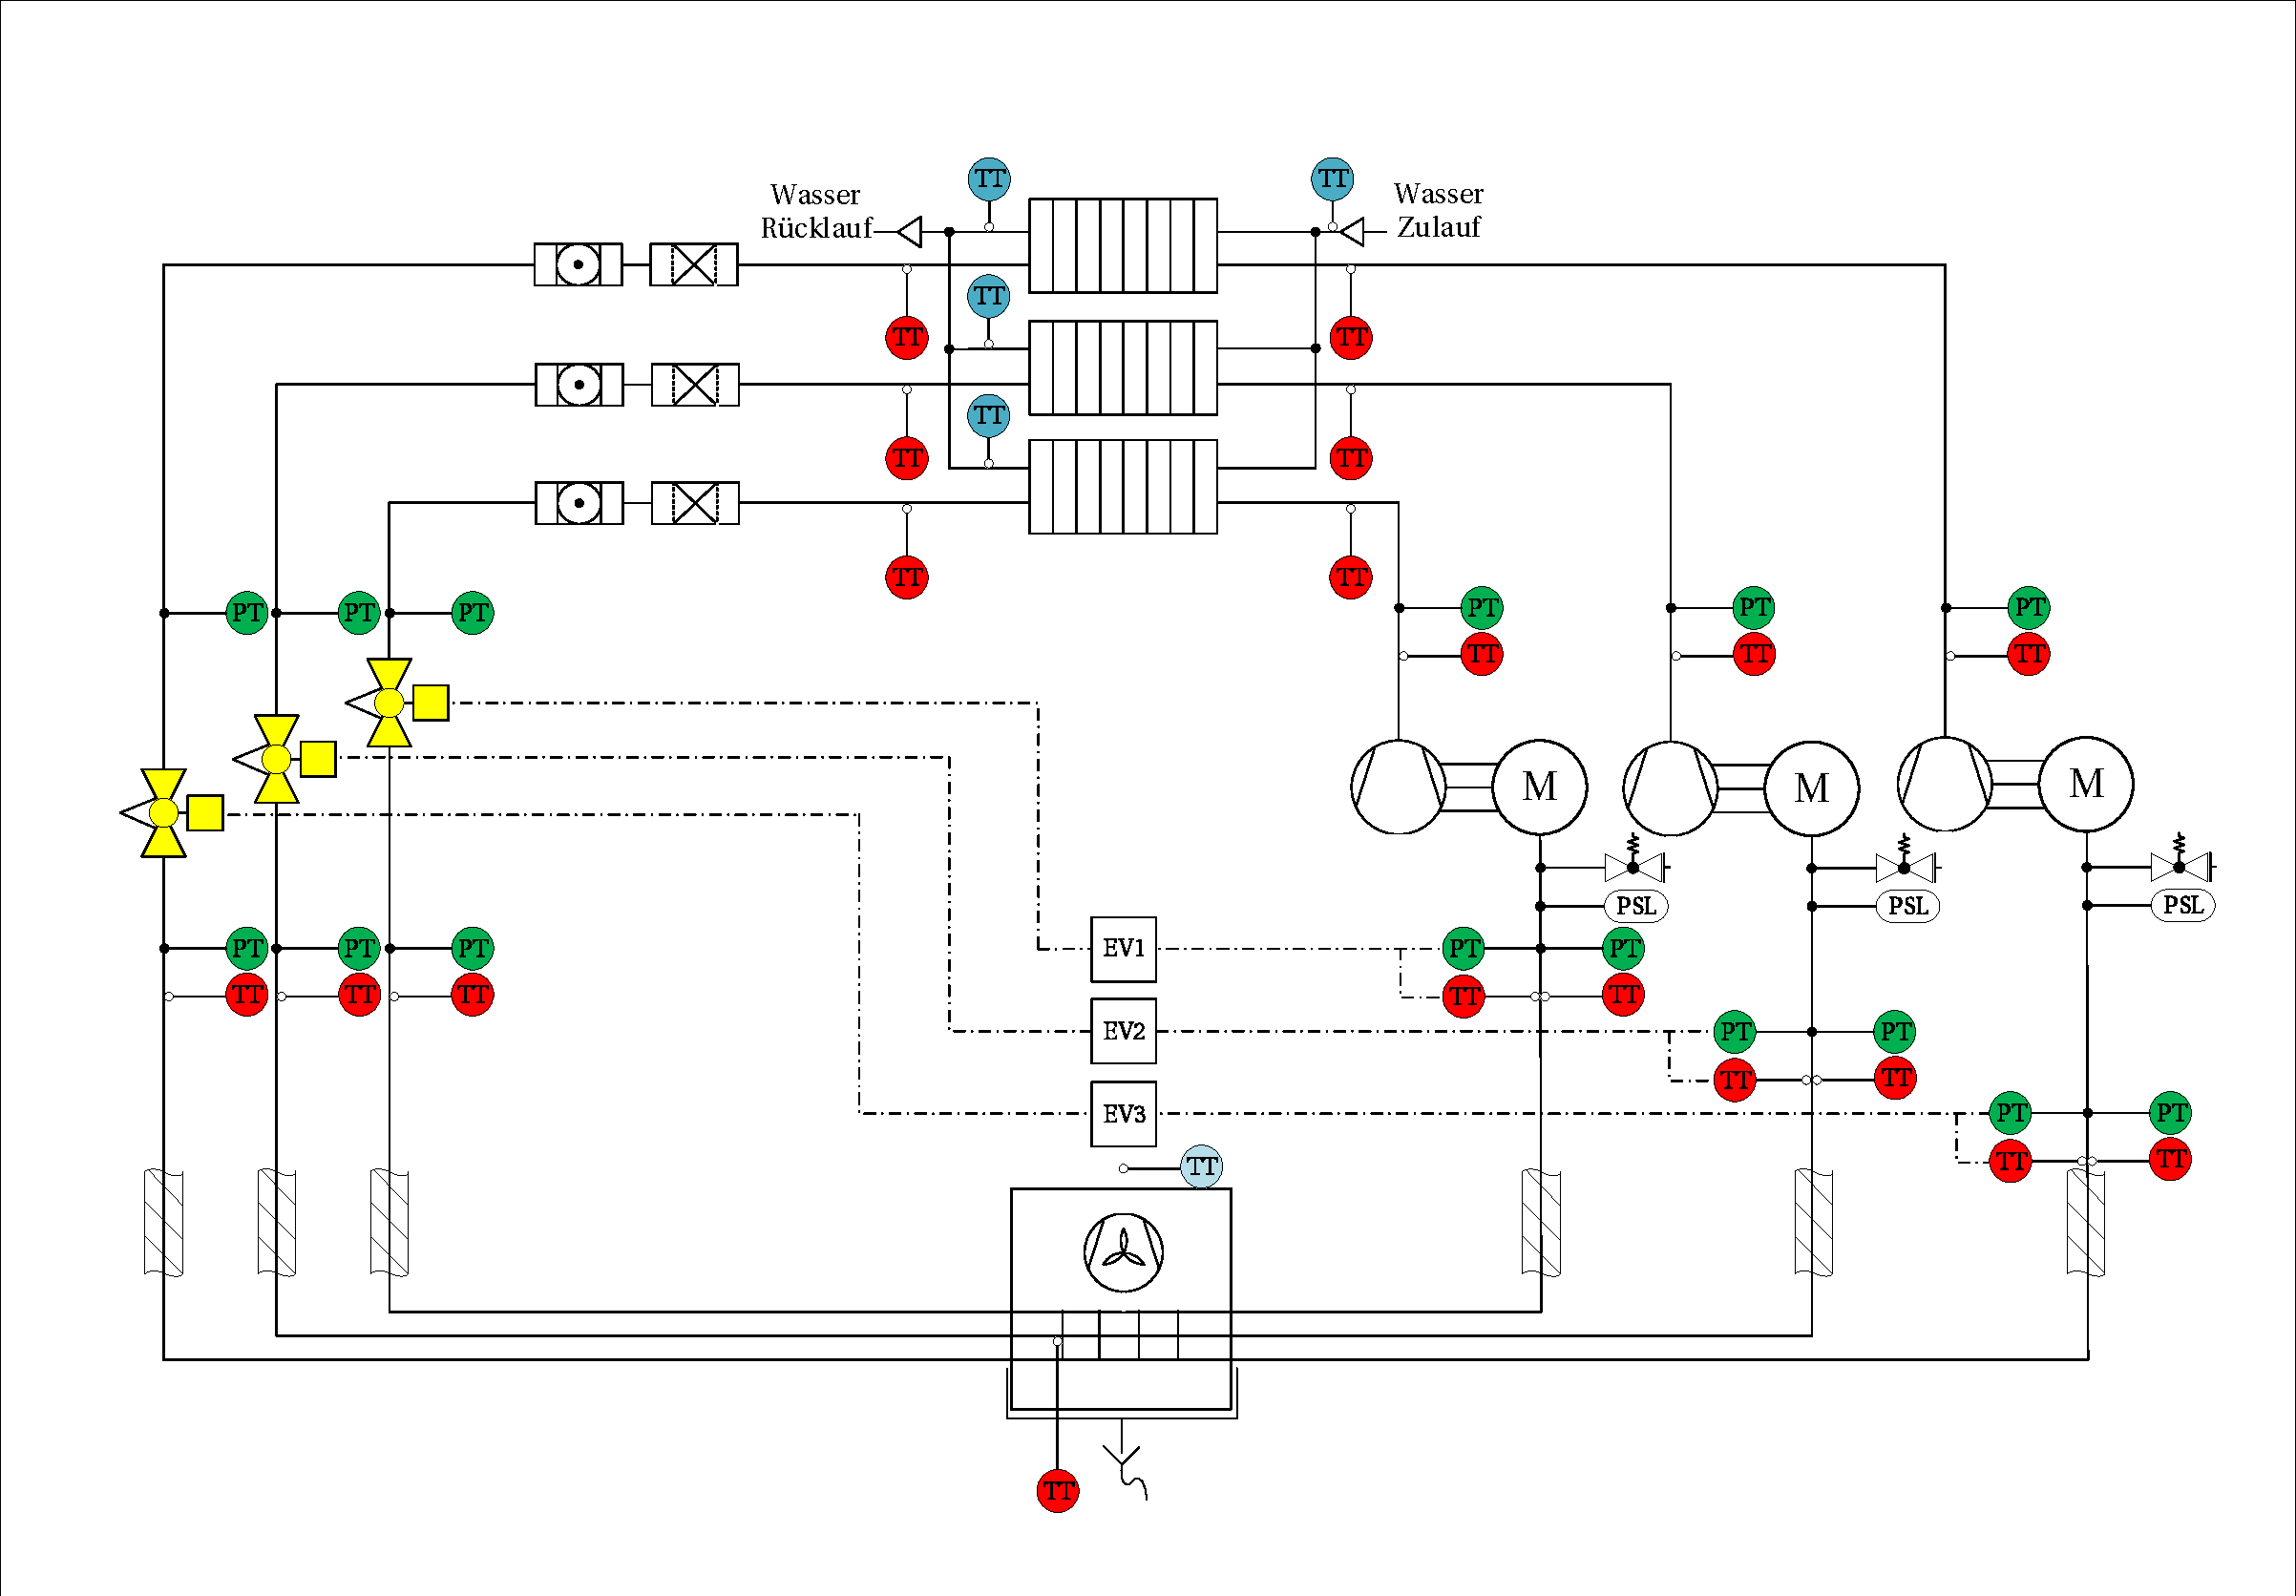
\includegraphics[scale=.5,angle=90]{Pictures/IDC150.pdf}
\caption{IDC150}
\label{fig:IDC150}
\end{figure}


\section{Die Klimakammer}
\label{sec:Die Klimakammer}

Um während den Untersuchungen gleichbleibende Umgebungsbedingungen zu generieren und so reproduzierbare Ergebnisse zu erzielen, steht das Kühlregal in einer Klimakammer.
Wie in Abbildung~\ref{fig:Klimakammer} zu erkennen besteht die Klimakammer eigentlich aus zwei kleineren Kammern mit eigenständigen Zuluftregelungen. Aufgrund der Größe des Regals wurde die Trennwand zwischen den Kammern entfernt. Die Zuluftaufbereitung übernimmt dabei die Klimaanlage der Kammer B. Damit die aufbereitete Luft den Raum über seine gesamte Länge durchströmt wurde die Ansaugöffnung von Kammer B mit einer Decke, die bis zum Ende des Raums reicht, abgedeckt. Vor den Luftauslassgittern besitzen die Kammern Umlenkbleche. Diese sollen eine gleichmäßige Verteilung des Luftmassenstroms über den Austrittquerschnitt erzielen. Die Klimaanlagen sind in der Lage die angesaugte Raumluft zu kühlen, aufzuheizen, sowie zu be- und entfeuchten. Die Regelung findet dabei über einen Computer statt. Mithilfe von LabView, welches eine intuitive Benutzeroberfläche bietet, lässt sich Einfluss auf die Soll-Werte, die Dauer der jeweiligen Untersuchung und die Einstellung der Regelparameter nehmen. 
Jede Kammer besitzt zudem einen Wasseranschluss dessen Vorlauftemperatur regulierbar ist.
Die Verflüssiger des Kühlregals werden mit temperiertem Wasser der Regelung von Kammer A beaufschlagt. 


\begin{figure}[htb]
\centering
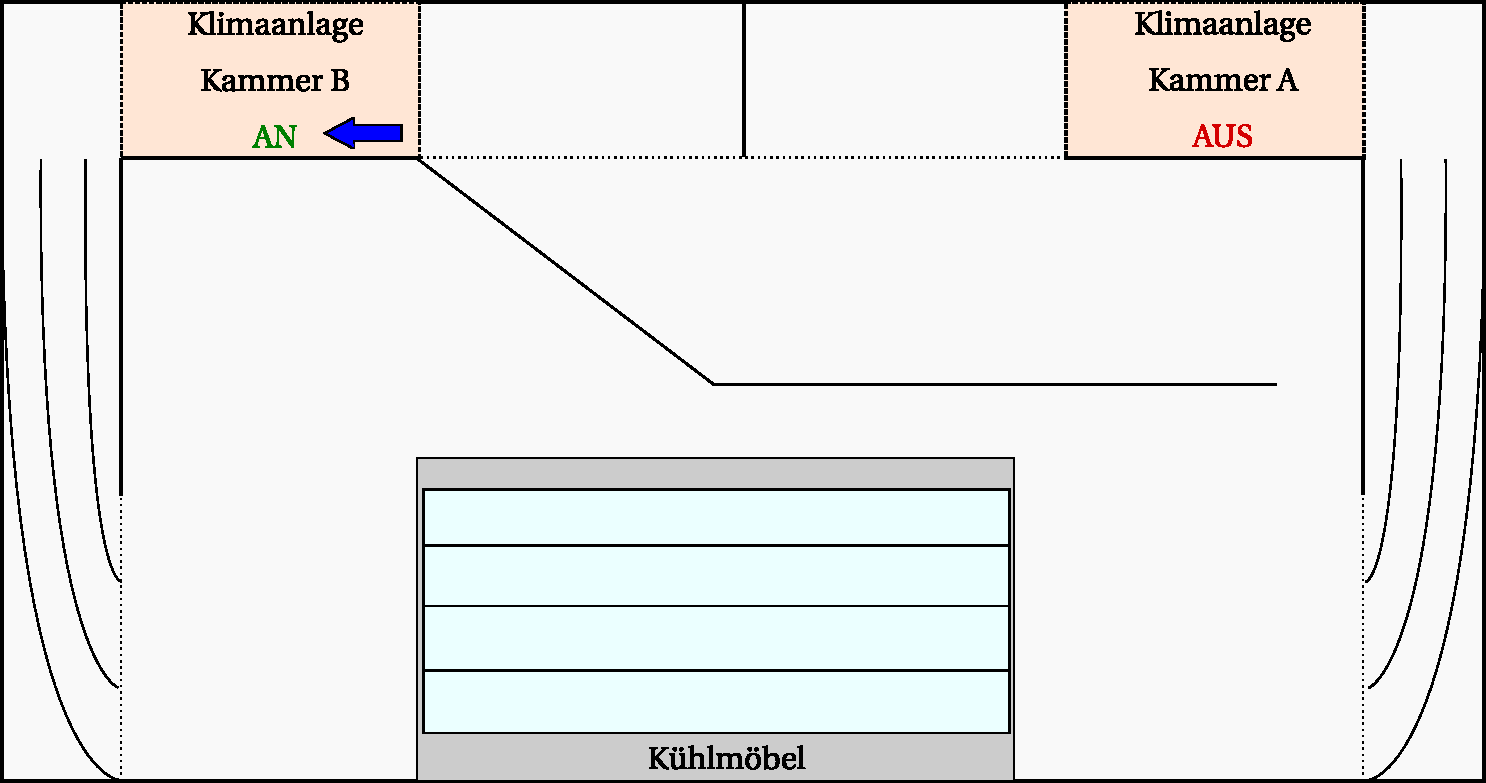
\includegraphics[scale=.5]{Pictures/ClimateChamber.pdf}
\caption{Klimakammer}
\label{fig:Klimakammer}
\end{figure}

\section{Erfassung von Messdaten}
\label{sec:Erfassung von Messdaten}

Um alle physikalischen Größen während des Betriebs möglichst genau zu erfassen und zu speichern werden entsprechende Geräte und Programme eingesetzt. Insgesamt finden drei Systeme Anwendung um sensorbasiert Daten zu erfassen, umzuwandeln und in Tabellenform zu speichern.

\subsection{Messdaten der Klimakammer}
\label{subsec:Messdaten der Klimakammer}

Die in Abschnitt~\ref{sec:Die Klimakammer} vorgestellte Klimakammer wird über LabView gesteuert. Die erfassten Messdaten sind raumluftseitig Ist- und Mittelwerte der Temperaturen sowie die relative Luftfeuchtigkeit. Wasserseitig werden Wassermassenstrom sowie Vor- und Rücklauftemperatur gemessen. 
Die Sensoren, welche die Regelgrößen Temperatur und relative Luftfeuchtigkeit aufnehmen, sind zuluftseitig in der Nähe des Auslassgitters positioniert. Die Regelgröße der Temperatur entspricht dem Mittelwert von drei, über die Höhe des Luftauslassgitters verteilten Temperatursensoren. Wird der Betrieb der Klimakammer über das Programm gestartet so wird eine Exceldatei erstellt in die in einem Intervall von \unit{1}{\second} die erfassten Daten geschrieben werden.


\subsection{Messdaten des Kühlregals}
\label{subsec:Messdaten der Klimakammer}

Mithilfe des Programms NI SignalExpress werden die Messdaten des Kühlregals und der Kältekreisläufe via Modbus erfasst. Um die Temperaturen zu messen werden Thermoelemente  und um die Drücke zu messen Hochgenauigkeitsdruckaufnehmer verwendet. Die erfassten Messwerte sind die Produkttemperaturen sowie Ein- und Austrittstemperatur der Luft am Verdampfer des Kühlregals, die Temperaturen an verschiedenen Positionen der Kältekreisläufe und die Relativdrücke des Kältemittels im System in Heißgasleitung, Flüssigkeitsleitung, Einspritzleitung und Saugleitung. Die Positionen der Sensoren an den Kältekreisläufen sind aus Abbildung~\ref{fig:IDC150} ersichtlich. Zudem wurde noch die Temperatur des Kältemittels nach jedem einzelnen Durchgang durch den Verdampfer erfasst.
In einem Intervall von \unit{5}{\second} werden die erfassten Daten in eine Exceltabelle geschrieben. SignalExpress erstellt in Echtzeit Graphen der Messwerte. Somit lässt sich das Verhalten des Systems jederzeit beobachten.

\subsection{Messdaten des Leistungsanalysators}
\label{subsec:Messdaten des Leistungsanalysators}

Um den Zustand des Systems auch elektroseitig zu erfassen wird ein Yokogawa WT3000 Leistungsanalysator verwendet. Dieser ist in der Lage Spannungen, Ströme mit einer Genauigkeit von \unit{0,02}{\%} zu erfassen und daraus Blind-, Wirk- und Scheinleistungen zu berechnen. Die abgenommenen Komponenten sind die einzelnen Verdichter, die Ventilatoren und die restlichen Verbraucher des Kühlregals, wie Licht und Relays.
Das Gerät speichert die erfassten und berechneten Messwerte in Tabellenform auf einem externen Datenspeicher. Die Intevalllänge beträgt hierbei \unit{5}{\second}.


\section{Testbedingungen nach Norm}
\label{sec:Testbedingungen nach Norm}




 \cite{DINDeutschesInstitutfurNormunge.V..}

% Please add the following required packages to your document preamble:
% \usepackage[table,xcdraw]{xcolor}
% If you use beamer only pass "xcolor=table" option, i.e. \documentclass[xcolor=table]{beamer}
\begin{table}[]
\centering
\caption{Klimaklassen~\cite{DINDeutschesInstitutfurNormunge.V..}}
\label{tab:Klimaklassen}
\begin{tabular}{|c|c|c|c|c|}
\hline
\textbf{\begin{tabular}[c]{@{}c@{}}Klimaklasse des \\ Prüfraums\end{tabular}} & \textbf{\begin{tabular}[c]{@{}c@{}}Trockenkugel-\\ temperatur\end{tabular}} & \textbf{\begin{tabular}[c]{@{}c@{}}Relative \\ Luftfeuchte\end{tabular}} & \textbf{Taupunkt} & \textbf{\begin{tabular}[c]{@{}c@{}}Wasserdampf-\\ gehalt \\ in trockener Luft\end{tabular}} \\
                                                                              &                                                                             & \%                                                                       & °C                & g/kg                                                                                        \\ \hline
0                                                                             & 20                                                                          & 50                                                                       & 9,3               & 7,3                                                                                         \\ \hline
1                                                                             & 16                                                                          & 80                                                                       & 12,6              & 9,1                                                                                         \\ \hline
8                                                                             & 23,9                                                                        & 55                                                                       & 14,3              & 10,2                                                                                        \\ \hline
2                                                                             & 22                                                                          & 65                                                                       & 15,2              & 10,8                                                                                        \\ \hline
\rowcolor[HTML]{FFFe65}
3                                                                             & 25                                                                          & 60                                                                       & 16,7              & 12                                                                                          
\\ \hline
4                                                                             & 30                                                                          & 55                                                                       & 20                & 14,8                                                                                        \\ \hline
5                                                                             & 27                                                                          & 70                                                                       & 21,1              & 15,8                                                                                        \\ \hline
6                                                                             & 40                                                                          & 40                                                                       & 23,9              & 18,8                                                                                        \\ \hline
7                                                                             & 35                                                                          & 75                                                                       & 30                & 27,3                                                                                        \\ \hline
\end{tabular}
\end{table}


% Please add the following required packages to your document preamble:
% \usepackage[table,xcdraw]{xcolor}
% If you use beamer only pass "xcolor=table" option, i.e. \documentclass[xcolor=table]{beamer}
\begin{table}[]
\centering
\caption{Temperaturklassen der M-Pakete~\cite{DINDeutschesInstitutfurNormunge.V..}}
\label{tab:Temperaturklassen}
\begin{tabular}{|c|c|c|}
\hline
\textbf{Klasse} & \textbf{\begin{tabular}[c]{@{}c@{}}Höchste Temperatur,\\ des wärmsten\\ M-Pakets gleich oder\\ niedriger als\end{tabular}} & \textbf{\begin{tabular}[c]{@{}c@{}}Niedrigste Temperatur,\\ des kältesten\\ M-Pakets gleich oder\\ höher als\end{tabular}} \\ \cline{2-3} 
                & \multicolumn{2}{c|}{°C}                                                                                                                                                                                                                                 \\ \hline
L1              & -15                                                                                                                        & -                                                                                                                          \\ \hline
L2              & -12                                                                                                                        & -                                                                                                                          \\ \hline
L3              & -12                                                                                                                        & -                                                                                                                          \\ \hline
\rowcolor[HTML]{FFFE65} 
M1              & +5                                                                                                                         & -1                                                                                                                         \\ \hline
M2              & +7                                                                                                                         & -1                                                                                                                         \\ \hline
H1              & +10                                                                                                                        & +1                                                                                                                         \\ \hline
H2              & +10                                                                                                                        & -1                                                                                                                         \\ \hline
S               & \multicolumn{2}{c|}{Sonderklasse}                                                                                                                                                                                                                       \\ \hline
\end{tabular}
\end{table}



\begin{figure}[htb]
\centering
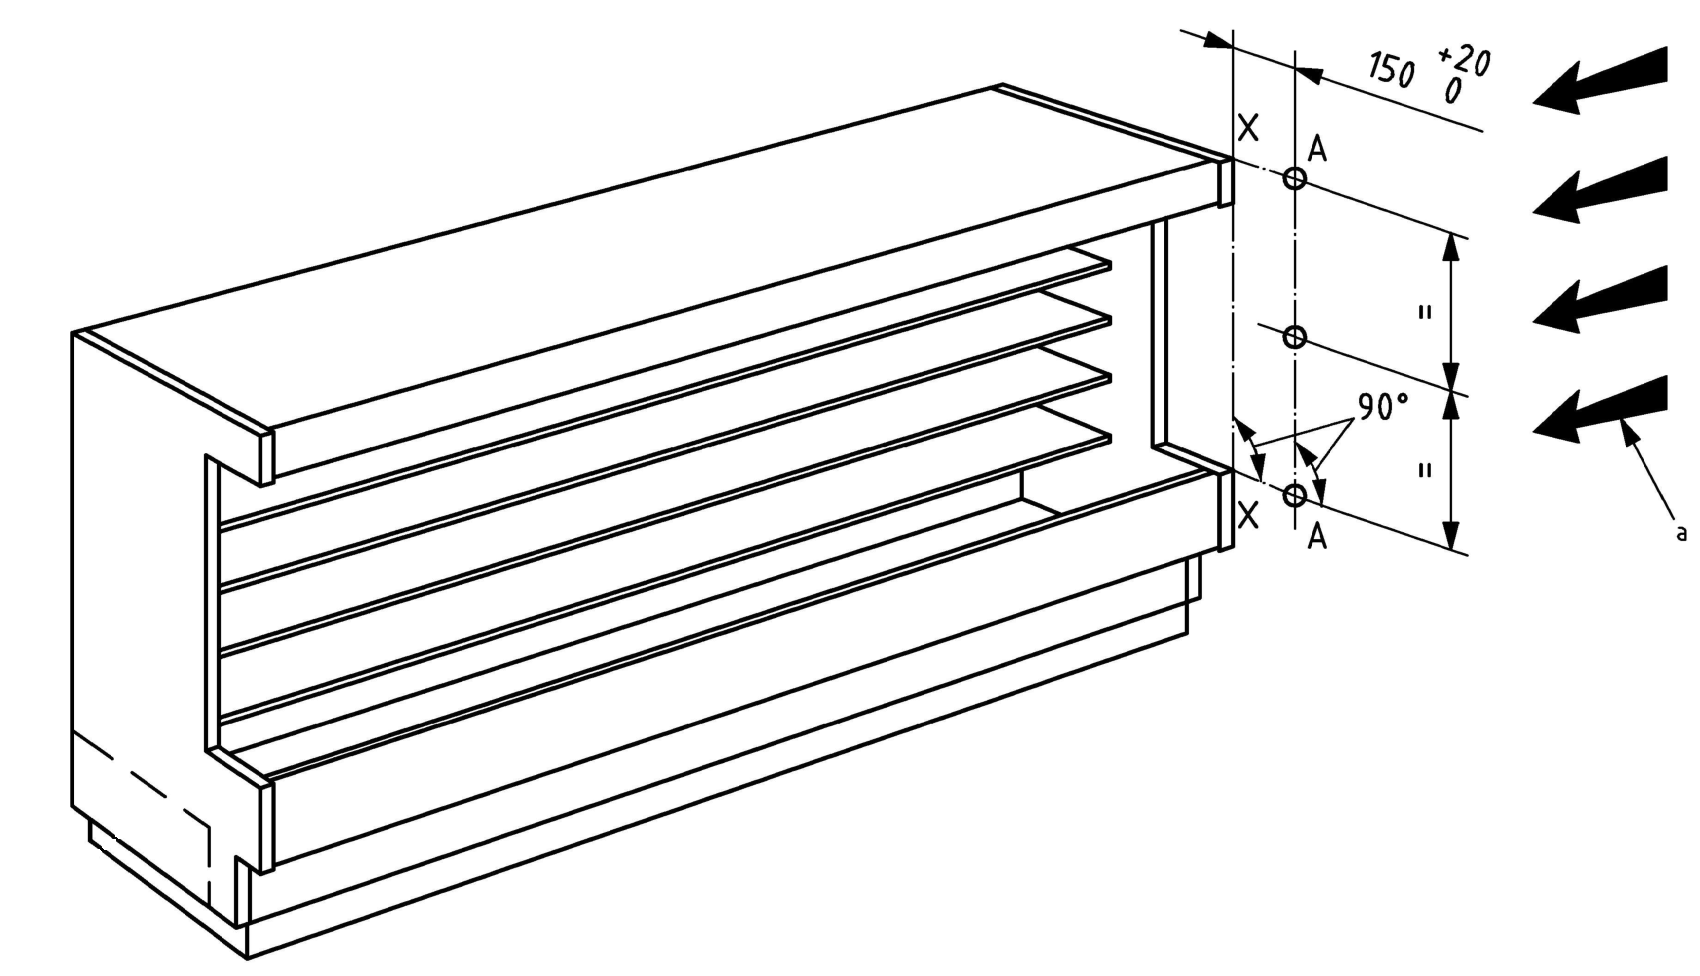
\includegraphics[scale=.5]{Pictures/idc_meas.pdf}
\caption{Messpunkte~\cite{DINDeutschesInstitutfurNormunge.V..}}
\label{fig:Messpunkte}
\end{figure}







\chapter{Prüfstand}
\label{cha:Prüfstand}





%\begin{figure}[h]
%   \centering
%   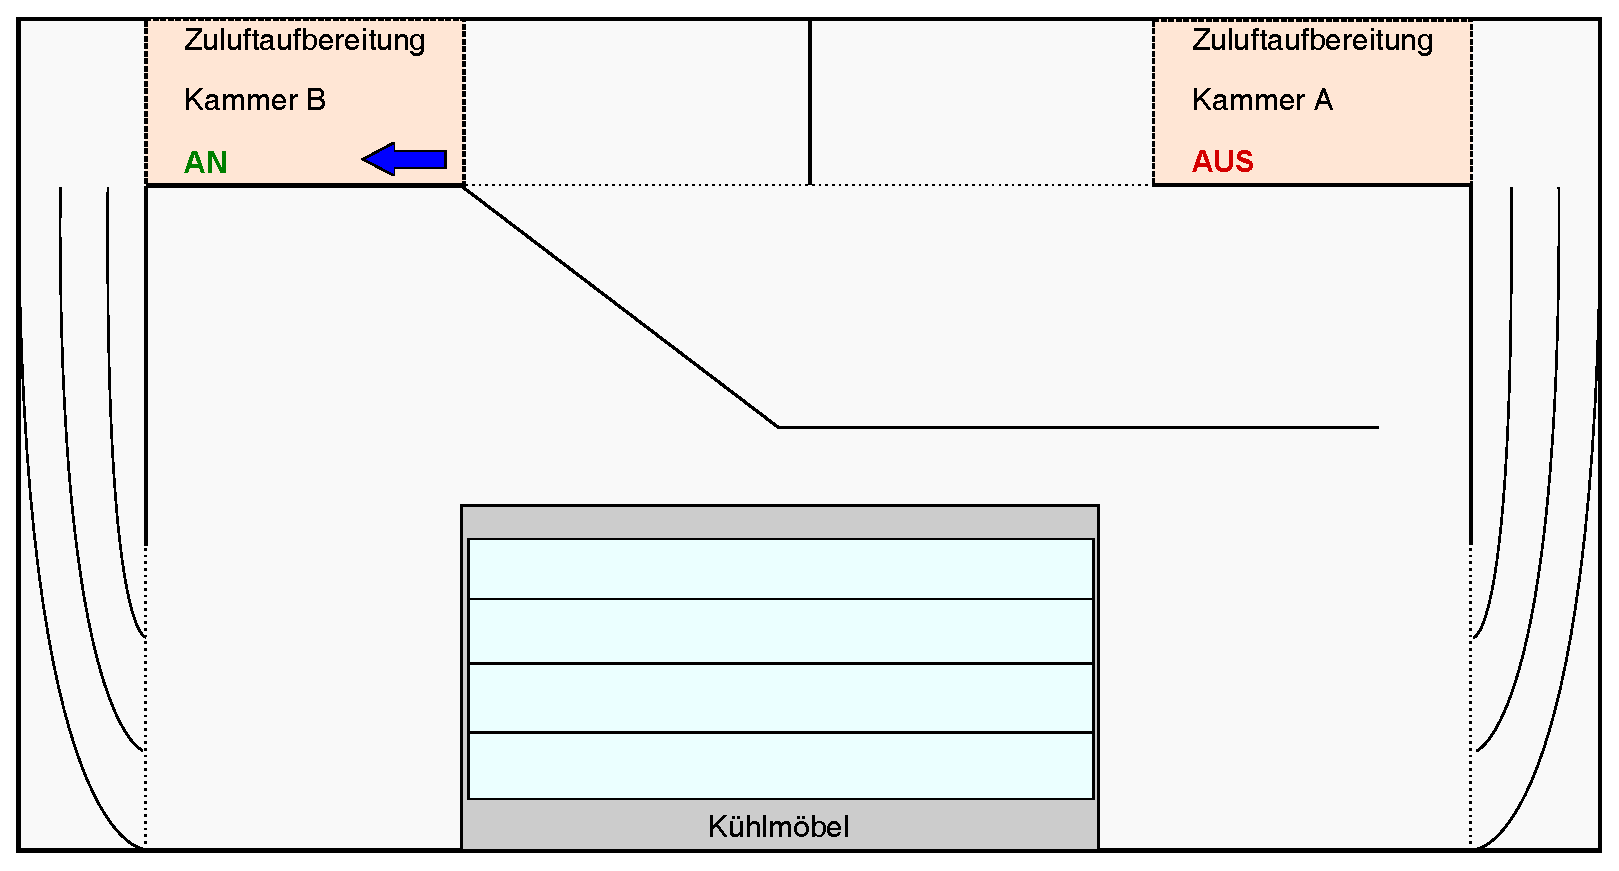
\includegraphics{Pictures/ClimateChamber.eps}
%\end{figure}

Grafiken:
Klimakammer Inkscape
Quellen:
DIN EN ISO 23953
%\chapter{Versuchsdurchführung}
\label{cha:Versuchsdurchführung}

Aus den Versuchsdaten wissen wir, dass nur die letzte Rohrstrecke überhitzt ist.

\chapter{Analyse der Messergebnisse}
\label{cha:Analyse der Messergebnisse}

\chapter{Zusammenfassung}
\label{cha:Zusammenfassung}
Verweis auf Sektion: (siehe \ref{subsec:Abschnitt1})
%\chapter{Analyse der Messergebnisse}
\label{cha:Analyse der Messergebnisse}

\chapter{Zusammenfassung}
\label{cha:Zusammenfassung}
Verweis auf Sektion: (siehe \ref{subsec:Abschnitt1})


%-----------------------------------------------------------------------------
% Literaturverzeichnis
%-----------------------------------------------------------------------------

\clearpage
\refstepcounter{Hilfszaehler}
\addcontentsline{toc}{chapter}{\bibname}
\protect\bibliographystyle{unsrt} %unsrt%natdin Dieser Stil ist eine Empfehlung, aber nicht verpflichtend.
\bibliography{Literaturverzeichnis}

%-----------------------------------------------------------------------------
% Anhang
%-----------------------------------------------------------------------------
\pagestyle{empty}
\clearpage
\vfill{}\vspace{-1\parskip}
\begin{center}\textsf{\textbf{\huge Anhang}}\end{center}{\huge \par}
\vfill{}
\appendix
\newpage
\pagestyle{scrheadings}
\chapter{Grafische Auswertung der Untersuchungen}

\section{Untersuchung 35}

\begin{figure}[h!]
\centering
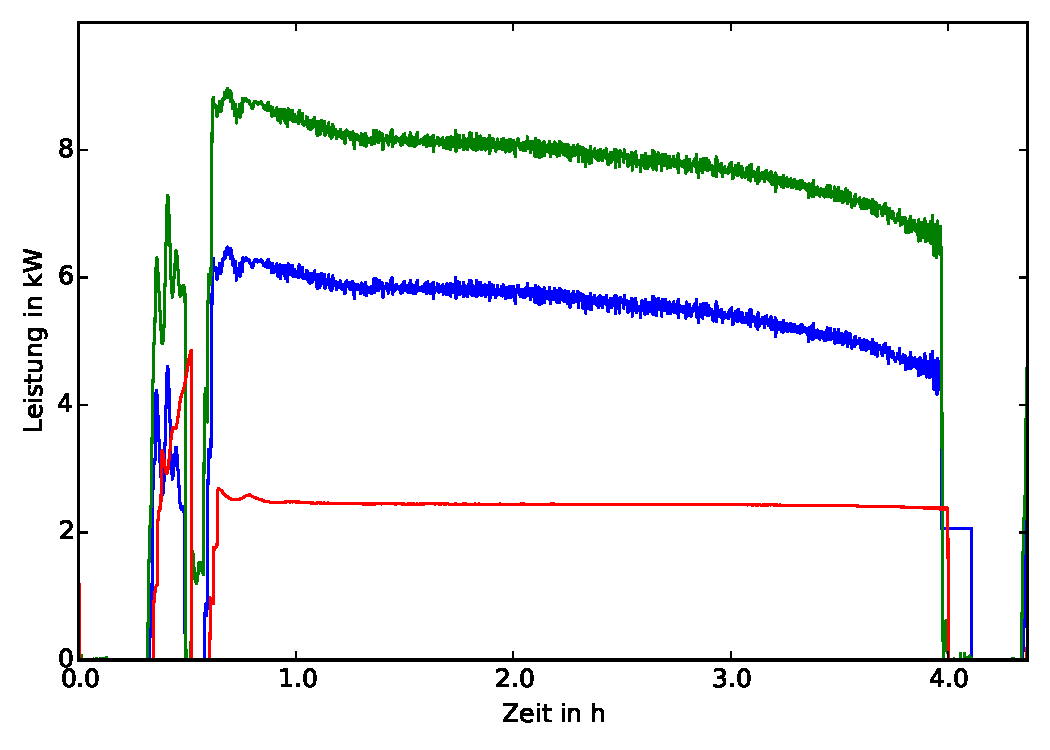
\includegraphics[scale=0.8]{Pictures/35/Qdots_lastCycle.pdf}
\caption{Leistungen beim Betrieb mit 3MAF.}
\label{fig:Leistungen35}
\end{figure}

\begin{figure}[h!]
\centering
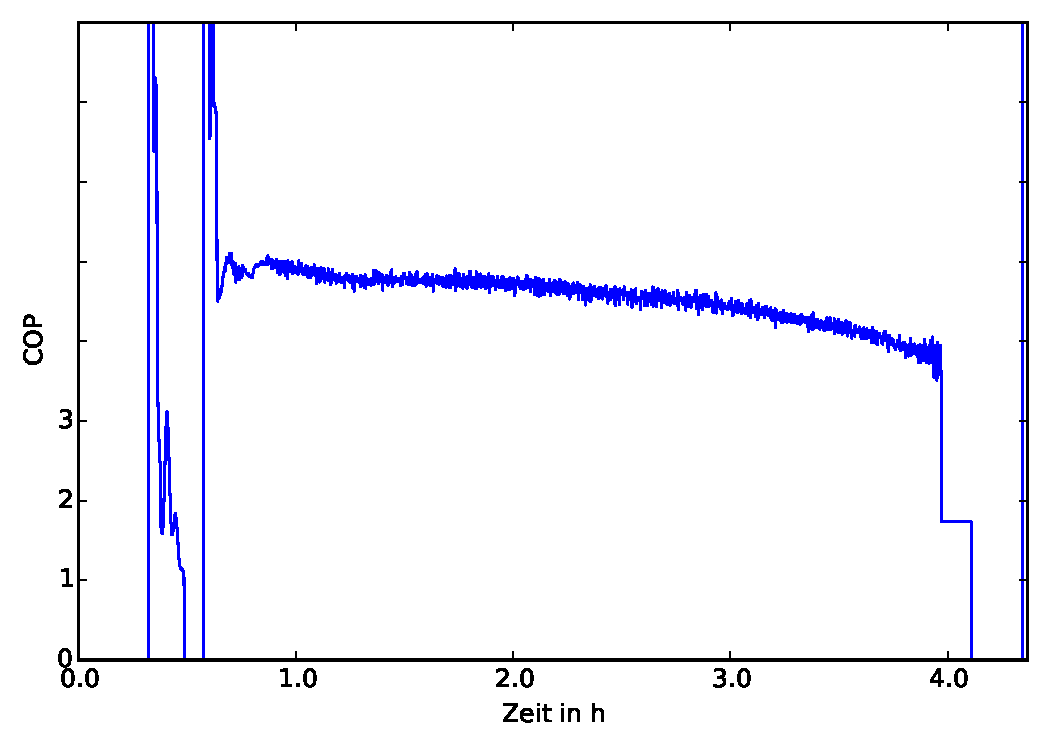
\includegraphics[scale=0.8]{Pictures/35/COP_lastCycle.pdf}
\caption{COP beim Betrieb mit 3MAF.}
\label{fig:COP35}
\end{figure}

\begin{figure}[h!]
\centering
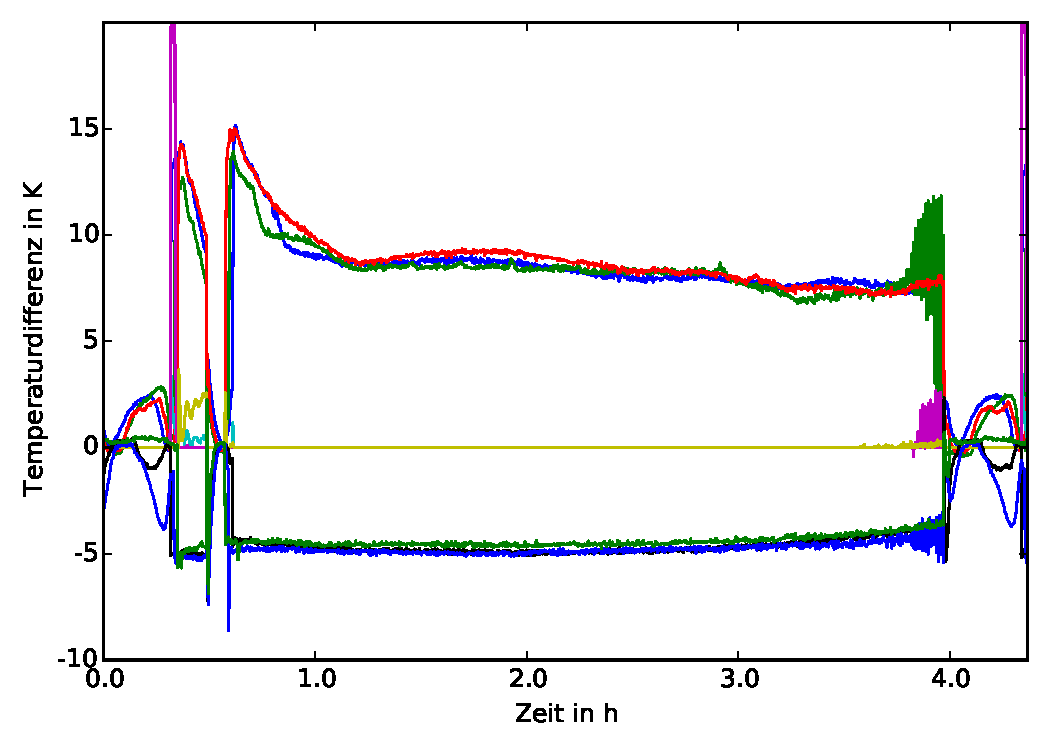
\includegraphics[scale=0.8]{Pictures/35/deltaTs_lastCycle.pdf}
\caption{Überhitzung und Unterkühlung (K1) beim Betrieb mit 3MAF.}
\label{fig:deltaT35}
\end{figure}

\begin{figure}[h!]
\centering
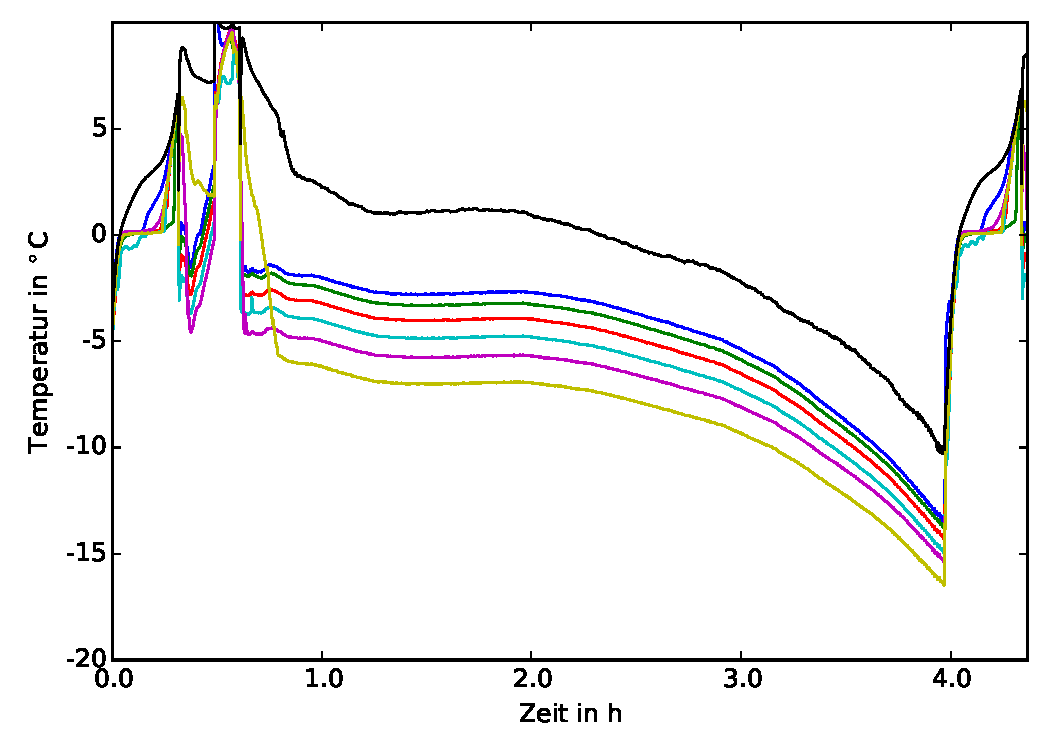
\includegraphics[scale=0.8]{Pictures/35/T_evap_C1_lastCycle.pdf}
\caption{Temperaturen im Verdampfer (K1) beim Betrieb mit 3MAF.}
\label{fig:deltaT35}
\end{figure}

\begin{figure}[h!]
\centering
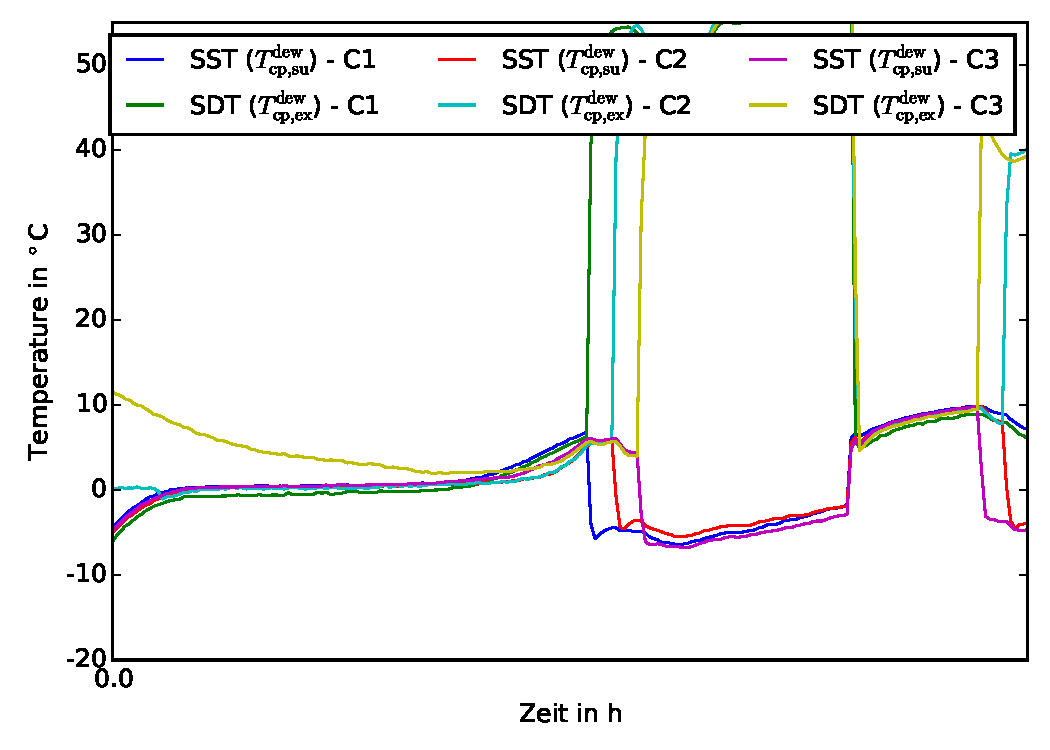
\includegraphics[scale=0.8]{Pictures/35/Tsats_lastCycle.pdf}
\caption{Sättigungstemperaturen (K1) beim Betrieb mit 3MAF.}
\label{fig:Tsats35}
\end{figure}

\begin{figure}[h!]
\centering
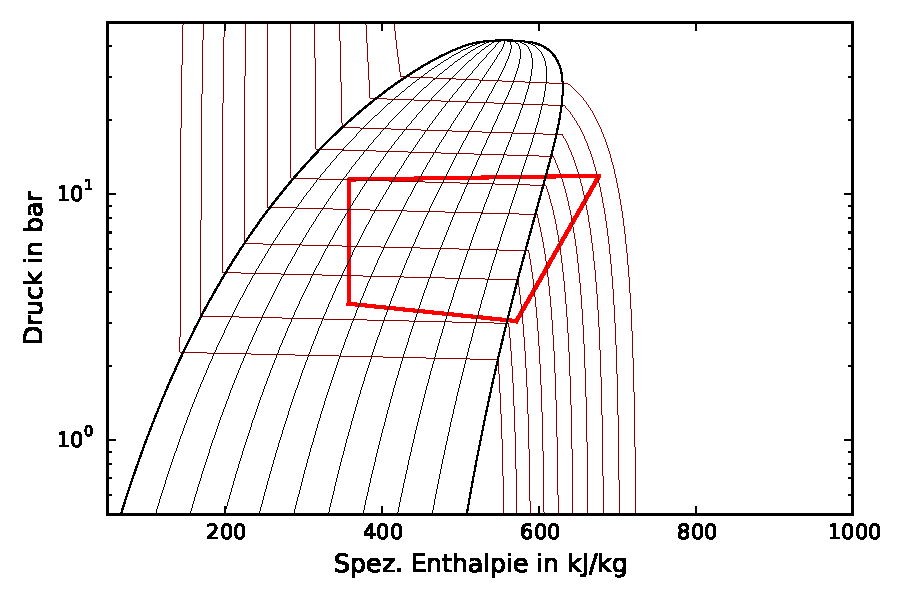
\includegraphics[scale=0.8]{Pictures/35/log_ph_lastCycle10perc_C1.pdf}
\caption{logp-h-Diagramm (K1) beim Betrieb mit 3MAF \unit{10}{\%} vor Ende des Zyklus.}
\label{fig:logph35}
\end{figure}

\begin{figure}[h!]
\centering
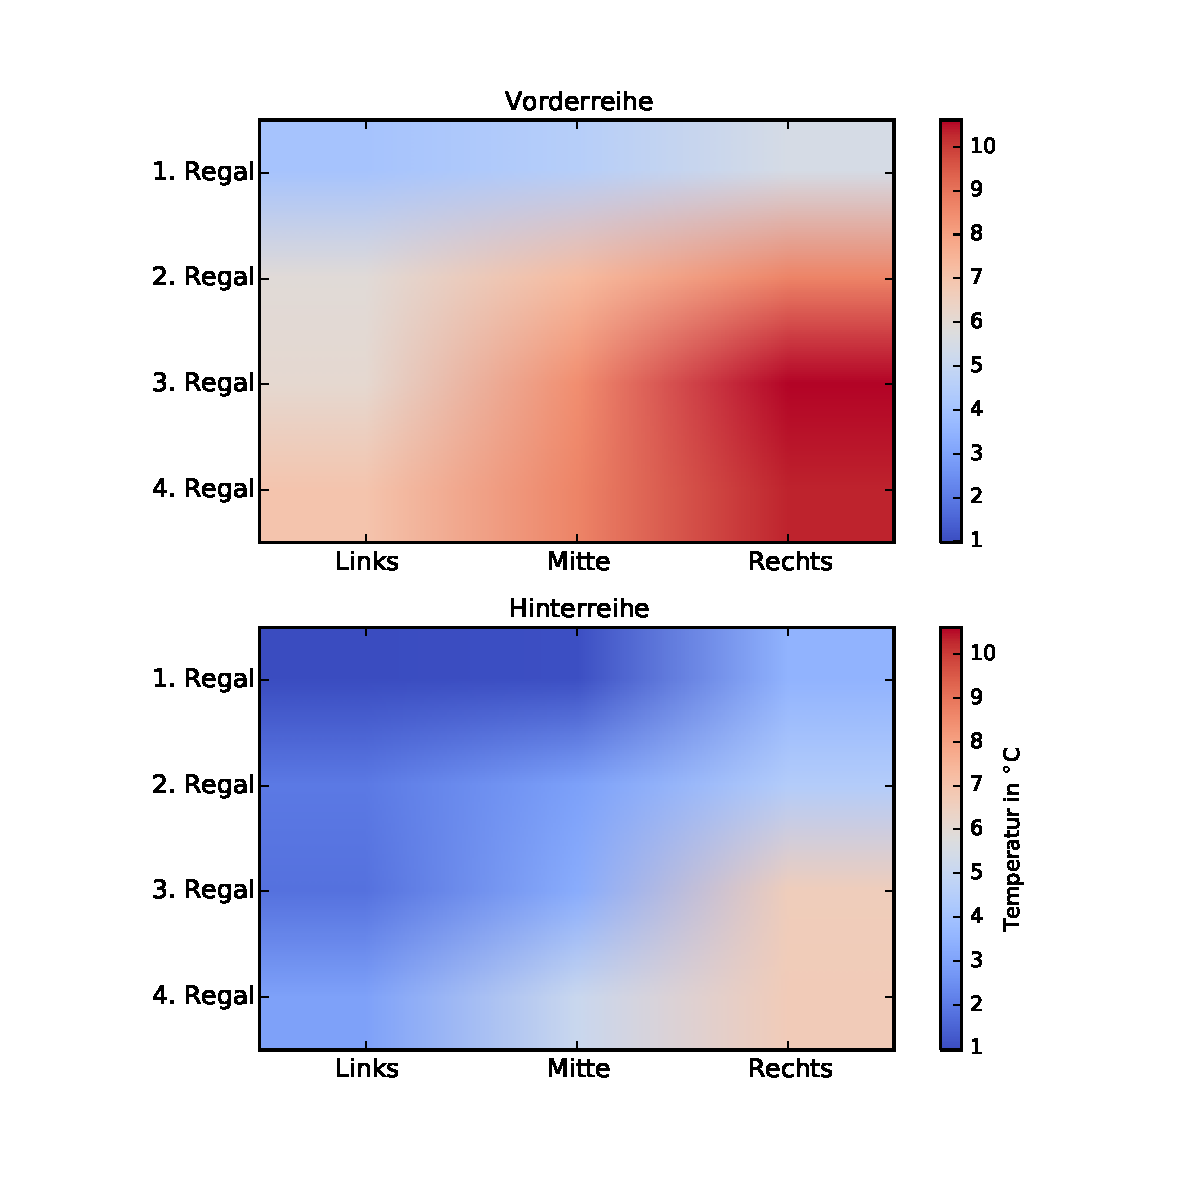
\includegraphics[scale=0.8]{Pictures/35/load_colormap_lastCycle10perc.pdf}
\caption{Produkttemperaturen in der vorderen und hinteren Regalreihe beim Betrieb mit 3MAF.}
\label{fig:prodtempmap35}
\end{figure}

\begin{figure}[h!]
\centering
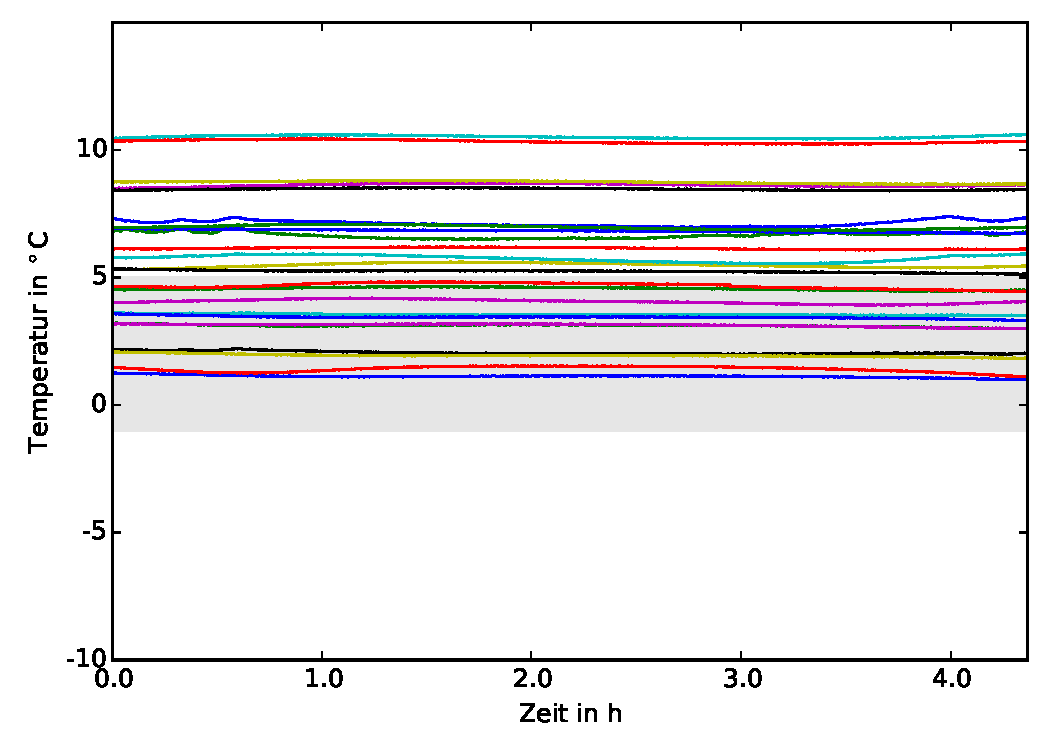
\includegraphics[scale=0.8]{Pictures/35/ProductTemperature.pdf}
\caption{Produkttemperaturen beim Betrieb mit 3MAF.}
\label{fig:prodtemp35}
\end{figure}



\section{Untersuchung 50}

\begin{figure}[h!]
\centering
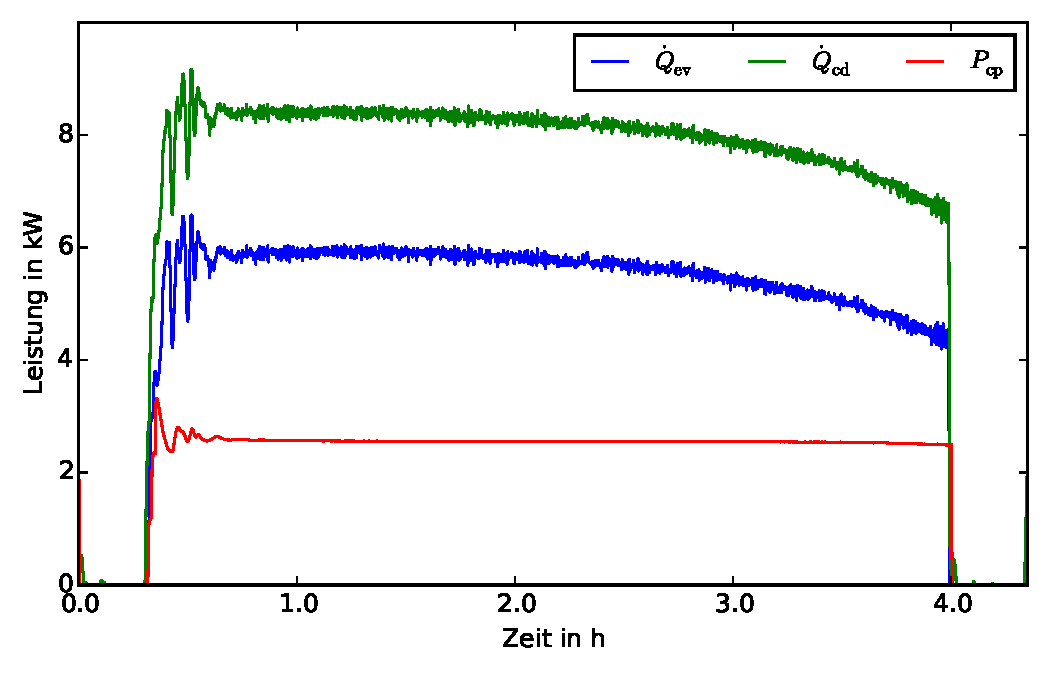
\includegraphics[scale=0.8]{Pictures/50/Qdots_lastCycle.pdf}
\caption{Leistungen beim Betrieb mit einem 4h Abtauintervall.}
\label{fig:Leistungen50}
\end{figure}

\begin{figure}[h!]
\centering
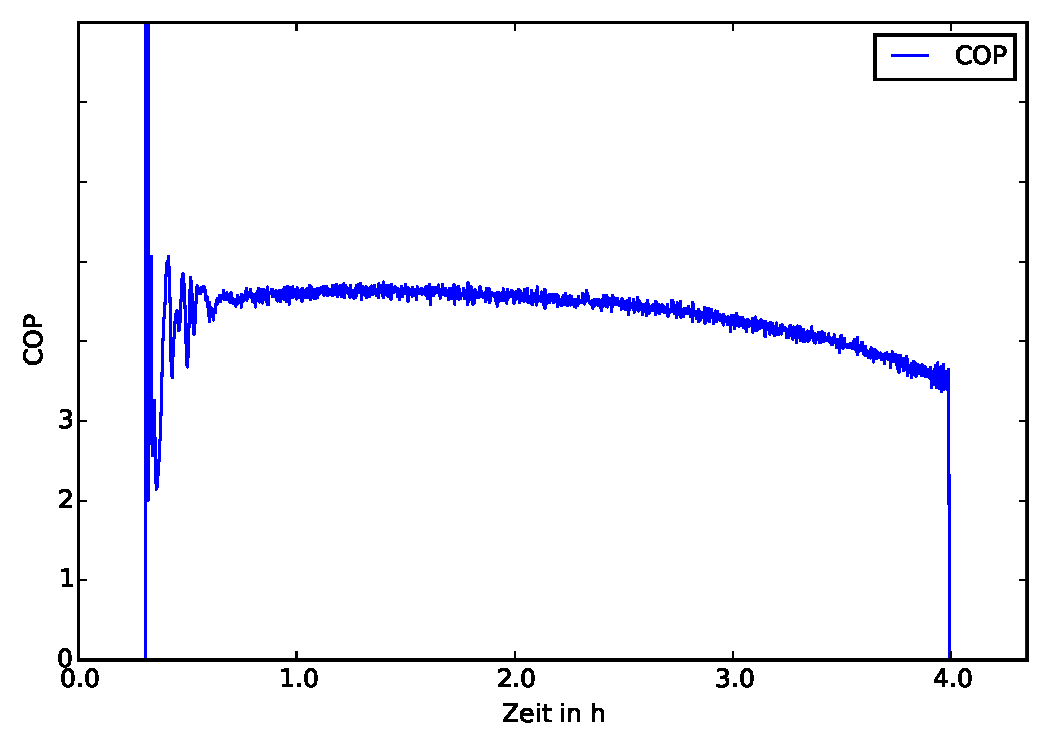
\includegraphics[scale=0.8]{Pictures/50/COP_lastCycle.pdf}
\caption{COP beim Betrieb mit einem 4h Abtauintervall.}
\label{fig:COP50}
\end{figure}

\begin{figure}[h!]
\centering
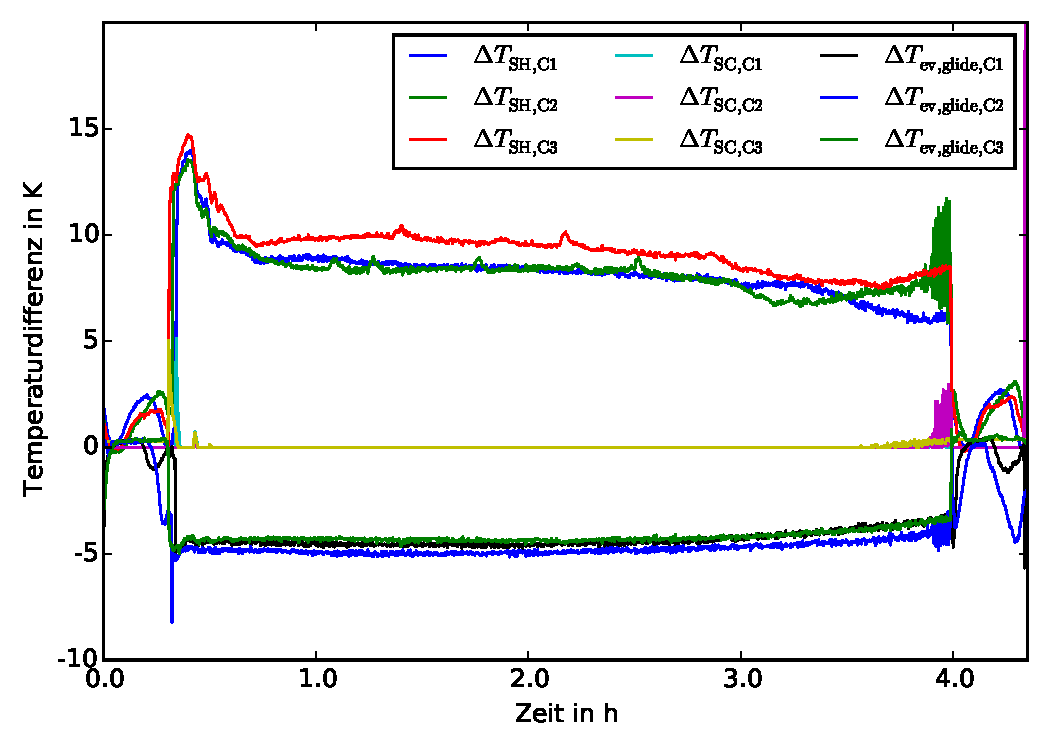
\includegraphics[scale=0.8]{Pictures/50/deltaTs_lastCycle.pdf}
\caption{Überhitzung und Unterkühlung (K1) beim Betrieb mit einem 4h Abtauintervall.}
\label{fig:deltaT50}
\end{figure}

\begin{figure}[h!]
\centering
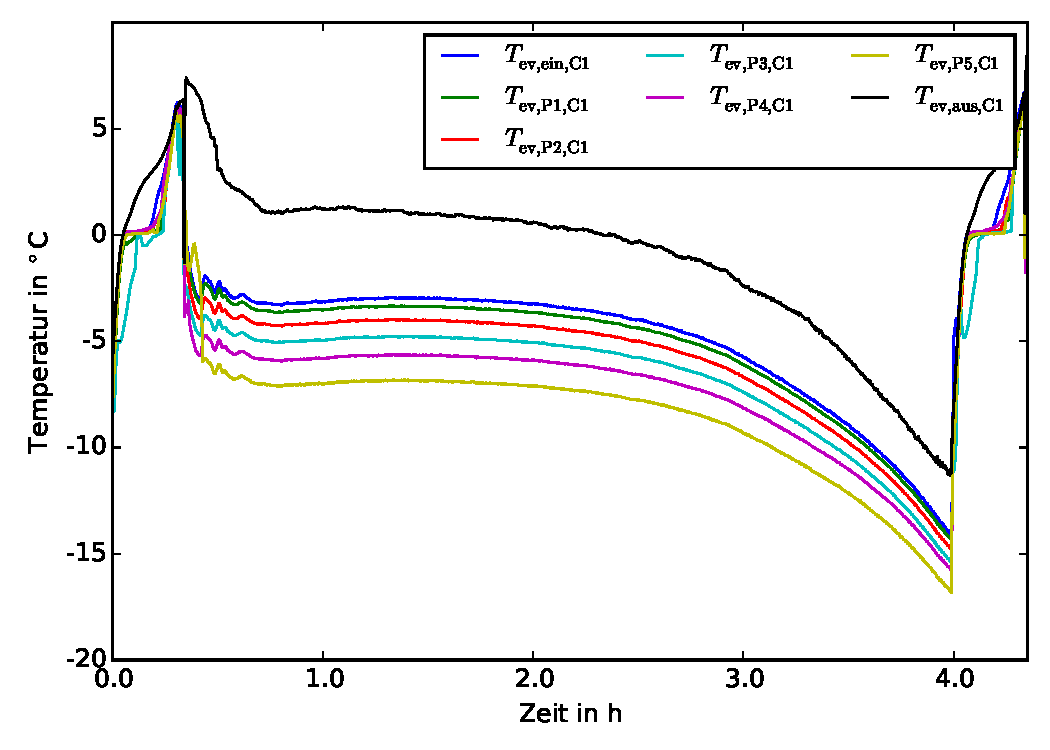
\includegraphics[scale=0.8]{Pictures/50/T_evap_C1_lastCycle.pdf}
\caption{Temperaturen im Verdampfer (K1) beim Betrieb mit einem 4h Abtauintervall.}
\label{fig:deltaT50}
\end{figure}

\begin{figure}[h!]
\centering
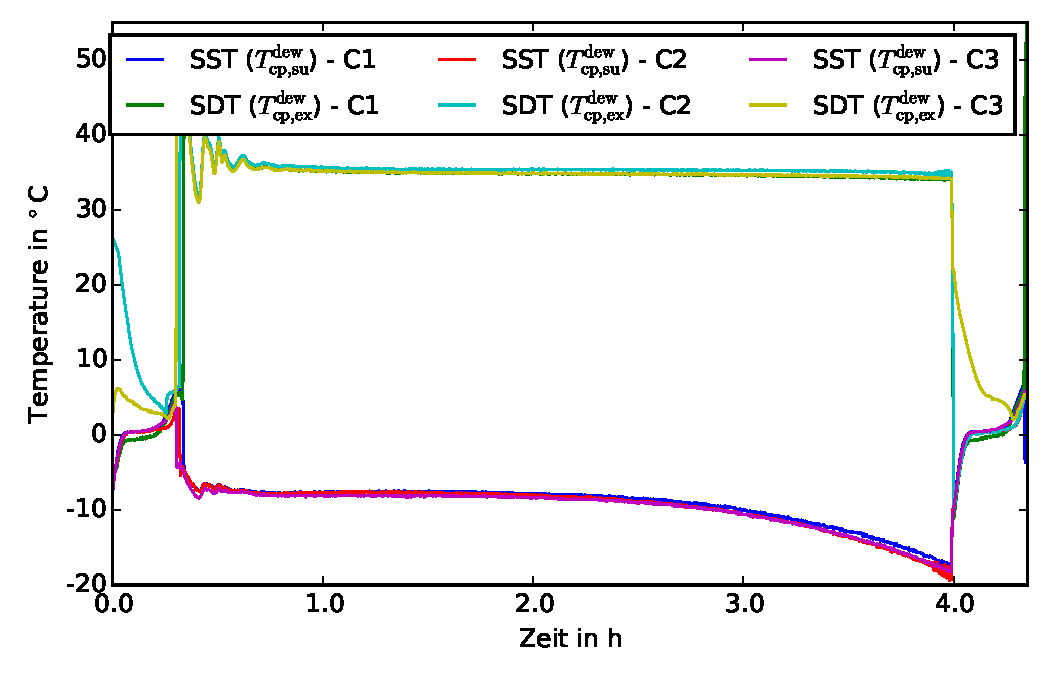
\includegraphics[scale=0.8]{Pictures/50/Tsats_lastCycle.pdf}
\caption{Sättigungstemperaturen (K1) beim Betrieb mit einem 4h Abtauintervall.}
\label{fig:Tsats50}
\end{figure}

\begin{figure}[h!]
\centering
\includegraphics[scale=0.8]{Pictures/50/log_ph_lastCycle10perc_C1.pdf}
\caption{logp-h-Diagramm (K1) beim Betrieb mit einem 4h Abtauintervall \unit{10}{\%} vor Ende des Zyklus.}
\label{fig:logph50}
\end{figure}

\begin{figure}[h!]
\centering
\includegraphics[scale=0.8]{Pictures/50/load_colormap_lastCycle10perc.pdf}
\caption{Produkttemperaturen in der vorderen und hinteren Regalreihe beim Betrieb mit einem 4h Abtauintervall.}
\label{fig:prodtempmap50}
\end{figure}

\begin{figure}[h!]
\centering
\includegraphics[scale=0.8]{Pictures/50/ProductTemperature.pdf}
\caption{Produkttemperaturen beim Betrieb mit einem 4h Abtauintervall.}
\label{fig:prodtemp50}
\end{figure}


\section{Betrieb mit 3h Abtauintervall}

\section{Betrieb mit ZB09KAU-TFD (Kupferwicklung)}

\section{Betrieb mit ZB09KAU-TFD (Aluminiumwicklung}

\section{Betrieb mit AHT Verdampfer}

\section{Betrieb mit LIDL Verdampfer V1 bei 0\% r.F.}

\section{Betrieb mit LIDL Verdampfer V1 bei 60\% r.F.}

\section{Betrieb mit LIDL Verdampfer V2 bei 0\% r.F.}

\section{Betrieb mit LIDL Verdampfer V2 bei 60\% r.F.}


%-----------------------------------------------------------------------------
% Eigenstaendigkeitserklaerung
%-----------------------------------------------------------------------------
\pagestyle{empty}
\cleardoublepage
\Large
\textbf{Eigenständigkeitserklärung}

\normalsize
Hiermit versichere ich, dass ich die vorliegende Arbeit selbstständig und ohne Benutzung anderer als der angegebenen Hilfsmittel angefertigt habe. Alle Stellen, die wörtlich oder sinngemäß übernommen sind, sind als solche kenntlich gemacht. Die Arbeit ist in gleicher oder ähnlicher Form noch nicht als Prüfungsarbeit eingereicht worden. Ich erkläre mich damit einverstanden, dass die vorliegende Arbeit in der Lehrstuhlbibliothek und Datenbank aufbewahrt und für den internen Gebrauch kopiert werden darf. \newline \newline


Aachen, den \today \newline \newline

%TODO Name ergänzen
Tim Klebig



\end{document}